% CausalCGM-MT -- ML4H 2026 Findings Track, camera-ready version.
%
% Build:  pdflatex main && bibtex main && pdflatex main && pdflatex main
%
% Every inline number resolves through a macro in numbers.tex, and every table
% is \input from runs/paper_results/. Both are regenerated by
%     python scripts/rebuild_paper_tables.py
% directly from the experiment JSON, so the prose cannot drift from the results.
%
% The Findings Track sets no page limit for the camera-ready. Secondary
% validations live in sections/ and are \input after the back matter, on a new
% page after the bibliography.
\documentclass[pmlr,twocolumn,10pt]{jmlr}

% ML4H 2026 track. The paper was accepted to the Findings Track.
\mlhtrack{findings}

\newif\iffinal
\finaltrue  % camera-ready

\iffinal
    % The class would otherwise print the `pmlr' option's "Proceedings of
    % Machine Learning Research" in the upper left. The acceptance email
    % requires "ML4H 2026 - Findings Track" there.
    \jmlrproceedings{}{ML4H 2026 - \mlhtrackname}
    \jmlrworkshop{Machine Learning for Health (ML4H) 2026}
\else
    \jmlrproceedings{}{Submitted to ML4H 2026: \mlhtrackname}
    \jmlrworkshop{Machine Learning for Health (ML4H) 2026}
\fi

\urlstyle{same}

% amsmath, amssymb, natbib, graphicx, url, xcolor, hyperref and algorithm2e are
% loaded by jmlr.cls -- do not re-load them here. Only booktabs is additional;
% the generated tables in runs/paper_results/ use \toprule/\midrule/\bottomrule
% and \resizebox (graphicx).
\usepackage{booktabs}
% Landscape floats for the two sixteen-column benchmark tables (Appendix B).
\usepackage{rotating}
\graphicspath{{figures/}}
% Generated by scripts/rebuild_paper_tables.py -- do not edit.
% Every inline number in main.tex resolves through these macros.

\newcommand{\NumSubjects}{12}
\newcommand{\NumFitWindows}{96{,}692}
\newcommand{\NumValWindows}{11{,}699}
\newcommand{\NumTestWindows}{28{,}335}
\newcommand{\NumEmbargoed}{802}
\newcommand{\NumCalibWindows}{12{,}131}
\newcommand{\NumAlpha}{0.10}
\newcommand{\NumLGBMRMSEGapHThirty}{0.05}
\newcommand{\NumLGBMRMSEGapPctHThirty}{0.3}
\newcommand{\NumFusionRMSELeadHThirty}{0.05}
\newcommand{\NumFusionRMSELeadPctHThirty}{0.3}
\newcommand{\NumFusionPRAUCGapHThirty}{+0.028}
\newcommand{\NumFusionDEReductionVsLGBMHThirty}{32}
\newcommand{\NumLGBMRMSEGapHSixty}{-0.36}
\newcommand{\NumLGBMRMSEGapPctHSixty}{-1.1}
\newcommand{\NumFusionRMSELeadHSixty}{0.36}
\newcommand{\NumFusionRMSELeadPctHSixty}{1.1}
\newcommand{\NumFusionPRAUCGapHSixty}{+0.028}
\newcommand{\NumFusionDEReductionVsLGBMHSixty}{18}
\newcommand{\NumFusionRMSEHThirty}{18.97}
\newcommand{\NumFusionMAEHThirty}{13.01}
\newcommand{\NumFusionMARDHThirty}{8.52}
\newcommand{\NumFusionLagHThirty}{20}
\newcommand{\NumFusionPRAUCHThirty}{0.870}
\newcommand{\NumFusionSeFiveHThirty}{0.957}
\newcommand{\NumFusionFAPDHThirty}{2.80}
\newcommand{\NumFusionLeadHThirty}{26.5}
\newcommand{\NumFusionABHThirty}{99.34}
\newcommand{\NumFusionDEHThirty}{184}
\newcommand{\NumFusionRMSEHSixty}{31.76}
\newcommand{\NumFusionMAEHSixty}{22.64}
\newcommand{\NumFusionMARDHSixty}{14.83}
\newcommand{\NumFusionLagHSixty}{40}
\newcommand{\NumFusionPRAUCHSixty}{0.783}
\newcommand{\NumFusionSeFiveHSixty}{0.858}
\newcommand{\NumFusionFAPDHSixty}{3.00}
\newcommand{\NumFusionLeadHSixty}{44.7}
\newcommand{\NumFusionABHSixty}{97.55}
\newcommand{\NumFusionDEHSixty}{676}
\newcommand{\NumCGMOnlyRMSEHThirty}{19.16}
\newcommand{\NumCGMOnlyMAEHThirty}{13.33}
\newcommand{\NumCGMOnlyMARDHThirty}{8.89}
\newcommand{\NumCGMOnlyLagHThirty}{20}
\newcommand{\NumCGMOnlyPRAUCHThirty}{0.868}
\newcommand{\NumCGMOnlySeFiveHThirty}{0.954}
\newcommand{\NumCGMOnlyFAPDHThirty}{2.57}
\newcommand{\NumCGMOnlyLeadHThirty}{25.6}
\newcommand{\NumCGMOnlyABHThirty}{99.18}
\newcommand{\NumCGMOnlyDEHThirty}{231}
\newcommand{\NumCGMOnlyRMSEHSixty}{33.07}
\newcommand{\NumCGMOnlyMAEHSixty}{23.70}
\newcommand{\NumCGMOnlyMARDHSixty}{15.80}
\newcommand{\NumCGMOnlyLagHSixty}{45}
\newcommand{\NumCGMOnlyPRAUCHSixty}{0.775}
\newcommand{\NumCGMOnlySeFiveHSixty}{0.844}
\newcommand{\NumCGMOnlyFAPDHSixty}{2.99}
\newcommand{\NumCGMOnlyLeadHSixty}{42.1}
\newcommand{\NumCGMOnlyABHSixty}{97.21}
\newcommand{\NumCGMOnlyDEHSixty}{711}
\newcommand{\NumLGBMRMSEHThirty}{18.92}
\newcommand{\NumLGBMMAEHThirty}{13.07}
\newcommand{\NumLGBMMARDHThirty}{8.74}
\newcommand{\NumLGBMLagHThirty}{20}
\newcommand{\NumLGBMPRAUCHThirty}{0.841}
\newcommand{\NumLGBMSeFiveHThirty}{0.968}
\newcommand{\NumLGBMFAPDHThirty}{2.90}
\newcommand{\NumLGBMLeadHThirty}{27.1}
\newcommand{\NumLGBMABHThirty}{99.04}
\newcommand{\NumLGBMDEHThirty}{270}
\newcommand{\NumLGBMRMSEHSixty}{32.12}
\newcommand{\NumLGBMMAEHSixty}{23.13}
\newcommand{\NumLGBMMARDHSixty}{15.53}
\newcommand{\NumLGBMLagHSixty}{45}
\newcommand{\NumLGBMPRAUCHSixty}{0.755}
\newcommand{\NumLGBMSeFiveHSixty}{0.867}
\newcommand{\NumLGBMFAPDHSixty}{3.76}
\newcommand{\NumLGBMLeadHSixty}{46.0}
\newcommand{\NumLGBMABHSixty}{96.93}
\newcommand{\NumLGBMDEHSixty}{820}
\newcommand{\NumPersistRMSEHThirty}{23.29}
\newcommand{\NumPersistMAEHThirty}{16.79}
\newcommand{\NumPersistMARDHThirty}{11.25}
\newcommand{\NumPersistLagHThirty}{30}
\newcommand{\NumPersistPRAUCHThirty}{0.832}
\newcommand{\NumPersistSeFiveHThirty}{0.933}
\newcommand{\NumPersistFAPDHThirty}{1.16}
\newcommand{\NumPersistLeadHThirty}{23.7}
\newcommand{\NumPersistABHThirty}{99.02}
\newcommand{\NumPersistDEHThirty}{272}
\newcommand{\NumPersistRMSEHSixty}{38.16}
\newcommand{\NumPersistMAEHSixty}{28.12}
\newcommand{\NumPersistMARDHSixty}{19.03}
\newcommand{\NumPersistLagHSixty}{60}
\newcommand{\NumPersistPRAUCHSixty}{0.724}
\newcommand{\NumPersistSeFiveHSixty}{0.789}
\newcommand{\NumPersistFAPDHSixty}{1.25}
\newcommand{\NumPersistLeadHSixty}{35.8}
\newcommand{\NumPersistABHSixty}{96.88}
\newcommand{\NumPersistDEHSixty}{700}
\newcommand{\NumLSTMRMSEHThirty}{19.52}
\newcommand{\NumLSTMMAEHThirty}{13.39}
\newcommand{\NumLSTMMARDHThirty}{8.80}
\newcommand{\NumLSTMLagHThirty}{20}
\newcommand{\NumLSTMPRAUCHThirty}{0.858}
\newcommand{\NumLSTMSeFiveHThirty}{0.962}
\newcommand{\NumLSTMFAPDHThirty}{2.88}
\newcommand{\NumLSTMLeadHThirty}{26.2}
\newcommand{\NumLSTMABHThirty}{99.38}
\newcommand{\NumLSTMDEHThirty}{175}
\newcommand{\NumLSTMRMSEHSixty}{33.50}
\newcommand{\NumLSTMMAEHSixty}{23.89}
\newcommand{\NumLSTMMARDHSixty}{15.54}
\newcommand{\NumLSTMLagHSixty}{45}
\newcommand{\NumLSTMPRAUCHSixty}{0.766}
\newcommand{\NumLSTMSeFiveHSixty}{0.858}
\newcommand{\NumLSTMFAPDHSixty}{3.28}
\newcommand{\NumLSTMLeadHSixty}{44.5}
\newcommand{\NumLSTMABHSixty}{97.50}
\newcommand{\NumLSTMDEHSixty}{662}
\newcommand{\NumArimaRMSEHThirty}{21.09}
\newcommand{\NumArimaMAEHThirty}{14.89}
\newcommand{\NumArimaMARDHThirty}{9.94}
\newcommand{\NumArimaLagHThirty}{25}
\newcommand{\NumArimaPRAUCHThirty}{0.856}
\newcommand{\NumArimaSeFiveHThirty}{0.957}
\newcommand{\NumArimaFAPDHThirty}{2.05}
\newcommand{\NumArimaLeadHThirty}{25.8}
\newcommand{\NumArimaABHThirty}{99.31}
\newcommand{\NumArimaDEHThirty}{187}
\newcommand{\NumArimaRMSEHSixty}{36.55}
\newcommand{\NumArimaMAEHSixty}{26.68}
\newcommand{\NumArimaMARDHSixty}{17.95}
\newcommand{\NumArimaLagHSixty}{55}
\newcommand{\NumArimaPRAUCHSixty}{0.752}
\newcommand{\NumArimaSeFiveHSixty}{0.830}
\newcommand{\NumArimaFAPDHSixty}{2.34}
\newcommand{\NumArimaLeadHSixty}{40.8}
\newcommand{\NumArimaABHSixty}{97.25}
\newcommand{\NumArimaDEHSixty}{611}
\newcommand{\NumRidgeRMSEHThirty}{20.05}
\newcommand{\NumRidgeMAEHThirty}{14.29}
\newcommand{\NumRidgeMARDHThirty}{9.76}
\newcommand{\NumRidgeLagHThirty}{25}
\newcommand{\NumRidgePRAUCHThirty}{0.829}
\newcommand{\NumRidgeSeFiveHThirty}{0.964}
\newcommand{\NumRidgeFAPDHThirty}{2.99}
\newcommand{\NumRidgeLeadHThirty}{26.4}
\newcommand{\NumRidgeABHThirty}{98.74}
\newcommand{\NumRidgeDEHThirty}{351}
\newcommand{\NumRidgeRMSEHSixty}{33.82}
\newcommand{\NumRidgeMAEHSixty}{25.32}
\newcommand{\NumRidgeMARDHSixty}{17.63}
\newcommand{\NumRidgeLagHSixty}{50}
\newcommand{\NumRidgePRAUCHSixty}{0.702}
\newcommand{\NumRidgeSeFiveHSixty}{0.864}
\newcommand{\NumRidgeFAPDHSixty}{3.72}
\newcommand{\NumRidgeLeadHSixty}{45.1}
\newcommand{\NumRidgeABHSixty}{96.27}
\newcommand{\NumRidgeDEHSixty}{987}
\newcommand{\NumLoRARMSEHThirty}{21.81}
\newcommand{\NumLoRAMAEHThirty}{15.82}
\newcommand{\NumLoRAMARDHThirty}{10.52}
\newcommand{\NumLoRALagHThirty}{25}
\newcommand{\NumLoRAPRAUCHThirty}{0.649}
\newcommand{\NumLoRASeFiveHThirty}{0.783}
\newcommand{\NumLoRAFAPDHThirty}{1.80}
\newcommand{\NumLoRALeadHThirty}{21.9}
\newcommand{\NumLoRAABHThirty}{98.86}
\newcommand{\NumLoRADEHThirty}{323}
\newcommand{\NumLoRARMSEHSixty}{37.59}
\newcommand{\NumLoRAMAEHSixty}{28.01}
\newcommand{\NumLoRAMARDHSixty}{18.72}
\newcommand{\NumLoRALagHSixty}{45}
\newcommand{\NumLoRAPRAUCHSixty}{0.548}
\newcommand{\NumLoRASeFiveHSixty}{0.589}
\newcommand{\NumLoRAFAPDHSixty}{1.63}
\newcommand{\NumLoRALeadHSixty}{32.9}
\newcommand{\NumLoRAABHSixty}{96.96}
\newcommand{\NumLoRADEHSixty}{824}
\newcommand{\NumSplitCov}{0.926}
\newcommand{\NumSplitWidth}{68.8}
\newcommand{\NumSplitHypoCov}{0.985}
\newcommand{\NumSplitHypoWidth}{68.8}
\newcommand{\NumSplitSevereCov}{0.973}
\newcommand{\NumNormCov}{0.912}
\newcommand{\NumNormWidth}{68.7}
\newcommand{\NumNormHypoCov}{0.950}
\newcommand{\NumNormHypoWidth}{61.1}
\newcommand{\NumNormSevereCov}{0.911}
\newcommand{\NumMondrianCov}{0.931}
\newcommand{\NumMondrianWidth}{69.1}
\newcommand{\NumMondrianHypoCov}{0.887}
\newcommand{\NumMondrianHypoWidth}{48.8}
\newcommand{\NumMondrianSevereCov}{0.732}
\newcommand{\NumSevereN}{112}
\newcommand{\NumSevereCovSDPts}{2.8}
\newcommand{\NumKappaOneRMSE}{18.24}
\newcommand{\NumKappaOneRMSEHypo}{15.28}
\newcommand{\NumKappaOneBias}{+9.98}
\newcommand{\NumKappaOneDE}{258}
\newcommand{\NumKappaOnePRAUC}{0.868}
\newcommand{\NumKappaTwoRMSE}{18.35}
\newcommand{\NumKappaTwoRMSEHypo}{13.98}
\newcommand{\NumKappaTwoBias}{+7.83}
\newcommand{\NumKappaTwoDE}{211}
\newcommand{\NumKappaTwoPRAUC}{0.863}
\newcommand{\NumKappaThreeRMSE}{18.49}
\newcommand{\NumKappaThreeRMSEHypo}{12.97}
\newcommand{\NumKappaThreeBias}{+6.70}
\newcommand{\NumKappaThreeDE}{179}
\newcommand{\NumKappaThreePRAUC}{0.865}
\newcommand{\NumKappaFiveRMSE}{18.67}
\newcommand{\NumKappaFiveRMSEHypo}{11.63}
\newcommand{\NumKappaFiveBias}{+4.45}
\newcommand{\NumKappaFiveDE}{147}
\newcommand{\NumKappaFivePRAUC}{0.855}
\newcommand{\NumKappaEightRMSE}{18.90}
\newcommand{\NumKappaEightRMSEHypo}{11.06}
\newcommand{\NumKappaEightBias}{+3.07}
\newcommand{\NumKappaEightDE}{119}
\newcommand{\NumKappaEightPRAUC}{0.856}
\newcommand{\NumBiasDropTwo}{22}
\newcommand{\NumDEDropTwo}{18}
\newcommand{\NumBiasDropThree}{33}
\newcommand{\NumDEDropThree}{31}
\newcommand{\NumBiasDropFive}{55}
\newcommand{\NumDEDropFive}{43}
\newcommand{\NumBiasDropEight}{69}
\newcommand{\NumDEDropEight}{54}
\newcommand{\NumAblARegRMSEHThirty}{18.19}
\newcommand{\NumAblARegPRAUCHThirty}{0.028}
\newcommand{\NumAblARegLagHThirty}{20}
\newcommand{\NumAblARegRMSEHSixty}{30.84}
\newcommand{\NumAblARegPRAUCHSixty}{0.109}
\newcommand{\NumAblARegLagHSixty}{40}
\newcommand{\NumAblAClsRMSEHThirty}{23.27}
\newcommand{\NumAblAClsPRAUCHThirty}{0.868}
\newcommand{\NumAblAClsLagHThirty}{30}
\newcommand{\NumAblAClsRMSEHSixty}{38.13}
\newcommand{\NumAblAClsPRAUCHSixty}{0.775}
\newcommand{\NumAblAClsLagHSixty}{60}
\newcommand{\NumAblAFixedRMSEHThirty}{18.37}
\newcommand{\NumAblAFixedPRAUCHThirty}{0.842}
\newcommand{\NumAblAFixedLagHThirty}{20}
\newcommand{\NumAblAFixedRMSEHSixty}{31.29}
\newcommand{\NumAblAFixedPRAUCHSixty}{0.761}
\newcommand{\NumAblAFixedLagHSixty}{40}
\newcommand{\NumAblAKendallRMSEHThirty}{18.49}
\newcommand{\NumAblAKendallPRAUCHThirty}{0.865}
\newcommand{\NumAblAKendallLagHThirty}{20}
\newcommand{\NumAblAKendallRMSEHSixty}{31.61}
\newcommand{\NumAblAKendallPRAUCHSixty}{0.772}
\newcommand{\NumAblAKendallLagHSixty}{40}
\newcommand{\NumAblAMultitaskCostHThirty}{0.003}
\newcommand{\NumAblAKendallEdgeHThirty}{+0.022}
\newcommand{\NumAblAMultitaskCostHSixty}{0.002}
\newcommand{\NumAblAKendallEdgeHSixty}{+0.011}
\newcommand{\NumAblFRidgeLevelPRAUCHThirty}{0.829}
\newcommand{\NumAblFRidgeLevelROCAUCHThirty}{0.990}
\newcommand{\NumAblFRidgeLevelFAPDHThirty}{2.99}
\newcommand{\NumAblFRidgeLevelPRAUCHSixty}{0.702}
\newcommand{\NumAblFRidgeLevelROCAUCHSixty}{0.965}
\newcommand{\NumAblFRidgeLevelFAPDHSixty}{3.72}
\newcommand{\NumAblFRidgeNadirPRAUCHThirty}{0.861}
\newcommand{\NumAblFRidgeNadirROCAUCHThirty}{0.990}
\newcommand{\NumAblFRidgeNadirFAPDHThirty}{2.25}
\newcommand{\NumAblFRidgeNadirPRAUCHSixty}{0.757}
\newcommand{\NumAblFRidgeNadirROCAUCHSixty}{0.964}
\newcommand{\NumAblFRidgeNadirFAPDHSixty}{2.68}
\newcommand{\NumAblFLGBMPRAUCHThirty}{0.841}
\newcommand{\NumAblFLGBMROCAUCHThirty}{0.992}
\newcommand{\NumAblFLGBMFAPDHThirty}{2.90}
\newcommand{\NumAblFLGBMPRAUCHSixty}{0.755}
\newcommand{\NumAblFLGBMROCAUCHSixty}{0.972}
\newcommand{\NumAblFLGBMFAPDHSixty}{3.76}
\newcommand{\NumAblFCausalCGMMTPRAUCHThirty}{0.865}
\newcommand{\NumAblFCausalCGMMTROCAUCHThirty}{0.991}
\newcommand{\NumAblFCausalCGMMTFAPDHThirty}{2.87}
\newcommand{\NumAblFCausalCGMMTPRAUCHSixty}{0.772}
\newcommand{\NumAblFCausalCGMMTROCAUCHSixty}{0.971}
\newcommand{\NumAblFCausalCGMMTFAPDHSixty}{3.37}
\newcommand{\NumAblFNadirGainHThirty}{+0.032}
\newcommand{\NumAblFMTLeadOverNadirHThirty}{+0.003}
\newcommand{\NumAblFNadirGainHSixty}{+0.055}
\newcommand{\NumAblFMTLeadOverNadirHSixty}{+0.015}
\newcommand{\NumAblEHardPRAUCHThirty}{0.850}
\newcommand{\NumAblEHardRMSEHThirty}{18.50}
\newcommand{\NumAblEHardFAPDHThirty}{3.05}
\newcommand{\NumAblEHardPRAUCHSixty}{0.761}
\newcommand{\NumAblEHardRMSEHSixty}{31.61}
\newcommand{\NumAblEHardFAPDHSixty}{3.69}
\newcommand{\NumAblEFixedFivePRAUCHThirty}{0.865}
\newcommand{\NumAblEFixedFiveRMSEHThirty}{18.54}
\newcommand{\NumAblEFixedFiveFAPDHThirty}{2.98}
\newcommand{\NumAblEFixedFivePRAUCHSixty}{0.777}
\newcommand{\NumAblEFixedFiveRMSEHSixty}{31.64}
\newcommand{\NumAblEFixedFiveFAPDHSixty}{3.59}
\newcommand{\NumAblEFixedTenPRAUCHThirty}{0.865}
\newcommand{\NumAblEFixedTenRMSEHThirty}{18.49}
\newcommand{\NumAblEFixedTenFAPDHThirty}{2.87}
\newcommand{\NumAblEFixedTenPRAUCHSixty}{0.772}
\newcommand{\NumAblEFixedTenRMSEHSixty}{31.61}
\newcommand{\NumAblEFixedTenFAPDHSixty}{3.37}
\newcommand{\NumAblEFixedTwentyPRAUCHThirty}{0.854}
\newcommand{\NumAblEFixedTwentyRMSEHThirty}{18.42}
\newcommand{\NumAblEFixedTwentyFAPDHThirty}{2.50}
\newcommand{\NumAblEFixedTwentyPRAUCHSixty}{0.762}
\newcommand{\NumAblEFixedTwentyRMSEHSixty}{31.48}
\newcommand{\NumAblEFixedTwentyFAPDHSixty}{2.87}
\newcommand{\NumAblEMardPRAUCHThirty}{0.864}
\newcommand{\NumAblEMardRMSEHThirty}{18.49}
\newcommand{\NumAblEMardFAPDHThirty}{2.84}
\newcommand{\NumAblEMardPRAUCHSixty}{0.782}
\newcommand{\NumAblEMardRMSEHSixty}{31.55}
\newcommand{\NumAblEMardFAPDHSixty}{3.26}
\newcommand{\NumAblADEpochs}{20}
\newcommand{\NumAblEMardBand}{7.24}
\newcommand{\NumAblEMardPct}{10.3}
\newcommand{\NumAblEMardPairs}{2499}
\newcommand{\NumAblEPRAUCSpreadHThirty}{0.015}
\newcommand{\NumAblEPRAUCMinHThirty}{0.850}
\newcommand{\NumAblEPRAUCMaxHThirty}{0.865}
\newcommand{\NumAblEFAPDMinHThirty}{2.50}
\newcommand{\NumAblEFAPDMaxHThirty}{3.05}
\newcommand{\NumAblEPRAUCSpreadHSixty}{0.021}
\newcommand{\NumAblEPRAUCMinHSixty}{0.761}
\newcommand{\NumAblEPRAUCMaxHSixty}{0.782}
\newcommand{\NumAblEFAPDMinHSixty}{2.87}
\newcommand{\NumAblEFAPDMaxHSixty}{3.69}
\newcommand{\NumKappaThreePRAUCDrop}{0.004}
\newcommand{\NumKappaThreeRMSECostPct}{1.4}
\newcommand{\NumLeakNaivePRAUCIncrease}{0.078}
\newcommand{\NumLeakNaiveRMSEReductionPct}{23.0}
\newcommand{\NumLeakNaiveRMSEStrict}{18.49}
\newcommand{\NumLeakNaiveRMSELeaky}{14.24}
\newcommand{\NumLeakNaivePRAUCStrict}{0.865}
\newcommand{\NumLeakNaivePRAUCLeaky}{0.943}
\newcommand{\NumLeakSplitPRAUCIncrease}{0.013}
\newcommand{\NumLeakSplitRMSEIncreasePct}{1.3}
\newcommand{\NumLeakSplitRMSEStrict}{18.49}
\newcommand{\NumLeakSplitRMSELeaky}{18.73}
\newcommand{\NumLeakSplitPRAUCStrict}{0.865}
\newcommand{\NumLeakSplitPRAUCLeaky}{0.878}
\newcommand{\NumLeakNaivePRAUCIncreaseHSixty}{0.095}
\newcommand{\NumLeakNaiveRMSEReductionPctHSixty}{14.2}
\newcommand{\NumLeakNaiveRMSEStrictHSixty}{31.61}
\newcommand{\NumLeakNaiveRMSELeakyHSixty}{27.11}
\newcommand{\NumLeakNaivePRAUCStrictHSixty}{0.772}
\newcommand{\NumLeakNaivePRAUCLeakyHSixty}{0.867}
\newcommand{\NumLeakSplitPRAUCIncreaseHSixty}{0.038}
\newcommand{\NumLeakSplitRMSEReductionPctHSixty}{4.9}
\newcommand{\NumLeakSplitRMSEStrictHSixty}{31.61}
\newcommand{\NumLeakSplitRMSELeakyHSixty}{30.07}
\newcommand{\NumLeakSplitPRAUCStrictHSixty}{0.772}
\newcommand{\NumLeakSplitPRAUCLeakyHSixty}{0.811}
\newcommand{\NumPersSubjects}{12}
\newcommand{\NumPersPrefixHours}{24}
\newcommand{\NumPersDefaultSteps}{200}
\newcommand{\NumPersNoneRMSEDelta}{+0.000}
\newcommand{\NumPersNoneRMSEP}{--}
\newcommand{\NumPersNoneRMSEImproved}{0}
\newcommand{\NumPersNonePRAUCDelta}{+0.000}
\newcommand{\NumPersNonePRAUCP}{--}
\newcommand{\NumPersNonePRAUCImproved}{0}
\newcommand{\NumPersNoneFAPDDelta}{--}
\newcommand{\NumPersNoneFAPDP}{--}
\newcommand{\NumPersNoneFAPDImproved}{0}
\newcommand{\NumPersNoneRMSEBefore}{18.84}
\newcommand{\NumPersNoneRMSEAfter}{18.84}
\newcommand{\NumPersBNAdaptRMSEDelta}{+1.043}
\newcommand{\NumPersBNAdaptRMSEP}{0.0085}
\newcommand{\NumPersBNAdaptRMSEImproved}{1}
\newcommand{\NumPersBNAdaptPRAUCDelta}{-0.057}
\newcommand{\NumPersBNAdaptPRAUCP}{0.0633}
\newcommand{\NumPersBNAdaptPRAUCImproved}{3}
\newcommand{\NumPersBNAdaptFAPDDelta}{--}
\newcommand{\NumPersBNAdaptFAPDP}{--}
\newcommand{\NumPersBNAdaptFAPDImproved}{0}
\newcommand{\NumPersBNAdaptRMSEBefore}{18.84}
\newcommand{\NumPersBNAdaptRMSEAfter}{19.89}
\newcommand{\NumPersLoRAFourRMSEDelta}{+2.834}
\newcommand{\NumPersLoRAFourRMSEP}{0.0001}
\newcommand{\NumPersLoRAFourRMSEImproved}{1}
\newcommand{\NumPersLoRAFourPRAUCDelta}{-0.105}
\newcommand{\NumPersLoRAFourPRAUCP}{0.0633}
\newcommand{\NumPersLoRAFourPRAUCImproved}{2}
\newcommand{\NumPersLoRAFourFAPDDelta}{--}
\newcommand{\NumPersLoRAFourFAPDP}{--}
\newcommand{\NumPersLoRAFourFAPDImproved}{0}
\newcommand{\NumPersLoRAFourRMSEBefore}{18.84}
\newcommand{\NumPersLoRAFourRMSEAfter}{21.68}
\newcommand{\NumPersLoRAEightRMSEDelta}{+2.522}
\newcommand{\NumPersLoRAEightRMSEP}{0.0000}
\newcommand{\NumPersLoRAEightRMSEImproved}{0}
\newcommand{\NumPersLoRAEightPRAUCDelta}{-0.112}
\newcommand{\NumPersLoRAEightPRAUCP}{0.0357}
\newcommand{\NumPersLoRAEightPRAUCImproved}{0}
\newcommand{\NumPersLoRAEightFAPDDelta}{--}
\newcommand{\NumPersLoRAEightFAPDP}{--}
\newcommand{\NumPersLoRAEightFAPDImproved}{0}
\newcommand{\NumPersLoRAEightRMSEBefore}{18.84}
\newcommand{\NumPersLoRAEightRMSEAfter}{21.37}
\newcommand{\NumPersHeadOnlyRMSEDelta}{+0.701}
\newcommand{\NumPersHeadOnlyRMSEP}{0.0220}
\newcommand{\NumPersHeadOnlyRMSEImproved}{2}
\newcommand{\NumPersHeadOnlyPRAUCDelta}{-0.056}
\newcommand{\NumPersHeadOnlyPRAUCP}{0.0333}
\newcommand{\NumPersHeadOnlyPRAUCImproved}{1}
\newcommand{\NumPersHeadOnlyFAPDDelta}{--}
\newcommand{\NumPersHeadOnlyFAPDP}{--}
\newcommand{\NumPersHeadOnlyFAPDImproved}{0}
\newcommand{\NumPersHeadOnlyRMSEBefore}{18.84}
\newcommand{\NumPersHeadOnlyRMSEAfter}{19.55}
\newcommand{\NumPersFullRMSEDelta}{+3.982}
\newcommand{\NumPersFullRMSEP}{0.0000}
\newcommand{\NumPersFullRMSEImproved}{0}
\newcommand{\NumPersFullPRAUCDelta}{-0.094}
\newcommand{\NumPersFullPRAUCP}{0.0064}
\newcommand{\NumPersFullPRAUCImproved}{1}
\newcommand{\NumPersFullFAPDDelta}{--}
\newcommand{\NumPersFullFAPDP}{--}
\newcommand{\NumPersFullFAPDImproved}{0}
\newcommand{\NumPersFullRMSEBefore}{18.84}
\newcommand{\NumPersFullRMSEAfter}{22.83}
\newcommand{\NumPersLoRAStepsTenDelta}{-0.018}
\newcommand{\NumPersLoRAStepsTwentyFiveDelta}{+0.378}
\newcommand{\NumPersLoRAStepsFiftyDelta}{+1.078}
\newcommand{\NumPersLoRAStepsOneHundredDelta}{+1.873}
\newcommand{\NumPersLoRAStepsTwoHundredDelta}{+2.834}
\newcommand{\NumPersHeadOnlyStepsTenDelta}{-0.221}
\newcommand{\NumPersHeadOnlyStepsTwentyFiveDelta}{-0.287}
\newcommand{\NumPersHeadOnlyStepsFiftyDelta}{-0.111}
\newcommand{\NumPersHeadOnlyStepsOneHundredDelta}{+0.225}
\newcommand{\NumPersHeadOnlyStepsTwoHundredDelta}{+0.701}
\newcommand{\NumPersLoRAEightStepsTenDelta}{-0.055}
\newcommand{\NumPersLoRAEightStepsTwentyFiveDelta}{+0.240}
\newcommand{\NumPersLoRAEightStepsFiftyDelta}{+0.886}
\newcommand{\NumPersLoRAEightStepsOneHundredDelta}{+1.726}
\newcommand{\NumPersLoRAEightStepsTwoHundredDelta}{+2.522}
\newcommand{\NumPersHeadStepsTenCILow}{-0.44}
\newcommand{\NumPersHeadStepsTenCIHigh}{-0.001}
\newcommand{\NumPersHeadStepsTenP}{0.049}
\newcommand{\NumPersHeadStepsTenImproved}{10}
\newcommand{\NumPersPrefixSixN}{8}
\newcommand{\NumPersPrefixTwelveN}{12}
\newcommand{\NumPersPrefixTwentyFourN}{12}
\newcommand{\NumPersPrefixFortyEightN}{12}
\newcommand{\NumPersBNPrefixSixDelta}{+3.851}
\newcommand{\NumPersBNPrefixTwelveDelta}{+3.121}
\newcommand{\NumPersBNPrefixTwentyFourDelta}{+1.043}
\newcommand{\NumPersBNPrefixFortyEightDelta}{+1.021}
\newcommand{\NumPersHeadPrefixSixDelta}{+1.772}
\newcommand{\NumPersHeadPrefixTwelveDelta}{+1.241}
\newcommand{\NumPersHeadPrefixTwentyFourDelta}{+0.701}
\newcommand{\NumPersHeadPrefixFortyEightDelta}{+0.172}
\newcommand{\NumPosRecentNoneRMSEDelta}{+0.000}
\newcommand{\NumPosRecentNoneRMSEP}{--}
\newcommand{\NumPosDiffNoneRMSE}{+0.000}
\newcommand{\NumPosDiffNoneRMSEP}{--}
\newcommand{\NumPosDiffNoneRMSEPHolm}{--}
\newcommand{\NumPosDiffNoneRMSECILow}{--}
\newcommand{\NumPosDiffNoneRMSECIHigh}{--}
\newcommand{\NumPosRecentNonePRAUCDelta}{+0.000}
\newcommand{\NumPosRecentNonePRAUCP}{--}
\newcommand{\NumPosDiffNonePRAUC}{+0.000}
\newcommand{\NumPosDiffNonePRAUCP}{--}
\newcommand{\NumPosDiffNonePRAUCPHolm}{--}
\newcommand{\NumPosDiffNonePRAUCCILow}{--}
\newcommand{\NumPosDiffNonePRAUCCIHigh}{--}
\newcommand{\NumPosRecentBNAdaptRMSEDelta}{+1.521}
\newcommand{\NumPosRecentBNAdaptRMSEP}{0.0392}
\newcommand{\NumPosDiffBNAdaptRMSE}{+0.478}
\newcommand{\NumPosDiffBNAdaptRMSEP}{0.4885}
\newcommand{\NumPosDiffBNAdaptRMSEPHolm}{0.9770}
\newcommand{\NumPosDiffBNAdaptRMSECILow}{-0.991}
\newcommand{\NumPosDiffBNAdaptRMSECIHigh}{+1.947}
\newcommand{\NumPosRecentBNAdaptPRAUCDelta}{-0.046}
\newcommand{\NumPosRecentBNAdaptPRAUCP}{0.2183}
\newcommand{\NumPosDiffBNAdaptPRAUC}{+0.011}
\newcommand{\NumPosDiffBNAdaptPRAUCP}{0.7319}
\newcommand{\NumPosDiffBNAdaptPRAUCPHolm}{1.0000}
\newcommand{\NumPosDiffBNAdaptPRAUCCILow}{-0.059}
\newcommand{\NumPosDiffBNAdaptPRAUCCIHigh}{+0.081}
\newcommand{\NumPosRecentLoRAFourRMSEDelta}{+3.754}
\newcommand{\NumPosRecentLoRAFourRMSEP}{0.0011}
\newcommand{\NumPosDiffLoRAFourRMSE}{+0.920}
\newcommand{\NumPosDiffLoRAFourRMSEP}{0.2220}
\newcommand{\NumPosDiffLoRAFourRMSEPHolm}{0.8882}
\newcommand{\NumPosDiffLoRAFourRMSECILow}{-0.645}
\newcommand{\NumPosDiffLoRAFourRMSECIHigh}{+2.486}
\newcommand{\NumPosRecentLoRAFourPRAUCDelta}{-0.154}
\newcommand{\NumPosRecentLoRAFourPRAUCP}{0.0035}
\newcommand{\NumPosDiffLoRAFourPRAUC}{-0.049}
\newcommand{\NumPosDiffLoRAFourPRAUCP}{0.4195}
\newcommand{\NumPosDiffLoRAFourPRAUCPHolm}{1.0000}
\newcommand{\NumPosDiffLoRAFourPRAUCCILow}{-0.177}
\newcommand{\NumPosDiffLoRAFourPRAUCCIHigh}{+0.079}
\newcommand{\NumPosRecentLoRAEightRMSEDelta}{+3.313}
\newcommand{\NumPosRecentLoRAEightRMSEP}{0.0005}
\newcommand{\NumPosDiffLoRAEightRMSE}{+0.791}
\newcommand{\NumPosDiffLoRAEightRMSEP}{0.1398}
\newcommand{\NumPosDiffLoRAEightRMSEPHolm}{0.6989}
\newcommand{\NumPosDiffLoRAEightRMSECILow}{-0.303}
\newcommand{\NumPosDiffLoRAEightRMSECIHigh}{+1.885}
\newcommand{\NumPosRecentLoRAEightPRAUCDelta}{-0.154}
\newcommand{\NumPosRecentLoRAEightPRAUCP}{0.0012}
\newcommand{\NumPosDiffLoRAEightPRAUC}{-0.042}
\newcommand{\NumPosDiffLoRAEightPRAUCP}{0.4898}
\newcommand{\NumPosDiffLoRAEightPRAUCPHolm}{1.0000}
\newcommand{\NumPosDiffLoRAEightPRAUCCILow}{-0.170}
\newcommand{\NumPosDiffLoRAEightPRAUCCIHigh}{+0.087}
\newcommand{\NumPosRecentHeadOnlyRMSEDelta}{+1.566}
\newcommand{\NumPosRecentHeadOnlyRMSEP}{0.0392}
\newcommand{\NumPosDiffHeadOnlyRMSE}{+0.865}
\newcommand{\NumPosDiffHeadOnlyRMSEP}{0.2373}
\newcommand{\NumPosDiffHeadOnlyRMSEPHolm}{0.8882}
\newcommand{\NumPosDiffHeadOnlyRMSECILow}{-0.658}
\newcommand{\NumPosDiffHeadOnlyRMSECIHigh}{+2.388}
\newcommand{\NumPosRecentHeadOnlyPRAUCDelta}{-0.041}
\newcommand{\NumPosRecentHeadOnlyPRAUCP}{0.2581}
\newcommand{\NumPosDiffHeadOnlyPRAUC}{+0.015}
\newcommand{\NumPosDiffHeadOnlyPRAUCP}{0.7260}
\newcommand{\NumPosDiffHeadOnlyPRAUCPHolm}{1.0000}
\newcommand{\NumPosDiffHeadOnlyPRAUCCILow}{-0.077}
\newcommand{\NumPosDiffHeadOnlyPRAUCCIHigh}{+0.107}
\newcommand{\NumPosRecentFullRMSEDelta}{+4.209}
\newcommand{\NumPosRecentFullRMSEP}{0.0002}
\newcommand{\NumPosDiffFullRMSE}{+0.227}
\newcommand{\NumPosDiffFullRMSEP}{0.6620}
\newcommand{\NumPosDiffFullRMSEPHolm}{0.9770}
\newcommand{\NumPosDiffFullRMSECILow}{-0.886}
\newcommand{\NumPosDiffFullRMSECIHigh}{+1.341}
\newcommand{\NumPosRecentFullPRAUCDelta}{-0.196}
\newcommand{\NumPosRecentFullPRAUCP}{0.0035}
\newcommand{\NumPosDiffFullPRAUC}{-0.102}
\newcommand{\NumPosDiffFullPRAUCP}{0.0824}
\newcommand{\NumPosDiffFullPRAUCPHolm}{0.4118}
\newcommand{\NumPosDiffFullPRAUCCILow}{-0.220}
\newcommand{\NumPosDiffFullPRAUCCIHigh}{+0.015}
\newcommand{\NumPosOpeningGapDays}{44}
\newcommand{\NumPosRecentGapMin}{185}
\newcommand{\NumPosRecentAdaptWindows}{289}
\newcommand{\NumPosOpeningAdaptWindowsTotal}{3{,}022}
\newcommand{\NumPosOpeningAdaptInFit}{3{,}022}
\newcommand{\NumPosOpeningAdaptInVal}{0}
\newcommand{\NumPosRecentAdaptWindowsTotal}{2{,}990}
\newcommand{\NumPosRecentAdaptInFit}{0}
\newcommand{\NumPosRecentAdaptInVal}{0}
\newcommand{\NumPosBestDiffRMSE}{+0.227}
\newcommand{\NumPosBestDiffP}{0.66}
\newcommand{\NumPosMinDiffPHolm}{0.70}
\newcommand{\NumEdgePFifty}{0.333}
\newcommand{\NumEdgePNinetyNine}{0.390}
\newcommand{\NumEdgeMax}{0.553}
\newcommand{\NumEdgeDeadline}{50}
\newcommand{\NumEdgeFeatureUs}{0.121}
\newcommand{\NumEdgeHeadroomMax}{90}
\newcommand{\NumEdgeGraph}{multimodal fusion}
\newcommand{\NumEdgeBestPerWindowUs}{164}
\newcommand{\NumEdgeBestBatch}{128}
\newcommand{\NumEdgeBestThreads}{4}
\newcommand{\NumEdgeCPU}{Apple M4 Pro}
\newcommand{\NumEdgeCores}{12}

% ---- MetaboNet corpus-scale external validation (runs/metabonet_results) ----
\newcommand{\NumMetaboFingerprint}{bc8b1ec3d72b4329}
\newcommand{\NumMetaboSubjects}{1{,}838}
\newcommand{\NumMetaboSources}{11}
\newcommand{\NumMetaboWindows}{724{,}442}
\newcommand{\NumMetaboFolds}{5}
\newcommand{\NumMetaboComputeHours}{3.9}
\newcommand{\NumMetaboHorizon}{30}
\newcommand{\NumMetaboCap}{400}
\newcommand{\NumMetaboAuxChannels}{24}
\newcommand{\NumMetaboExcluded}{OhioT1DM and HUPA-UCM}
\newcommand{\NumMetaboHypoPrev}{5.41}
\newcommand{\NumMetaboCLStudies}{6}
\newcommand{\NumMetaboCLMixedStudies}{4}
\newcommand{\NumMetaboCLNoStudies}{1}
\newcommand{\NumMetaboCLUnclearStudies}{0}
\newcommand{\NumMetaboCLSubjPct}{80.8}
\newcommand{\NumMetaboCGMRMSE}{23.38}
\newcommand{\NumMetaboCGMMAE}{16.08}
\newcommand{\NumMetaboCGMMARD}{11.37}
\newcommand{\NumMetaboCGMLag}{22}
\newcommand{\NumMetaboCGMPRAUC}{0.820}
\newcommand{\NumMetaboCGMSeFive}{0.875}
\newcommand{\NumMetaboCGMFAPD}{3.87}
\newcommand{\NumMetaboCGMAB}{98.55}
\newcommand{\NumMetaboCGMDE}{2016}
\newcommand{\NumMetaboFusionRMSE}{23.08}
\newcommand{\NumMetaboFusionMAE}{15.87}
\newcommand{\NumMetaboFusionMARD}{11.22}
\newcommand{\NumMetaboFusionLag}{22}
\newcommand{\NumMetaboFusionPRAUC}{0.822}
\newcommand{\NumMetaboFusionSeFive}{0.875}
\newcommand{\NumMetaboFusionFAPD}{3.58}
\newcommand{\NumMetaboFusionAB}{98.58}
\newcommand{\NumMetaboFusionDE}{1970}
\newcommand{\NumMetaboPersistRMSE}{27.98}
\newcommand{\NumMetaboPersistLag}{30}
\newcommand{\NumMetaboFusionDeltaRMSE}{-0.296}
\newcommand{\NumMetaboFusionDeltaRMSESD}{0.124}
\newcommand{\NumMetaboFoldSDRMSE}{0.149}
\newcommand{\NumMetaboFusionDeltaPRAUC}{+0.001}
\newcommand{\NumMetaboFusionDeltaPRAUCSD}{0.001}
\newcommand{\NumMetaboFusionDeltaNoiseRatio}{0.5}
\newcommand{\NumMetaboPersSubjects}{1{,}756}
\newcommand{\NumMetaboPersSkipped}{82}
\newcommand{\NumMetaboPersPrefixHours}{24}
\newcommand{\NumMetaboPersRank}{4}
\newcommand{\NumMetaboPersTrainable}{8{,}468}
\newcommand{\NumMetaboPersDeltaRMSE}{+2.768}
\newcommand{\NumMetaboPersDeltaPRAUC}{-0.086}
\newcommand{\NumMetaboPersImproved}{237}
\newcommand{\NumMetaboPersWorsePct}{86.5}
\newcommand{\NumMetaboPersPRAUCSubjects}{954}
\newcommand{\NumMetaboPersPRAUCWorsePct}{71.2}
\newcommand{\NumMetaboPersOhioPct}{98}
\newcommand{\NumMetaboPersMedianDeltaRMSE}{+2.124}
\newcommand{\NumMetaboPersDeltaRMSEQOne}{+0.695}
\newcommand{\NumMetaboPersDeltaRMSEQThree}{+3.934}
\newcommand{\NumMetaboPersAdaptWindows}{200}

% ---- MetaboNet fold-paired fusion vs CGM-only (corrected gate) ----
\newcommand{\NumMetaboFusionRMSEBetterFolds}{5}
\newcommand{\NumMetaboFusionDeltaFAPD}{-0.29}
\newcommand{\NumMetaboFusionDeltaFAPDSD}{0.26}
\newcommand{\NumMetaboFusionFAPDBetterFolds}{4}
\newcommand{\NumMetaboFusionDeltaDE}{-46}
\newcommand{\NumMetaboFusionDeltaDESD}{213}
\newcommand{\NumMetaboFusionDEBetterFolds}{3}
\newcommand{\NumMetaboFusionEffectToSpread}{2.0}
\newcommand{\NumMetaboFusionActiveMinPct}{81}
\newcommand{\NumMetaboFusionActiveMaxPct}{86}

% ---- multi-seed sweep (runs/paper_results/benchmarks_seeds) ----
\newcommand{\NumMSSeeds}{5}
\newcommand{\NumMSBoot}{1000}
\newcommand{\NumMSFusionRMSEHThirtyMean}{18.76}
\newcommand{\NumMSFusionRMSEHThirtySD}{0.14}
\newcommand{\NumMSFusionPRAUCHThirtyMean}{0.863}
\newcommand{\NumMSFusionPRAUCHThirtySD}{0.009}
\newcommand{\NumMSFusionPRAUCOnsetHThirtyMean}{0.437}
\newcommand{\NumMSFusionPRAUCOnsetHThirtySD}{0.032}
\newcommand{\NumMSFusionSeFiveHThirtyMean}{0.953}
\newcommand{\NumMSFusionSeFiveHThirtySD}{0.003}
\newcommand{\NumMSFusionFAPDHThirtyMean}{2.47}
\newcommand{\NumMSFusionFAPDHThirtySD}{0.20}
\newcommand{\NumMSFusionOnsetLeadHThirtyMean}{26.2}
\newcommand{\NumMSFusionOnsetLeadHThirtySD}{0.2}
\newcommand{\NumMSFusionOnsetDetHThirtyMean}{0.943}
\newcommand{\NumMSFusionOnsetDetHThirtySD}{0.011}
\newcommand{\NumMSFusionDEHThirtyMean}{197}
\newcommand{\NumMSFusionDEHThirtySD}{28}
\newcommand{\NumMSFusionRealFPRHThirtyMean}{0.051}
\newcommand{\NumMSFusionRealFPRHThirtySD}{0.003}
\newcommand{\NumMSFusionCovSevSplitHThirtyMean}{0.932}
\newcommand{\NumMSFusionCovSevSplitHThirtySD}{0.042}
\newcommand{\NumMSFusionCovSevNormHThirtyMean}{0.916}
\newcommand{\NumMSFusionCovSevNormHThirtySD}{0.068}
\newcommand{\NumMSFusionCovSevMondrianHThirtyMean}{0.770}
\newcommand{\NumMSFusionCovSevMondrianHThirtySD}{0.041}
\newcommand{\NumMSFusionRMSEHSixtyMean}{31.85}
\newcommand{\NumMSFusionRMSEHSixtySD}{0.37}
\newcommand{\NumMSFusionPRAUCHSixtyMean}{0.774}
\newcommand{\NumMSFusionPRAUCHSixtySD}{0.009}
\newcommand{\NumMSFusionPRAUCOnsetHSixtyMean}{0.413}
\newcommand{\NumMSFusionPRAUCOnsetHSixtySD}{0.022}
\newcommand{\NumMSFusionSeFiveHSixtyMean}{0.847}
\newcommand{\NumMSFusionSeFiveHSixtySD}{0.009}
\newcommand{\NumMSFusionFAPDHSixtyMean}{2.84}
\newcommand{\NumMSFusionFAPDHSixtySD}{0.32}
\newcommand{\NumMSFusionOnsetLeadHSixtyMean}{43.9}
\newcommand{\NumMSFusionOnsetLeadHSixtySD}{0.7}
\newcommand{\NumMSFusionOnsetDetHSixtyMean}{0.938}
\newcommand{\NumMSFusionOnsetDetHSixtySD}{0.009}
\newcommand{\NumMSFusionDEHSixtyMean}{617}
\newcommand{\NumMSFusionDEHSixtySD}{53}
\newcommand{\NumMSFusionRealFPRHSixtyMean}{0.053}
\newcommand{\NumMSFusionRealFPRHSixtySD}{0.002}
\newcommand{\NumMSFusionCovSevSplitHSixtyMean}{0.944}
\newcommand{\NumMSFusionCovSevSplitHSixtySD}{0.013}
\newcommand{\NumMSFusionCovSevNormHSixtyMean}{0.892}
\newcommand{\NumMSFusionCovSevNormHSixtySD}{0.045}
\newcommand{\NumMSFusionCovSevMondrianHSixtyMean}{0.936}
\newcommand{\NumMSFusionCovSevMondrianHSixtySD}{0.011}
\newcommand{\NumMSCGMOnlyRMSEHThirtyMean}{19.28}
\newcommand{\NumMSCGMOnlyRMSEHThirtySD}{0.09}
\newcommand{\NumMSCGMOnlyPRAUCHThirtyMean}{0.863}
\newcommand{\NumMSCGMOnlyPRAUCHThirtySD}{0.004}
\newcommand{\NumMSCGMOnlyPRAUCOnsetHThirtyMean}{0.414}
\newcommand{\NumMSCGMOnlyPRAUCOnsetHThirtySD}{0.028}
\newcommand{\NumMSCGMOnlySeFiveHThirtyMean}{0.958}
\newcommand{\NumMSCGMOnlySeFiveHThirtySD}{0.006}
\newcommand{\NumMSCGMOnlyFAPDHThirtyMean}{2.64}
\newcommand{\NumMSCGMOnlyFAPDHThirtySD}{0.19}
\newcommand{\NumMSCGMOnlyOnsetLeadHThirtyMean}{26.0}
\newcommand{\NumMSCGMOnlyOnsetLeadHThirtySD}{0.6}
\newcommand{\NumMSCGMOnlyOnsetDetHThirtyMean}{0.951}
\newcommand{\NumMSCGMOnlyOnsetDetHThirtySD}{0.000}
\newcommand{\NumMSCGMOnlyDEHThirtyMean}{195}
\newcommand{\NumMSCGMOnlyDEHThirtySD}{23}
\newcommand{\NumMSCGMOnlyRealFPRHThirtyMean}{0.055}
\newcommand{\NumMSCGMOnlyRealFPRHThirtySD}{0.001}
\newcommand{\NumMSCGMOnlyCovSevSplitHThirtyMean}{0.936}
\newcommand{\NumMSCGMOnlyCovSevSplitHThirtySD}{0.023}
\newcommand{\NumMSCGMOnlyCovSevNormHThirtyMean}{0.950}
\newcommand{\NumMSCGMOnlyCovSevNormHThirtySD}{0.008}
\newcommand{\NumMSCGMOnlyCovSevMondrianHThirtyMean}{0.800}
\newcommand{\NumMSCGMOnlyCovSevMondrianHThirtySD}{0.019}
\newcommand{\NumMSCGMOnlyRMSEHSixtyMean}{33.32}
\newcommand{\NumMSCGMOnlyRMSEHSixtySD}{0.23}
\newcommand{\NumMSCGMOnlyPRAUCHSixtyMean}{0.774}
\newcommand{\NumMSCGMOnlyPRAUCHSixtySD}{0.003}
\newcommand{\NumMSCGMOnlyPRAUCOnsetHSixtyMean}{0.401}
\newcommand{\NumMSCGMOnlyPRAUCOnsetHSixtySD}{0.016}
\newcommand{\NumMSCGMOnlySeFiveHSixtyMean}{0.846}
\newcommand{\NumMSCGMOnlySeFiveHSixtySD}{0.013}
\newcommand{\NumMSCGMOnlyFAPDHSixtyMean}{3.10}
\newcommand{\NumMSCGMOnlyFAPDHSixtySD}{0.14}
\newcommand{\NumMSCGMOnlyOnsetLeadHSixtyMean}{43.1}
\newcommand{\NumMSCGMOnlyOnsetLeadHSixtySD}{1.3}
\newcommand{\NumMSCGMOnlyOnsetDetHSixtyMean}{0.951}
\newcommand{\NumMSCGMOnlyOnsetDetHSixtySD}{0.000}
\newcommand{\NumMSCGMOnlyDEHSixtyMean}{690}
\newcommand{\NumMSCGMOnlyDEHSixtySD}{49}
\newcommand{\NumMSCGMOnlyRealFPRHSixtyMean}{0.054}
\newcommand{\NumMSCGMOnlyRealFPRHSixtySD}{0.003}
\newcommand{\NumMSCGMOnlyCovSevSplitHSixtyMean}{0.930}
\newcommand{\NumMSCGMOnlyCovSevSplitHSixtySD}{0.019}
\newcommand{\NumMSCGMOnlyCovSevNormHSixtyMean}{0.938}
\newcommand{\NumMSCGMOnlyCovSevNormHSixtySD}{0.013}
\newcommand{\NumMSCGMOnlyCovSevMondrianHSixtyMean}{0.922}
\newcommand{\NumMSCGMOnlyCovSevMondrianHSixtySD}{0.013}
\newcommand{\NumMSDiffCGMOnlyRMSEHThirty}{-0.52}
\newcommand{\NumMSDiffCGMOnlyRMSEHThirtyLo}{-0.82}
\newcommand{\NumMSDiffCGMOnlyRMSEHThirtyHi}{-0.23}
\newcommand{\NumMSDiffCGMOnlyPRAUCHThirty}{+0.001}
\newcommand{\NumMSDiffCGMOnlyPRAUCHThirtyLo}{-0.013}
\newcommand{\NumMSDiffCGMOnlyPRAUCHThirtyHi}{+0.009}
\newcommand{\NumMSDiffCGMOnlyPRAUCOnsetHThirty}{+0.023}
\newcommand{\NumMSDiffCGMOnlyPRAUCOnsetHThirtyLo}{-0.017}
\newcommand{\NumMSDiffCGMOnlyPRAUCOnsetHThirtyHi}{+0.052}
\newcommand{\NumMSDiffCGMOnlyFAPDHThirty}{-0.17}
\newcommand{\NumMSDiffCGMOnlyFAPDHThirtyLo}{-0.54}
\newcommand{\NumMSDiffCGMOnlyFAPDHThirtyHi}{+0.14}
\newcommand{\NumMSDiffCGMOnlyDEHThirty}{+2}
\newcommand{\NumMSDiffCGMOnlyDEHThirtyLo}{-21}
\newcommand{\NumMSDiffCGMOnlyDEHThirtyHi}{+30}
\newcommand{\NumMSDiffCGMOnlyRMSEHSixty}{-1.47}
\newcommand{\NumMSDiffCGMOnlyRMSEHSixtyLo}{-2.20}
\newcommand{\NumMSDiffCGMOnlyRMSEHSixtyHi}{-0.77}
\newcommand{\NumMSDiffCGMOnlyPRAUCHSixty}{+0.000}
\newcommand{\NumMSDiffCGMOnlyPRAUCHSixtyLo}{-0.023}
\newcommand{\NumMSDiffCGMOnlyPRAUCHSixtyHi}{+0.016}
\newcommand{\NumMSDiffCGMOnlyPRAUCOnsetHSixty}{+0.012}
\newcommand{\NumMSDiffCGMOnlyPRAUCOnsetHSixtyLo}{-0.040}
\newcommand{\NumMSDiffCGMOnlyPRAUCOnsetHSixtyHi}{+0.047}
\newcommand{\NumMSDiffCGMOnlyFAPDHSixty}{-0.25}
\newcommand{\NumMSDiffCGMOnlyFAPDHSixtyLo}{-0.71}
\newcommand{\NumMSDiffCGMOnlyFAPDHSixtyHi}{+0.15}
\newcommand{\NumMSDiffCGMOnlyDEHSixty}{-73}
\newcommand{\NumMSDiffCGMOnlyDEHSixtyLo}{-120}
\newcommand{\NumMSDiffCGMOnlyDEHSixtyHi}{-23}
\newcommand{\NumMSLSTMRMSEHThirtyMean}{19.35}
\newcommand{\NumMSLSTMRMSEHThirtySD}{0.15}
\newcommand{\NumMSLSTMPRAUCHThirtyMean}{0.863}
\newcommand{\NumMSLSTMPRAUCHThirtySD}{0.008}
\newcommand{\NumMSLSTMPRAUCOnsetHThirtyMean}{0.435}
\newcommand{\NumMSLSTMPRAUCOnsetHThirtySD}{0.029}
\newcommand{\NumMSLSTMSeFiveHThirtyMean}{0.964}
\newcommand{\NumMSLSTMSeFiveHThirtySD}{0.004}
\newcommand{\NumMSLSTMFAPDHThirtyMean}{2.61}
\newcommand{\NumMSLSTMFAPDHThirtySD}{0.21}
\newcommand{\NumMSLSTMOnsetLeadHThirtyMean}{26.4}
\newcommand{\NumMSLSTMOnsetLeadHThirtySD}{0.2}
\newcommand{\NumMSLSTMOnsetDetHThirtyMean}{0.951}
\newcommand{\NumMSLSTMOnsetDetHThirtySD}{0.000}
\newcommand{\NumMSLSTMDEHThirtyMean}{172}
\newcommand{\NumMSLSTMDEHThirtySD}{6}
\newcommand{\NumMSLSTMRealFPRHThirtyMean}{0.053}
\newcommand{\NumMSLSTMRealFPRHThirtySD}{0.002}
\newcommand{\NumMSLSTMCovSevSplitHThirtyMean}{0.938}
\newcommand{\NumMSLSTMCovSevSplitHThirtySD}{0.000}
\newcommand{\NumMSLSTMCovSevNormHThirtyMean}{0.959}
\newcommand{\NumMSLSTMCovSevNormHThirtySD}{0.014}
\newcommand{\NumMSLSTMCovSevMondrianHThirtyMean}{0.821}
\newcommand{\NumMSLSTMCovSevMondrianHThirtySD}{0.021}
\newcommand{\NumMSLSTMRMSEHSixtyMean}{33.30}
\newcommand{\NumMSLSTMRMSEHSixtySD}{0.31}
\newcommand{\NumMSLSTMPRAUCHSixtyMean}{0.773}
\newcommand{\NumMSLSTMPRAUCHSixtySD}{0.009}
\newcommand{\NumMSLSTMPRAUCOnsetHSixtyMean}{0.408}
\newcommand{\NumMSLSTMPRAUCOnsetHSixtySD}{0.022}
\newcommand{\NumMSLSTMSeFiveHSixtyMean}{0.859}
\newcommand{\NumMSLSTMSeFiveHSixtySD}{0.001}
\newcommand{\NumMSLSTMFAPDHSixtyMean}{3.24}
\newcommand{\NumMSLSTMFAPDHSixtySD}{0.27}
\newcommand{\NumMSLSTMOnsetLeadHSixtyMean}{44.7}
\newcommand{\NumMSLSTMOnsetLeadHSixtySD}{0.7}
\newcommand{\NumMSLSTMOnsetDetHSixtyMean}{0.946}
\newcommand{\NumMSLSTMOnsetDetHSixtySD}{0.007}
\newcommand{\NumMSLSTMDEHSixtyMean}{643}
\newcommand{\NumMSLSTMDEHSixtySD}{21}
\newcommand{\NumMSLSTMRealFPRHSixtyMean}{0.055}
\newcommand{\NumMSLSTMRealFPRHSixtySD}{0.002}
\newcommand{\NumMSLSTMCovSevSplitHSixtyMean}{0.956}
\newcommand{\NumMSLSTMCovSevSplitHSixtySD}{0.009}
\newcommand{\NumMSLSTMCovSevNormHSixtyMean}{0.938}
\newcommand{\NumMSLSTMCovSevNormHSixtySD}{0.043}
\newcommand{\NumMSLSTMCovSevMondrianHSixtyMean}{0.944}
\newcommand{\NumMSLSTMCovSevMondrianHSixtySD}{0.011}
\newcommand{\NumMSDiffLSTMRMSEHThirty}{-0.59}
\newcommand{\NumMSDiffLSTMRMSEHThirtyLo}{-0.96}
\newcommand{\NumMSDiffLSTMRMSEHThirtyHi}{-0.24}
\newcommand{\NumMSDiffLSTMPRAUCHThirty}{+0.000}
\newcommand{\NumMSDiffLSTMPRAUCHThirtyLo}{-0.019}
\newcommand{\NumMSDiffLSTMPRAUCHThirtyHi}{+0.014}
\newcommand{\NumMSDiffLSTMPRAUCOnsetHThirty}{+0.002}
\newcommand{\NumMSDiffLSTMPRAUCOnsetHThirtyLo}{-0.061}
\newcommand{\NumMSDiffLSTMPRAUCOnsetHThirtyHi}{+0.053}
\newcommand{\NumMSDiffLSTMFAPDHThirty}{-0.14}
\newcommand{\NumMSDiffLSTMFAPDHThirtyLo}{-0.53}
\newcommand{\NumMSDiffLSTMFAPDHThirtyHi}{+0.11}
\newcommand{\NumMSDiffLSTMDEHThirty}{+24}
\newcommand{\NumMSDiffLSTMDEHThirtyLo}{-3}
\newcommand{\NumMSDiffLSTMDEHThirtyHi}{+59}
\newcommand{\NumMSDiffLSTMRMSEHSixty}{-1.45}
\newcommand{\NumMSDiffLSTMRMSEHSixtyLo}{-2.32}
\newcommand{\NumMSDiffLSTMRMSEHSixtyHi}{-0.59}
\newcommand{\NumMSDiffLSTMPRAUCHSixty}{+0.000}
\newcommand{\NumMSDiffLSTMPRAUCHSixtyLo}{-0.022}
\newcommand{\NumMSDiffLSTMPRAUCHSixtyHi}{+0.016}
\newcommand{\NumMSDiffLSTMPRAUCOnsetHSixty}{+0.004}
\newcommand{\NumMSDiffLSTMPRAUCOnsetHSixtyLo}{-0.035}
\newcommand{\NumMSDiffLSTMPRAUCOnsetHSixtyHi}{+0.032}
\newcommand{\NumMSDiffLSTMFAPDHSixty}{-0.40}
\newcommand{\NumMSDiffLSTMFAPDHSixtyLo}{-0.91}
\newcommand{\NumMSDiffLSTMFAPDHSixtyHi}{-0.01}
\newcommand{\NumMSDiffLSTMDEHSixty}{-26}
\newcommand{\NumMSDiffLSTMDEHSixtyLo}{-73}
\newcommand{\NumMSDiffLSTMDEHSixtyHi}{+31}
\newcommand{\NumMSLGBMRMSEHThirtyMean}{18.92}
\newcommand{\NumMSLGBMRMSEHThirtySD}{0.00}
\newcommand{\NumMSLGBMPRAUCHThirtyMean}{0.841}
\newcommand{\NumMSLGBMPRAUCHThirtySD}{0.000}
\newcommand{\NumMSLGBMPRAUCOnsetHThirtyMean}{0.460}
\newcommand{\NumMSLGBMPRAUCOnsetHThirtySD}{0.000}
\newcommand{\NumMSLGBMSeFiveHThirtyMean}{0.968}
\newcommand{\NumMSLGBMSeFiveHThirtySD}{0.000}
\newcommand{\NumMSLGBMFAPDHThirtyMean}{2.90}
\newcommand{\NumMSLGBMFAPDHThirtySD}{0.00}
\newcommand{\NumMSLGBMOnsetLeadHThirtyMean}{27.1}
\newcommand{\NumMSLGBMOnsetLeadHThirtySD}{0.0}
\newcommand{\NumMSLGBMOnsetDetHThirtyMean}{0.951}
\newcommand{\NumMSLGBMOnsetDetHThirtySD}{0.000}
\newcommand{\NumMSLGBMDEHThirtyMean}{270}
\newcommand{\NumMSLGBMDEHThirtySD}{0}
\newcommand{\NumMSLGBMRealFPRHThirtyMean}{0.052}
\newcommand{\NumMSLGBMRealFPRHThirtySD}{0.000}
\newcommand{\NumMSLGBMCovSevSplitHThirtyMean}{0.929}
\newcommand{\NumMSLGBMCovSevSplitHThirtySD}{0.000}
\newcommand{\NumMSLGBMCovSevNormHThirtyMean}{0.866}
\newcommand{\NumMSLGBMCovSevNormHThirtySD}{0.000}
\newcommand{\NumMSLGBMCovSevMondrianHThirtyMean}{0.795}
\newcommand{\NumMSLGBMCovSevMondrianHThirtySD}{0.000}
\newcommand{\NumMSLGBMRMSEHSixtyMean}{32.12}
\newcommand{\NumMSLGBMRMSEHSixtySD}{0.00}
\newcommand{\NumMSLGBMPRAUCHSixtyMean}{0.755}
\newcommand{\NumMSLGBMPRAUCHSixtySD}{0.000}
\newcommand{\NumMSLGBMPRAUCOnsetHSixtyMean}{0.431}
\newcommand{\NumMSLGBMPRAUCOnsetHSixtySD}{0.000}
\newcommand{\NumMSLGBMSeFiveHSixtyMean}{0.867}
\newcommand{\NumMSLGBMSeFiveHSixtySD}{0.000}
\newcommand{\NumMSLGBMFAPDHSixtyMean}{3.76}
\newcommand{\NumMSLGBMFAPDHSixtySD}{0.00}
\newcommand{\NumMSLGBMOnsetLeadHSixtyMean}{46.0}
\newcommand{\NumMSLGBMOnsetLeadHSixtySD}{0.0}
\newcommand{\NumMSLGBMOnsetDetHSixtyMean}{0.951}
\newcommand{\NumMSLGBMOnsetDetHSixtySD}{0.000}
\newcommand{\NumMSLGBMDEHSixtyMean}{820}
\newcommand{\NumMSLGBMDEHSixtySD}{0}
\newcommand{\NumMSLGBMRealFPRHSixtyMean}{0.058}
\newcommand{\NumMSLGBMRealFPRHSixtySD}{0.000}
\newcommand{\NumMSLGBMCovSevSplitHSixtyMean}{0.930}
\newcommand{\NumMSLGBMCovSevSplitHSixtySD}{0.000}
\newcommand{\NumMSLGBMCovSevNormHSixtyMean}{0.820}
\newcommand{\NumMSLGBMCovSevNormHSixtySD}{0.000}
\newcommand{\NumMSLGBMCovSevMondrianHSixtyMean}{0.930}
\newcommand{\NumMSLGBMCovSevMondrianHSixtySD}{0.000}
\newcommand{\NumMSDiffLGBMRMSEHThirty}{-0.15}
\newcommand{\NumMSDiffLGBMRMSEHThirtyLo}{-0.48}
\newcommand{\NumMSDiffLGBMRMSEHThirtyHi}{+0.14}
\newcommand{\NumMSDiffLGBMPRAUCHThirty}{+0.022}
\newcommand{\NumMSDiffLGBMPRAUCHThirtyLo}{-0.012}
\newcommand{\NumMSDiffLGBMPRAUCHThirtyHi}{+0.053}
\newcommand{\NumMSDiffLGBMPRAUCOnsetHThirty}{-0.023}
\newcommand{\NumMSDiffLGBMPRAUCOnsetHThirtyLo}{-0.098}
\newcommand{\NumMSDiffLGBMPRAUCOnsetHThirtyHi}{+0.052}
\newcommand{\NumMSDiffLGBMFAPDHThirty}{-0.43}
\newcommand{\NumMSDiffLGBMFAPDHThirtyLo}{-0.88}
\newcommand{\NumMSDiffLGBMFAPDHThirtyHi}{-0.15}
\newcommand{\NumMSDiffLGBMDEHThirty}{-73}
\newcommand{\NumMSDiffLGBMDEHThirtyLo}{-125}
\newcommand{\NumMSDiffLGBMDEHThirtyHi}{-24}
\newcommand{\NumMSDiffLGBMRMSEHSixty}{-0.27}
\newcommand{\NumMSDiffLGBMRMSEHSixtyLo}{-1.00}
\newcommand{\NumMSDiffLGBMRMSEHSixtyHi}{+0.50}
\newcommand{\NumMSDiffLGBMPRAUCHSixty}{+0.018}
\newcommand{\NumMSDiffLGBMPRAUCHSixtyLo}{-0.015}
\newcommand{\NumMSDiffLGBMPRAUCHSixtyHi}{+0.047}
\newcommand{\NumMSDiffLGBMPRAUCOnsetHSixty}{-0.019}
\newcommand{\NumMSDiffLGBMPRAUCOnsetHSixtyLo}{-0.080}
\newcommand{\NumMSDiffLGBMPRAUCOnsetHSixtyHi}{+0.040}
\newcommand{\NumMSDiffLGBMFAPDHSixty}{-0.92}
\newcommand{\NumMSDiffLGBMFAPDHSixtyLo}{-1.66}
\newcommand{\NumMSDiffLGBMFAPDHSixtyHi}{-0.40}
\newcommand{\NumMSDiffLGBMDEHSixty}{-203}
\newcommand{\NumMSDiffLGBMDEHSixtyLo}{-315}
\newcommand{\NumMSDiffLGBMDEHSixtyHi}{-106}
\newcommand{\NumMSPersistRMSEHThirtyMean}{23.29}
\newcommand{\NumMSPersistRMSEHThirtySD}{0.00}
\newcommand{\NumMSPersistPRAUCHThirtyMean}{0.832}
\newcommand{\NumMSPersistPRAUCHThirtySD}{0.000}
\newcommand{\NumMSPersistPRAUCOnsetHThirtyMean}{0.333}
\newcommand{\NumMSPersistPRAUCOnsetHThirtySD}{0.000}
\newcommand{\NumMSPersistSeFiveHThirtyMean}{0.933}
\newcommand{\NumMSPersistSeFiveHThirtySD}{0.000}
\newcommand{\NumMSPersistFAPDHThirtyMean}{1.16}
\newcommand{\NumMSPersistFAPDHThirtySD}{0.00}
\newcommand{\NumMSPersistOnsetLeadHThirtyMean}{23.7}
\newcommand{\NumMSPersistOnsetLeadHThirtySD}{0.0}
\newcommand{\NumMSPersistOnsetDetHThirtyMean}{0.951}
\newcommand{\NumMSPersistOnsetDetHThirtySD}{0.000}
\newcommand{\NumMSPersistDEHThirtyMean}{272}
\newcommand{\NumMSPersistDEHThirtySD}{0}
\newcommand{\NumMSPersistRealFPRHThirtyMean}{0.061}
\newcommand{\NumMSPersistRealFPRHThirtySD}{0.000}
\newcommand{\NumMSPersistCovSevSplitHThirtyMean}{0.938}
\newcommand{\NumMSPersistCovSevSplitHThirtySD}{0.000}
\newcommand{\NumMSPersistCovSevNormHThirtyMean}{0.982}
\newcommand{\NumMSPersistCovSevNormHThirtySD}{0.000}
\newcommand{\NumMSPersistCovSevMondrianHThirtyMean}{0.875}
\newcommand{\NumMSPersistCovSevMondrianHThirtySD}{0.000}
\newcommand{\NumMSPersistRMSEHSixtyMean}{38.16}
\newcommand{\NumMSPersistRMSEHSixtySD}{0.00}
\newcommand{\NumMSPersistPRAUCHSixtyMean}{0.724}
\newcommand{\NumMSPersistPRAUCHSixtySD}{0.000}
\newcommand{\NumMSPersistPRAUCOnsetHSixtyMean}{0.312}
\newcommand{\NumMSPersistPRAUCOnsetHSixtySD}{0.000}
\newcommand{\NumMSPersistSeFiveHSixtyMean}{0.789}
\newcommand{\NumMSPersistSeFiveHSixtySD}{0.000}
\newcommand{\NumMSPersistFAPDHSixtyMean}{1.25}
\newcommand{\NumMSPersistFAPDHSixtySD}{0.00}
\newcommand{\NumMSPersistOnsetLeadHSixtyMean}{35.8}
\newcommand{\NumMSPersistOnsetLeadHSixtySD}{0.0}
\newcommand{\NumMSPersistOnsetDetHSixtyMean}{0.951}
\newcommand{\NumMSPersistOnsetDetHSixtySD}{0.000}
\newcommand{\NumMSPersistDEHSixtyMean}{700}
\newcommand{\NumMSPersistDEHSixtySD}{0}
\newcommand{\NumMSPersistRealFPRHSixtyMean}{0.061}
\newcommand{\NumMSPersistRealFPRHSixtySD}{0.000}
\newcommand{\NumMSPersistCovSevSplitHSixtyMean}{0.880}
\newcommand{\NumMSPersistCovSevSplitHSixtySD}{0.000}
\newcommand{\NumMSPersistCovSevNormHSixtyMean}{0.970}
\newcommand{\NumMSPersistCovSevNormHSixtySD}{0.000}
\newcommand{\NumMSPersistCovSevMondrianHSixtyMean}{0.900}
\newcommand{\NumMSPersistCovSevMondrianHSixtySD}{0.000}
\newcommand{\NumMSDiffPersistRMSEHThirty}{-4.53}
\newcommand{\NumMSDiffPersistRMSEHThirtyLo}{-5.36}
\newcommand{\NumMSDiffPersistRMSEHThirtyHi}{-3.70}
\newcommand{\NumMSDiffPersistPRAUCHThirty}{+0.032}
\newcommand{\NumMSDiffPersistPRAUCHThirtyLo}{-0.008}
\newcommand{\NumMSDiffPersistPRAUCHThirtyHi}{+0.069}
\newcommand{\NumMSDiffPersistPRAUCOnsetHThirty}{+0.104}
\newcommand{\NumMSDiffPersistPRAUCOnsetHThirtyLo}{-0.006}
\newcommand{\NumMSDiffPersistPRAUCOnsetHThirtyHi}{+0.203}
\newcommand{\NumMSDiffPersistFAPDHThirty}{+1.31}
\newcommand{\NumMSDiffPersistFAPDHThirtyLo}{+0.90}
\newcommand{\NumMSDiffPersistFAPDHThirtyHi}{+1.73}
\newcommand{\NumMSDiffPersistDEHThirty}{-75}
\newcommand{\NumMSDiffPersistDEHThirtyLo}{-123}
\newcommand{\NumMSDiffPersistDEHThirtyHi}{-28}
\newcommand{\NumMSDiffPersistRMSEHSixty}{-6.31}
\newcommand{\NumMSDiffPersistRMSEHSixtyLo}{-7.77}
\newcommand{\NumMSDiffPersistRMSEHSixtyHi}{-5.04}
\newcommand{\NumMSDiffPersistPRAUCHSixty}{+0.050}
\newcommand{\NumMSDiffPersistPRAUCHSixtyLo}{-0.003}
\newcommand{\NumMSDiffPersistPRAUCHSixtyHi}{+0.095}
\newcommand{\NumMSDiffPersistPRAUCOnsetHSixty}{+0.101}
\newcommand{\NumMSDiffPersistPRAUCOnsetHSixtyLo}{-0.014}
\newcommand{\NumMSDiffPersistPRAUCOnsetHSixtyHi}{+0.200}
\newcommand{\NumMSDiffPersistFAPDHSixty}{+1.59}
\newcommand{\NumMSDiffPersistFAPDHSixtyLo}{+1.10}
\newcommand{\NumMSDiffPersistFAPDHSixtyHi}{+2.06}
\newcommand{\NumMSDiffPersistDEHSixty}{-83}
\newcommand{\NumMSDiffPersistDEHSixtyLo}{-171}
\newcommand{\NumMSDiffPersistDEHSixtyHi}{+11}
\newcommand{\NumMSRidgeRMSEHThirtyMean}{20.05}
\newcommand{\NumMSRidgeRMSEHThirtySD}{0.00}
\newcommand{\NumMSRidgePRAUCHThirtyMean}{0.829}
\newcommand{\NumMSRidgePRAUCHThirtySD}{0.000}
\newcommand{\NumMSRidgePRAUCOnsetHThirtyMean}{0.416}
\newcommand{\NumMSRidgePRAUCOnsetHThirtySD}{0.000}
\newcommand{\NumMSRidgeSeFiveHThirtyMean}{0.964}
\newcommand{\NumMSRidgeSeFiveHThirtySD}{0.000}
\newcommand{\NumMSRidgeFAPDHThirtyMean}{2.99}
\newcommand{\NumMSRidgeFAPDHThirtySD}{0.00}
\newcommand{\NumMSRidgeOnsetLeadHThirtyMean}{26.4}
\newcommand{\NumMSRidgeOnsetLeadHThirtySD}{0.0}
\newcommand{\NumMSRidgeOnsetDetHThirtyMean}{0.951}
\newcommand{\NumMSRidgeOnsetDetHThirtySD}{0.000}
\newcommand{\NumMSRidgeDEHThirtyMean}{351}
\newcommand{\NumMSRidgeDEHThirtySD}{0}
\newcommand{\NumMSRidgeRealFPRHThirtyMean}{0.054}
\newcommand{\NumMSRidgeRealFPRHThirtySD}{0.000}
\newcommand{\NumMSRidgeCovSevSplitHThirtyMean}{0.893}
\newcommand{\NumMSRidgeCovSevSplitHThirtySD}{0.000}
\newcommand{\NumMSRidgeCovSevNormHThirtyMean}{0.857}
\newcommand{\NumMSRidgeCovSevNormHThirtySD}{0.000}
\newcommand{\NumMSRidgeCovSevMondrianHThirtyMean}{0.830}
\newcommand{\NumMSRidgeCovSevMondrianHThirtySD}{0.000}
\newcommand{\NumMSRidgeRMSEHSixtyMean}{33.82}
\newcommand{\NumMSRidgeRMSEHSixtySD}{0.00}
\newcommand{\NumMSRidgePRAUCHSixtyMean}{0.702}
\newcommand{\NumMSRidgePRAUCHSixtySD}{0.000}
\newcommand{\NumMSRidgePRAUCOnsetHSixtyMean}{0.377}
\newcommand{\NumMSRidgePRAUCOnsetHSixtySD}{0.000}
\newcommand{\NumMSRidgeSeFiveHSixtyMean}{0.864}
\newcommand{\NumMSRidgeSeFiveHSixtySD}{0.000}
\newcommand{\NumMSRidgeFAPDHSixtyMean}{3.72}
\newcommand{\NumMSRidgeFAPDHSixtySD}{0.00}
\newcommand{\NumMSRidgeOnsetLeadHSixtyMean}{45.1}
\newcommand{\NumMSRidgeOnsetLeadHSixtySD}{0.0}
\newcommand{\NumMSRidgeOnsetDetHSixtyMean}{0.951}
\newcommand{\NumMSRidgeOnsetDetHSixtySD}{0.000}
\newcommand{\NumMSRidgeDEHSixtyMean}{987}
\newcommand{\NumMSRidgeDEHSixtySD}{0}
\newcommand{\NumMSRidgeRealFPRHSixtyMean}{0.057}
\newcommand{\NumMSRidgeRealFPRHSixtySD}{0.000}
\newcommand{\NumMSRidgeCovSevSplitHSixtyMean}{0.860}
\newcommand{\NumMSRidgeCovSevSplitHSixtySD}{0.000}
\newcommand{\NumMSRidgeCovSevNormHSixtyMean}{0.780}
\newcommand{\NumMSRidgeCovSevNormHSixtySD}{0.000}
\newcommand{\NumMSRidgeCovSevMondrianHSixtyMean}{0.930}
\newcommand{\NumMSRidgeCovSevMondrianHSixtySD}{0.000}
\newcommand{\NumMSDiffRidgeRMSEHThirty}{-1.29}
\newcommand{\NumMSDiffRidgeRMSEHThirtyLo}{-1.62}
\newcommand{\NumMSDiffRidgeRMSEHThirtyHi}{-0.88}
\newcommand{\NumMSDiffRidgePRAUCHThirty}{+0.034}
\newcommand{\NumMSDiffRidgePRAUCHThirtyLo}{+0.014}
\newcommand{\NumMSDiffRidgePRAUCHThirtyHi}{+0.063}
\newcommand{\NumMSDiffRidgePRAUCOnsetHThirty}{+0.021}
\newcommand{\NumMSDiffRidgePRAUCOnsetHThirtyLo}{-0.036}
\newcommand{\NumMSDiffRidgePRAUCOnsetHThirtyHi}{+0.082}
\newcommand{\NumMSDiffRidgeFAPDHThirty}{-0.52}
\newcommand{\NumMSDiffRidgeFAPDHThirtyLo}{-0.99}
\newcommand{\NumMSDiffRidgeFAPDHThirtyHi}{-0.08}
\newcommand{\NumMSDiffRidgeDEHThirty}{-154}
\newcommand{\NumMSDiffRidgeDEHThirtyLo}{-229}
\newcommand{\NumMSDiffRidgeDEHThirtyHi}{-80}
\newcommand{\NumMSDiffRidgeRMSEHSixty}{-1.97}
\newcommand{\NumMSDiffRidgeRMSEHSixtyLo}{-2.92}
\newcommand{\NumMSDiffRidgeRMSEHSixtyHi}{-1.01}
\newcommand{\NumMSDiffRidgePRAUCHSixty}{+0.071}
\newcommand{\NumMSDiffRidgePRAUCHSixtyLo}{+0.036}
\newcommand{\NumMSDiffRidgePRAUCHSixtyHi}{+0.110}
\newcommand{\NumMSDiffRidgePRAUCOnsetHSixty}{+0.036}
\newcommand{\NumMSDiffRidgePRAUCOnsetHSixtyLo}{-0.024}
\newcommand{\NumMSDiffRidgePRAUCOnsetHSixtyHi}{+0.099}
\newcommand{\NumMSDiffRidgeFAPDHSixty}{-0.88}
\newcommand{\NumMSDiffRidgeFAPDHSixtyLo}{-1.61}
\newcommand{\NumMSDiffRidgeFAPDHSixtyHi}{-0.33}
\newcommand{\NumMSDiffRidgeDEHSixty}{-370}
\newcommand{\NumMSDiffRidgeDEHSixtyLo}{-649}
\newcommand{\NumMSDiffRidgeDEHSixtyHi}{-170}
\newcommand{\NumMSArimaRMSEHThirtyMean}{21.09}
\newcommand{\NumMSArimaRMSEHThirtySD}{0.00}
\newcommand{\NumMSArimaPRAUCHThirtyMean}{0.856}
\newcommand{\NumMSArimaPRAUCHThirtySD}{0.000}
\newcommand{\NumMSArimaPRAUCOnsetHThirtyMean}{0.405}
\newcommand{\NumMSArimaPRAUCOnsetHThirtySD}{0.000}
\newcommand{\NumMSArimaSeFiveHThirtyMean}{0.957}
\newcommand{\NumMSArimaSeFiveHThirtySD}{0.000}
\newcommand{\NumMSArimaFAPDHThirtyMean}{2.05}
\newcommand{\NumMSArimaFAPDHThirtySD}{0.00}
\newcommand{\NumMSArimaOnsetLeadHThirtyMean}{25.8}
\newcommand{\NumMSArimaOnsetLeadHThirtySD}{0.0}
\newcommand{\NumMSArimaOnsetDetHThirtyMean}{0.951}
\newcommand{\NumMSArimaOnsetDetHThirtySD}{0.000}
\newcommand{\NumMSArimaDEHThirtyMean}{187}
\newcommand{\NumMSArimaDEHThirtySD}{0}
\newcommand{\NumMSArimaRealFPRHThirtyMean}{0.062}
\newcommand{\NumMSArimaRealFPRHThirtySD}{0.000}
\newcommand{\NumMSArimaCovSevSplitHThirtyMean}{0.964}
\newcommand{\NumMSArimaCovSevSplitHThirtySD}{0.000}
\newcommand{\NumMSArimaCovSevNormHThirtyMean}{0.982}
\newcommand{\NumMSArimaCovSevNormHThirtySD}{0.000}
\newcommand{\NumMSArimaCovSevMondrianHThirtyMean}{0.857}
\newcommand{\NumMSArimaCovSevMondrianHThirtySD}{0.000}
\newcommand{\NumMSArimaRMSEHSixtyMean}{36.55}
\newcommand{\NumMSArimaRMSEHSixtySD}{0.00}
\newcommand{\NumMSArimaPRAUCHSixtyMean}{0.752}
\newcommand{\NumMSArimaPRAUCHSixtySD}{0.000}
\newcommand{\NumMSArimaPRAUCOnsetHSixtyMean}{0.364}
\newcommand{\NumMSArimaPRAUCOnsetHSixtySD}{0.000}
\newcommand{\NumMSArimaSeFiveHSixtyMean}{0.830}
\newcommand{\NumMSArimaSeFiveHSixtySD}{0.000}
\newcommand{\NumMSArimaFAPDHSixtyMean}{2.34}
\newcommand{\NumMSArimaFAPDHSixtySD}{0.00}
\newcommand{\NumMSArimaOnsetLeadHSixtyMean}{40.8}
\newcommand{\NumMSArimaOnsetLeadHSixtySD}{0.0}
\newcommand{\NumMSArimaOnsetDetHSixtyMean}{0.951}
\newcommand{\NumMSArimaOnsetDetHSixtySD}{0.000}
\newcommand{\NumMSArimaDEHSixtyMean}{611}
\newcommand{\NumMSArimaDEHSixtySD}{0}
\newcommand{\NumMSArimaRealFPRHSixtyMean}{0.063}
\newcommand{\NumMSArimaRealFPRHSixtySD}{0.000}
\newcommand{\NumMSArimaCovSevSplitHSixtyMean}{0.910}
\newcommand{\NumMSArimaCovSevSplitHSixtySD}{0.000}
\newcommand{\NumMSArimaCovSevNormHSixtyMean}{0.970}
\newcommand{\NumMSArimaCovSevNormHSixtySD}{0.000}
\newcommand{\NumMSArimaCovSevMondrianHSixtyMean}{0.910}
\newcommand{\NumMSArimaCovSevMondrianHSixtySD}{0.000}
\newcommand{\NumMSDiffArimaRMSEHThirty}{-2.33}
\newcommand{\NumMSDiffArimaRMSEHThirtyLo}{-2.67}
\newcommand{\NumMSDiffArimaRMSEHThirtyHi}{-1.95}
\newcommand{\NumMSDiffArimaPRAUCHThirty}{+0.008}
\newcommand{\NumMSDiffArimaPRAUCHThirtyLo}{-0.022}
\newcommand{\NumMSDiffArimaPRAUCHThirtyHi}{+0.041}
\newcommand{\NumMSDiffArimaPRAUCOnsetHThirty}{+0.032}
\newcommand{\NumMSDiffArimaPRAUCOnsetHThirtyLo}{-0.062}
\newcommand{\NumMSDiffArimaPRAUCOnsetHThirtyHi}{+0.133}
\newcommand{\NumMSDiffArimaFAPDHThirty}{+0.42}
\newcommand{\NumMSDiffArimaFAPDHThirtyLo}{+0.12}
\newcommand{\NumMSDiffArimaFAPDHThirtyHi}{+0.73}
\newcommand{\NumMSDiffArimaDEHThirty}{+10}
\newcommand{\NumMSDiffArimaDEHThirtyLo}{-27}
\newcommand{\NumMSDiffArimaDEHThirtyHi}{+47}
\newcommand{\NumMSDiffArimaRMSEHSixty}{-4.70}
\newcommand{\NumMSDiffArimaRMSEHSixtyLo}{-5.78}
\newcommand{\NumMSDiffArimaRMSEHSixtyHi}{-3.66}
\newcommand{\NumMSDiffArimaPRAUCHSixty}{+0.022}
\newcommand{\NumMSDiffArimaPRAUCHSixtyLo}{-0.020}
\newcommand{\NumMSDiffArimaPRAUCHSixtyHi}{+0.063}
\newcommand{\NumMSDiffArimaPRAUCOnsetHSixty}{+0.049}
\newcommand{\NumMSDiffArimaPRAUCOnsetHSixtyLo}{-0.041}
\newcommand{\NumMSDiffArimaPRAUCOnsetHSixtyHi}{+0.139}
\newcommand{\NumMSDiffArimaFAPDHSixty}{+0.51}
\newcommand{\NumMSDiffArimaFAPDHSixtyLo}{+0.01}
\newcommand{\NumMSDiffArimaFAPDHSixtyHi}{+0.91}
\newcommand{\NumMSDiffArimaDEHSixty}{+6}
\newcommand{\NumMSDiffArimaDEHSixtyLo}{-66}
\newcommand{\NumMSDiffArimaDEHSixtyHi}{+98}

% ---- calibration bootstrap, realised FPR, Ablation C treatment ----
\newcommand{\NumBootSeeds}{5}
\newcommand{\NumBootDraws}{1000}
\newcommand{\NumBootMondrianBelowMinPct}{91}
\newcommand{\NumBootMondrianBelowMaxPct}{97}
\newcommand{\NumBootNormBeatsSplitSeeds}{3}
\newcommand{\NumBootSplitSevereMin}{0.875}
\newcommand{\NumBootSplitSevereMax}{0.973}
\newcommand{\NumBootNormSevereMin}{0.804}
\newcommand{\NumBootNormSevereMax}{0.973}
\newcommand{\NumBootMondrianSevereMin}{0.723}
\newcommand{\NumBootMondrianSevereMax}{0.821}
\newcommand{\NumBootSevereN}{112}
\newcommand{\NumMSRealFPRMinPct}{5.1}
\newcommand{\NumMSRealFPRMaxPct}{6.2}
\newcommand{\NumAblCTreatEighteenRMSEHThirty}{-0.35}
\newcommand{\NumAblCTreatEighteenRMSEHSixty}{-0.71}
\newcommand{\NumAblCTreatTwentyRMSEHThirty}{-1.02}
\newcommand{\NumAblCTreatTwentyRMSEHSixty}{-2.24}

% ---- alarm-policy sensitivity (runs/paper_results/fapd_latching) ----
\newcommand{\NumLatchBaseFusionFAPD}{2.47}
\newcommand{\NumLatchBaseLGBMFAPD}{2.90}
\newcommand{\NumLatchBasePersistFAPD}{1.16}
\newcommand{\NumLatchBaseFusionDet}{94.3}
\newcommand{\NumLatchBaseLGBMDet}{95.1}
\newcommand{\NumLatchGSixtyFusionFAPD}{1.10}
\newcommand{\NumLatchGSixtyLGBMFAPD}{1.38}
\newcommand{\NumLatchGSixtyPersistFAPD}{0.80}
\newcommand{\NumLatchGSixtyFusionDet}{94.3}
\newcommand{\NumLatchGSixtyLGBMDet}{95.1}
\newcommand{\NumLatchDFifteenFusionFAPD}{1.09}
\newcommand{\NumLatchDFifteenLGBMFAPD}{1.13}
\newcommand{\NumLatchDFifteenPersistFAPD}{0.89}
\newcommand{\NumLatchDFifteenFusionDet}{86.7}
\newcommand{\NumLatchDFifteenLGBMDet}{90.1}
\newcommand{\NumLatchDFifteenDetDiffLGBM}{-3.5}
\newcommand{\NumLatchDFifteenDetDiffLGBMLo}{-8.1}
\newcommand{\NumLatchDFifteenDetDiffLGBMHi}{-0.8}


\newcommand{\PH}{\mathrm{PH}}
\newcommand{\BG}{\mathrm{BG}}
% Indicator function. NOT \mathbb{1}: amssymb's blackboard alphabet covers
% letters only, and \mathbb{1} silently resolves through the msbm font to
% U+22AE (nVDash, "does not force") -- a relation symbol, rendered without a
% warning. It shipped in two equations and a reader took it for a stray "K".
% \mathbf{1} needs no extra package, which `bbm` and `dsfont` both would.
\newcommand{\ind}{\mathbf{1}}
% Clinical glycemic zones, as a named set rather than a bare Z introduced
% mid-equation.
\newcommand{\zone}[1]{\mathcal{Z}_{#1}}

\title[Multitask CGM Forecasting]{Multitask CGM Forecasting with Strict
  Temporal Causality and Verified Deployment}

\author{\Name{Christopher Alexander Perez} \Email{chris\_perez@stanford.edu}\\
  \addr{Independent Researcher}}

\hypersetup{pdftitle={Multitask CGM Forecasting with Strict Temporal Causality and Verified Deployment},
  pdfauthor={Christopher Alexander Perez}}

\begin{document}

\maketitle

\begin{abstract}
Continuous glucose monitoring (CGM) forewarning systems must balance glucose
prediction accuracy against false-alarm fatigue, which determines whether
clinical alerts remain enabled. First, we show
that standard preprocessing practices (centred rolling statistics and
whole-series interpolation) introduce lookahead leakage that inflates apparent
performance: combined with a random split, they make our model's measured RMSE
$\NumLeakNaiveRMSEReductionPct\%$ lower and its PR-AUC
$\NumLeakNaivePRAUCIncrease$ higher than under a strict causal pipeline on
OhioT1DM, more than the random split alone does at either horizon. Second, we introduce CausalCGM-MT, a dual-branch causal temporal
convolutional network with causally masked cross-attention over auxiliary
streams (insulin, carbohydrate and wearable signals), multi-horizon multi-task
heads, homoscedastic uncertainty weighting, and an asymmetric loss that
penalises missed hypoglycemia. On the official OhioT1DM benchmark
($\NumSubjects$ subjects, $\NumMSSeeds$ training seeds), auxiliary fusion lowers
RMSE relative to the CGM-only network (fusion minus CGM-only:
$\NumMSDiffCGMOnlyRMSEHThirty$~mg/dL at 30~min and $\NumMSDiffCGMOnlyRMSEHSixty$
at 60~min), a gain our ablation
attributes to insulin and carbohydrate inputs rather than wearables; it does
not resolve against a gradient-boosted baseline on RMSE or forewarning
discrimination. The asymmetric loss trades $\NumKappaThreeRMSECostPct\%$ overall
RMSE for fewer Clarke zone D/E errors ($\NumMSFusionDEHThirtyMean \pm
\NumMSFusionDEHThirtySD$ against LightGBM's $\NumMSLGBMDEHThirtyMean$); that gap
comes from the loss, not the fusion branch. Third, Mondrian conformal prediction
undercovers severe hypoglycemia ($<54$~mg/dL) in
$\NumBootMondrianBelowMinPct$--$\NumBootMondrianBelowMaxPct\%$ of calibration
bootstrap draws on every seed, and normalised conformal does not consistently
improve on split conformal there. Code for the pipelines, the mutation tests
and a C++ ONNX serving engine (train/serve parity verified on its CGM path only) is released.
\end{abstract}

\begin{keywords}
Continuous glucose monitoring, hypoglycemia forewarning, multi-task learning,
causal preprocessing, conformal prediction, alarm fatigue
\end{keywords}

\paragraph*{Data and Code Availability}
This paper uses the OhioT1DM dataset~\citep{marling2020ohiot1dm}. OhioT1DM is
not public: it is available to other researchers under a data use agreement
with Ohio University, we are not permitted to redistribute it, and we
redistribute no per-window predictions derived from it.
Appendix~\ref{sec:metabonet} uses the public subset of the MetaboNet
corpus~\citep{wolff2026metabonet}, available after sign-in at
\url{https://metabo-net.org/}; we exclude the OhioT1DM and HUPA-UCM studies
from it so that no benchmark subject enters that fit. Code is available at
\url{https://github.com/chrisaperez/causalcgm-mt-camera-ready}. From the
released result files, every table and inline number regenerates through
\texttt{scripts/rebuild\_paper\_tables.py}, and the tests check this.
Re-running the experiments from raw data requires OhioT1DM under its data use
agreement and, for the corpus-scale appendix, MetaboNet. Trained checkpoints
and the ONNX demonstration models are not distributed.

\paragraph*{Institutional Review Board (IRB)}
This work is a secondary analysis of de-identified, previously collected data:
OhioT1DM, obtained under its data use agreement, and the public MetaboNet
corpus. It involved no interaction with human subjects and no access to
identifiable private information. No IRB review was sought, and we claim no IRB
determination.

\section{Introduction}

Type~1 diabetes requires continuous, consequential decisions under uncertainty.
Continuous glucose monitors sample interstitial glucose every five minutes, and
a forecast of where glucose will be in thirty minutes is what converts a reading
into an action: eat now, correct later, or do nothing. The costs are asymmetric.
Failing to anticipate a hypoglycemic excursion risks seizure and loss of
consciousness, whereas a false alarm costs an unnecessary snack and some of the
user's tolerance for the device.

That tolerance is finite, and alarm fatigue is a documented failure mode of
clinical monitoring~\citep{cvach2012monitor} and of diabetes devices in
particular~\citep{shivers2013turn}: users who receive too many spurious alerts
become less likely to respond to them. A
forewarning system must therefore be judged in the unit the patient experiences
--- false alarms per day at a usable operating point, and how much warning a
true alert provides (Appendix~\ref{sec:appendix_scope}).

We adopt the multitask formulation of \citet{fang2026glucose}, who introduced
MT-HypoNet, proposed a statistically guided soft-label strategy for the
hypoglycemia boundary and validated it on 1{,}662 patients; our boundary band is
our own formulation of soft labelling, not a reproduction of theirs. The architecture beneath that objective is a dual-branch
causal TCN with gated, causally masked cross-attention over auxiliary streams.
It assembles known components and we claim no architectural novelty; the
contributions are in evaluation. We use \emph{causality} in the
signal-processing sense throughout, meaning a non-anticipative filtration in which
no output at time $t$ reads a sample after $t$; we make no interventional or
structural-causal-model claim. The questions we ask are whether the formulation
can be trained without lookahead leakage, given conditional coverage guarantees,
and served with verified train/serve parity on its CGM path
(Appendix~\ref{sec:appendix_deployment}): engineering and evaluation questions
on a twelve-subject benchmark, not a claim of clinical generalisation
(Appendix~\ref{sec:appendix_scope}).

We identify three failure modes that recur in published CGM forecasting work.

\paragraph{(1) Lookahead leakage in preprocessing.} Three conventions leak while
passing the obvious checks. A centred rolling mean at index $i$ averages
$[i - w/2,\ i + w/2]$, so each feature step carries data from after itself. A
whole-series \texttt{interpolate()} fills gaps from both sides, so some labels
are interpolations of the future they are meant to predict. A random split over
stride-1 overlapping windows yields disjoint \emph{rows} sharing 23 of 24 raw
samples, so a disjointness assertion passes on a test set that paraphrases the
training set. These instance the taxonomy of \citet{kapoor2023leakage}, and the
split issue is the dependence problem that \citet{bergmeir2012use} study for
time-series cross-validation.
Section~\ref{sec:results} measures what each is worth rather than arguing it.

\paragraph{(2) Symmetric losses on an asymmetric problem.} Squared and Huber
losses charge a 30~mg/dL over-prediction at a reference of 60 exactly as much as
a 30~mg/dL error at 250. The first directly causes Clarke zone~D errors
(reference hypoglycemic, prediction normal, no warning fires); the second is
inconsequential. Since hypoglycemia is a few percent of windows it contributes a
few percent of the loss, so a model can improve cohort RMSE while getting worse
precisely where it matters.

\paragraph{(3) Marginal coverage that fails during acute drops.} Split conformal
prediction~\citep{papadopoulos2002inductive,vovk2005algorithmic,angelopoulos2023gentle}
gives distribution-free marginal coverage but says nothing about coverage
conditional on the glycemic state. An interval valid on average and invalid
while the patient is dropping is least reliable precisely when it is most
needed, and exact coverage conditional on the covariates is not attainable
without further assumptions~\citep{lei2014distribution,vovk2012conditional}.

Our contributions address each in turn: a pipeline whose causal guarantees are
structural and executable (Section~\ref{sec:causality}); an architecture and
loss that encode the clinical asymmetry (Section~\ref{sec:method}); a comparison
of split, Mondrian and normalised conformal intervals in the severe-hypoglycemia
tail (Section~\ref{sec:conformal}); and a full benchmark, an ablation suite,
and a serving-stack overhead study
(Sections~\ref{sec:setup}--\ref{sec:results}).
All experiment drivers, figure scripts and aggregate result files are
released; the restricted per-window data, trained checkpoints and ONNX graphs
are not (see Data and Code Availability).

\section{Strict Temporal Causality and Anti-Leakage Invariants}
\label{sec:causality}

Let $g(\tau)$ denote glucose on a five-minute grid and let $t$ be a prediction
anchor. Write $H$ for the history length in steps and $P = \PH / \Delta$ for the
horizon in steps. We state five invariants; each is enforced by construction and
each has a mutation test that fails if it is removed.

\paragraph{I1. Closed-interval window geometry.} The input window is the closed
interval $\mathcal{H}_t = [\,t - H + 1,\ t\,]$ and the target region is the
half-open interval $(\,t,\ t + P\,]$. They are disjoint by construction, and the
regression target is $y_t = g(t + P)$ while the classification target is
$c_t = \ind\!\left[\min_{\tau \in (t,\,t+P]} g(\tau) < 70\right]$: the
\emph{minimum}, not the endpoint, so that a nadir at $t+20$ recovering by $t+30$
is still labelled. The threshold of 70~mg/dL is the consensus level~1
hypoglycemia threshold and 54~mg/dL the level~2
threshold~\citep{battelino2019clinical,ada2023glycemic}; the ``severe tail'' in
this paper means the band below 54~mg/dL.

\paragraph{I2. Per-window prefix interpolation.} Short gaps are filled by linear
interpolation \emph{within the history slice only}, so both endpoints of any
interpolated run lie at or before $t$:
\[
  \tilde{g}(\tau) = \mathrm{interp}\big(g \mid \mathcal{H}_t\big)(\tau),
  \qquad \tau \in \mathcal{H}_t .
\]
Gaps longer than 15~minutes are not filled and the window is dropped; targets are
never imputed.

\paragraph{I3. Backward-looking causal binning.} Every derived channel at
position $i$ is a function of $\{\tilde{g}(\tau) : \tau \le i\}$ alone. Rolling
statistics use $[i - w + 1,\ i]$; first differences use $g(i) - g(i-1)$;
resampled bins carry their label at the right edge. Feature construction is
causal \emph{within} the window as well as with respect to the anchor, which lets
the same code serve streaming inference unchanged.

\paragraph{I4. Population-isolated parameter scaling.} Every fitted object
(global scaler, per-patient device normaliser, soft-label band, class prior,
conformal quantile) is estimated on the fit split alone and applied frozen
thereafter: $\theta = \theta(\mathcal{D}_{\text{fit}})$, verified by a mutation
test that corrupts every validation and test row and asserts no statistic
moves. On within-patient splits such as OhioT1DM's, normalisers are fit on each
subject's chronological fit split and frozen for the downstream partitions
(Section~\ref{sec:setup}).

\paragraph{I5. Strict temporal prefix-embargo boundaries.} Two windows share raw
data whenever their spans $[t - H + 1,\ t + P]$ intersect, so disjoint row
indices are insufficient. Between any two splits separated at time $t_c$ we drop
every window whose span reaches across the cut, which requires an embargo of
\[
  E \;\ge\; H + P \quad \text{steps}.
\]
At $H + P - 1$ the earlier window's last target lands on the later window's
first history step, so $H + P$ is the smallest separation with no shared sample;
the implementation embargoes one step beyond it. The same geometry defines the
personalisation protocol's prefix--embargo boundary.

Figure~\ref{fig:leakage} contrasts these with the conventional pipeline.

\begin{figure*}[t]
  \centering
  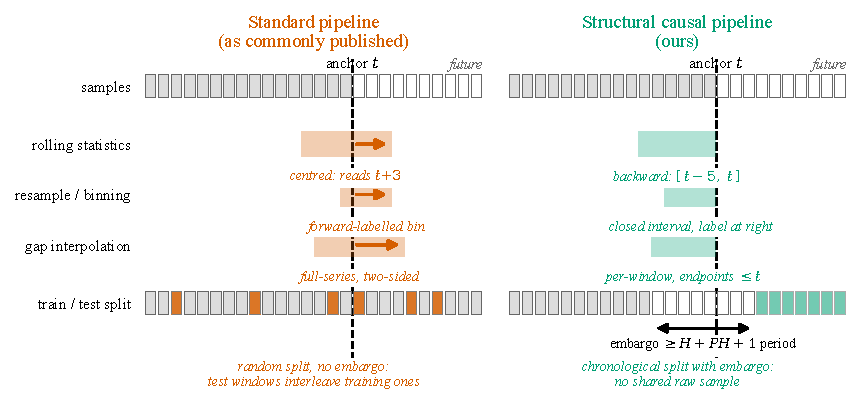
\includegraphics[width=0.9\textwidth]{fig2_anti_leakage_protocol.pdf}
  \caption{Where lookahead enters a CGM pipeline, and where it cannot. Left: the
  conventional arrangement, in which centred statistics, forward-labelled bins
  and whole-series interpolation all read past the anchor, and a random split
  interleaves test windows with training ones. Right: invariants I1--I5. Bands
  are drawn to scale in sample units, so a band crossing the anchor really does
  read the future.}
  \label{fig:leakage}
\end{figure*}

\section{Methodological Architecture}
\label{sec:method}

\subsection{Dual-Branch Causal Trunk with Gated Cross-Attention}

The architecture is drawn in Figure~\ref{fig:arch}
(Appendix~\ref{app:methods}). CGM and auxiliary streams differ in noise characteristics, missingness pattern
and scale by orders of magnitude, so they receive separate temporal
convolutional trunks~\citep{bai2018empirical,oord2016wavenet} rather than an
early concatenation that would force one normalisation regime on all of them.
Both trunks are causal: each layer left-pads and trims, so the receptive field
at position $i$ covers only $[\,i - r + 1,\ i\,]$.

Fusion is a single-head cross-attention from CGM queries to auxiliary keys and
values, masked so that position $i$ attends only to auxiliary positions
$j \le i$. Auxiliary streams are informative at variable, state-dependent lags,
which is what attention buys over concatenation. Writing $h_{\text{cgm}}$ and
$h_{\text{aux}}$ for the two branch representations, $f$ for the attended
auxiliary summary, $g$ for a gate computed from $[h_{\text{cgm}}, f]$, and $m$
for per-sample auxiliary availability:
\begin{equation}
  h \;=\; h_{\text{cgm}} \;+\; \big(g \odot \mathrm{LN}(f)\big) \odot m .
  \label{eq:fusion}
\end{equation}
Here $g \in \mathbb{R}^{d}$ matches the hidden dimension of $h_{\text{cgm}}$ and
$m \in \{0,1\}$ broadcasts over it, so with $m = 0$ this is \emph{exactly}
$h_{\text{cgm}}$. This is an architectural identity, not a performance
guarantee: $h_{\text{cgm}}$ is trained jointly with the fusion path, so the
fused model with $m = 0$ is not the separately trained unimodal model.
The LayerNorm is applied to the fusion term only and without a learned bias,
because normalising the sum would destroy the magnitude information the residual
regression head needs.

\paragraph{Auxiliary validity is a set property, never a single channel.} A window
is auxiliary-valid when, somewhere in its history, \emph{any} observation mask
among the streams in use is set or a treatment channel in use (insulin,
carbohydrate), which carries no mask, is non-zero; reading it from
one channel collapses the multimodal model onto the unimodal one for any subject
lacking that sensor (Appendix~\ref{sec:appendix_aux_validity}).

\subsection{Multi-Horizon, Multi-Task Heads}

Following the multitask formulation of \citet{fang2026glucose}, the model shares
a temporal representation trunk before branching into a point-regression head and
a hypoglycemia head, so that one forward pass produces both outputs. The trunk
itself is not theirs and we do not claim it as a reproduction: the dual-branch
auxiliary fusion of Section~\ref{sec:method}, the causally masked cross-attention,
the per-horizon application of uncertainty weighting (they weight their two
tasks by learned uncertainty), the conformal layer and the adaptation stage are
this work's. Their multicentre cohort includes the OhioT1DM subjects we evaluate
on, at far larger scale. The inherited commitments are the shared-trunk
multitask structure and the soft-label treatment of the hypoglycemia boundary.
Their soft label is a risk-probability mapping with sample selection above a
threshold rather than a band, so Ablation~\ref{sec:ablation-e} sweeps our own
formulation and is not a comparison with theirs.

One head pair per horizon reads the shared trunk and fusion policy; only the
readout is horizon-specific. Thirty- and sixty-minute forecasting are the same
physiology at different lead times, so separate trunks would double the
parameters and halve the data each trunk sees for the rare hypoglycemic events.

Each regression head predicts a \emph{residual} from the last observed value,
$\hat{y} = \BG(t) + \Delta$: absolute-level regression scores well by echoing
its input, at a lag equal to the full horizon and no clinical value.

\subsection{Loss: Uncertainty Weighting and Clinical Asymmetry}

The regression and classification losses live on incompatible scales
(mg/dL$^2$ versus nats), so a hand-tuned $\lambda$ is fragile. We adopt the
functional form of homoscedastic uncertainty
weighting~\citep{kendall2018multitask}, one learned log-variance per task
\emph{per horizon}:
\begin{equation}
  \mathcal{L} \;=\; \sum_{i} \Big[ e^{-s_i} \mathcal{L}_i + \tfrac{1}{2} s_i \Big],
  \label{eq:kendall}
\end{equation}
where $i$ ranges over the $2K$ task-horizon pairs ($K = 2$ horizons, at 30 and
60~min). Sharing a weight across
horizons would let the easier horizon dominate the gradient while the harder one
degrades toward predicting the mean.

\paragraph{A scaling heuristic, not a derivation.} We follow
\citet{kendall2018multitask} to combine losses on disparate scales, but our
asymmetric-Huber and soft-label terms do not meet its likelihood premises
(Gaussian for regression, a scaled softmax for classification):
Equation~\ref{eq:kendall} is a parameterisation of a hyperparameter, not an
uncertainty model (Appendix~\ref{sec:appendix_kendall}).
Ablation~\ref{sec:ablation_a} cannot separate it from a fixed $\lambda = 1$ at
one seed ($\NumAblAKendallEdgeHThirty$~PR-AUC at $\PH = 30$, comparable to
seed-to-seed variation), so its value is
one fewer knob per cohort, not accuracy.


The regression term is a weighted Huber loss whose weights encode the clinical
asymmetry. With a smooth ramp
$\rho(y) = \sigma\!\left((70 - y)/\tau\right)$, $\tau = 10$~mg/dL, marking how
hypoglycemic the \emph{reference} is,
\begin{equation}
  w(\hat{y}, y) \;=\; 1 + (\kappa - 1)\,\rho(y)\,\ind[\hat{y} > y],
  \label{eq:asym}
\end{equation}
and $\mathcal{L}_{\text{reg}} = \sum_n w_n \ell_\delta(\hat{y}_n, y_n) /
\sum_n w_n$ for the Huber loss $\ell_\delta$ at $\delta = 10$~mg/dL. The
penalised direction is over-prediction of a low, which is the
direction that produces zone~D. The ramp is smooth rather than a hard indicator
at 70 for the same reason the classification labels are soft: CGM error is on
the order of 10~mg/dL, so a hard cut places a discontinuity precisely where the
true class is least certain. Normalising by $\sum_n w_n$ keeps the loss on a
fixed scale, so raising $\kappa$ does not silently rescale the learned task
weights of Equation~\ref{eq:kendall}. At $\kappa = 1$ the mechanism is an exact
no-op.

\subsection{Mondrian Conformal Prediction}
\label{sec:conformal}

Split conformal calibrates one quantile $\hat{q}$ of the absolute residuals and
emits $[\hat{y} \pm \hat{q}]$, valid marginally. We instead partition the glucose
axis into the three clinical zones $\zone{1} = [0, 70)$, $\zone{2} = [70, 180]$,
$\zone{3} = (180, \infty)$ and calibrate a separate $\hat{q}_k$ inside each. The
taxonomy is a function of the \emph{target}, which is unknown at inference, so
assigning the zone from $\hat{y}$ would fail hardest where it matters: a true
60~mg/dL read as 100 would receive the narrow euglycemic width. We therefore emit
the convex hull of the label-conditional region
\begin{equation}
  \mathcal{C}(\hat{y}) \;=\;
  \operatorname{conv} \bigcup_{k=1}^{3}
    \big\{\, y \in \zone{k} \;:\; |y - \hat{y}| \le \hat{q}_k \,\big\},
  \label{eq:mondrian}
\end{equation}
where zone $k$ contributes iff
$\operatorname{dist}(\hat{y}, \zone{k}) \le \hat{q}_k$. \emph{The emitted interval
covers $y$ whenever the oracle interval, the one built from the true and
unobservable zone, would have.} Appendix~\ref{sec:appendix_conformal_method}
gives the two-line proof, the boundary convention and the small-stratum
fallback.

\section{Experimental Setup}
\label{sec:setup}

\subsection{Cohort and Protocol}

We use OhioT1DM~\citep{marling2018ohiot1dm,marling2020ohiot1dm}: twelve
individuals with type~1 diabetes on insulin pump therapy, six released in 2018
wearing a Basis Peak and six in 2020 wearing an Empatica Embrace, each with
approximately eight weeks of five-minute CGM alongside insulin, meal and
wearable streams. The released split is temporal and \emph{within} patient:
every subject appears in both \texttt{train/} and \texttt{test/}. We keep it.
Feeding these windows to a patient-wise cross-validation would substitute a
different and non-comparable protocol while appearing to report the benchmark.

With $H = 24$ steps (120~min) and horizons $\{30, 60\}$~min at stride~1 the
cohort yields \NumFitWindows{} fit, \NumValWindows{} model-selection validation,
\NumCalibWindows{} disjoint conformal calibration, and \NumTestWindows{} test windows,
separated by invariant~I5's embargo. The split is four-way because split conformal 
assumes the predictor is fixed independently of the calibration rows, so the calibration 
slice is disjoint from and embargoed from the validation slice, as from test. All are 
chronological tails of each subject's training file, never random samples.

\subsection{Baselines}
\label{sec:baselines}

All arms are fitted on the fit split, early-stopped on the validation split,
conformal-calibrated on the disjoint calibration split, and scored on the test
split through one shared metric path. A baseline compared under different conditions 
is not a baseline.

\textbf{Persistence} predicts $\BG(t{+}\PH) = \BG(t)$; it is the floor every
model must clear, and its failure mode is horizon-dependent in a way RMSE does not
expose.
\textbf{Ridge-AR} is a direct multi-step penalised linear autoregression on the
24 lags, one fit per horizon, targeting the residual from the last observed
value. Its ridge penalty is fixed at $\alpha = 10$ rather than tuned, and the fit is
well conditioned enough that the choice barely moves the forecast. 
\textbf{ARIMA($4,1,0$)}~\citep{box2015time} is fitted per
subject by conditional maximum likelihood on that subject's own training series
and applied causally per window. Its order is fixed a priori ($p = 4$, $d = 1$, $q = 0$, the last because an MA
term is not well defined on a 24-sample window under this protocol,
Appendix~\ref{sec:appendix_baselines}). Neither classical baseline is
hyperparameter-tuned; Ablation~\ref{sec:ablation_f} quantifies the larger
handicap, target misspecification.
\textbf{LightGBM}~\citep{ke2017lightgbm} uses 43 causal lag features
with one model pair per horizon. 
\textbf{Dilated LSTM} is a unidirectional
recurrent trunk on CGM alone.

Three arms (persistence, Ridge-AR and ARIMA) have no classification head and
receive a hypoglycemia score of $\sigma\!\left((70 - \hat{y})/\tau\right)$, a
strictly monotone map of the forecast that invents nothing. It does ask them an
uneven question: a level forecast at $t{+}\PH$ is blind to a nadir at $t{+}20$
that recovers by $t{+}30$, so their classification columns are lower bounds
(Appendix~\ref{sec:appendix_sigmoid}). LightGBM and both neural arms fit a
classifier on the nadir label itself and are unaffected.

\subsection{Metrics}

Regression: RMSE, MAE, MARD, and a cross-correlation \textbf{time lag}, the shift
that maximises correlation between prediction and truth. Persistence scores a lag
of exactly $\PH$; an anticipatory model scores less. The lag is computed per
contiguous segment, because on a shuffled evaluation set one array step is not one
sampling period.

Clinical safety: the Clarke~\citep{clarke1987evaluating} and
Parkes~\citep{parkes2000new} error grids
(Appendix~\ref{sec:appendix_grids}).

Forewarning: PR-AUC, sensitivity at 5\% and 10\% FPR, and two metrics in the
unit the patient experiences. \textbf{False alarms per day} (FAPD) counts alarm
\emph{episodes}, not samples: a device latches while the score stays above
threshold, so a 40-minute spurious excursion is one beep where a naive count
reports eight, and an
episode containing any true positive is a true alarm that started early rather
than an additional false one. \textbf{Warning lead time} is the gap between the
earliest valid alert and the event's onset, its first reading below 70~mg/dL,
where an alert at $a$ is valid for an onset at $s$ exactly when
$a \in [s - P,\ s - 1]$ and the reading at $a$ is not already below
70~mg/dL, derived from the label definition rather than assumed; an ``alert''
at the onset itself does not count. Lead time to the nadir, which is longer by
construction, is reported only where a table says so.

Uncertainty: empirical coverage and mean width at $\alpha = \NumAlpha$,
marginal and stratified by clinical band.

\section{Results and Discussion}
\label{sec:results}

\subsection{Benchmark Comparison}

\begin{table*}[t]
\centering
\small
\setlength{\tabcolsep}{4pt}
\caption{OhioT1DM test split, $\PH = 30$~min: mean $\pm$ sd over 5 training seeds. Alarm thresholds are fitted on the calibration split and applied unchanged to test. PR-AUC (onset) excludes anchors that are below 70~mg/dL now or in the preceding 30~min. Onset lead is minutes from the first valid alert to the first reading below 70. FAPD@5\% counts false alarm episodes under the default alarm policy: an episode lasts while the score stays above threshold, with no merging across gaps and a minimum duration of one reading (5~min); Appendix~\ref{sec:appendix_latching} varies both. Classical arms and LightGBM are deterministic (sd 0).}
\label{tab:sota_multiseed_ph30}
\resizebox{\ifdim\width>\linewidth\linewidth\else\width\fi}{!}{%
\begin{tabular}{lrrrrrrr}
\toprule
Arm & RMSE & PR-AUC & PR-AUC (onset) & Se@5\% (cal.) & FAPD@5\% & Onset lead & D+E \\
\midrule
Persistence & 23.29 $\pm$ 0.00 & 0.832 $\pm$ 0.000 & 0.333 $\pm$ 0.000 & 0.933 $\pm$ 0.000 & 1.16 $\pm$ 0.00 & 23.7 $\pm$ 0.0 & 272 $\pm$ 0 \\
Ridge-AR & 20.05 $\pm$ 0.00 & 0.829 $\pm$ 0.000 & 0.416 $\pm$ 0.000 & 0.964 $\pm$ 0.000 & 2.99 $\pm$ 0.00 & 26.4 $\pm$ 0.0 & 351 $\pm$ 0 \\
ARIMA(4,1,0) & 21.09 $\pm$ 0.00 & 0.856 $\pm$ 0.000 & 0.405 $\pm$ 0.000 & 0.957 $\pm$ 0.000 & 2.05 $\pm$ 0.00 & 25.8 $\pm$ 0.0 & 187 $\pm$ 0 \\
LightGBM & 18.92 $\pm$ 0.00 & 0.841 $\pm$ 0.000 & 0.460 $\pm$ 0.000 & 0.968 $\pm$ 0.000 & 2.90 $\pm$ 0.00 & 27.1 $\pm$ 0.0 & 270 $\pm$ 0 \\
Dilated LSTM (CGM) & 19.35 $\pm$ 0.15 & 0.863 $\pm$ 0.008 & 0.435 $\pm$ 0.029 & 0.964 $\pm$ 0.004 & 2.61 $\pm$ 0.21 & 26.4 $\pm$ 0.2 & 172 $\pm$ 6 \\
CausalCGM-MT (CGM) & 19.28 $\pm$ 0.09 & 0.863 $\pm$ 0.004 & 0.414 $\pm$ 0.028 & 0.958 $\pm$ 0.006 & 2.64 $\pm$ 0.19 & 26.0 $\pm$ 0.6 & 195 $\pm$ 23 \\
CausalCGM-MT (fusion) & 18.76 $\pm$ 0.14 & 0.863 $\pm$ 0.009 & 0.437 $\pm$ 0.032 & 0.953 $\pm$ 0.003 & 2.47 $\pm$ 0.20 & 26.2 $\pm$ 0.2 & 197 $\pm$ 28 \\
CausalCGM-MT + LoRA (r=4) & 21.62 $\pm$ 0.34 & 0.670 $\pm$ 0.065 & 0.247 $\pm$ 0.041 & 0.808 $\pm$ 0.068 & 1.78 $\pm$ 0.14 & 21.7 $\pm$ 1.1 & 341 $\pm$ 33 \\
\bottomrule
\end{tabular}}
\end{table*}


Table~\ref{tab:sota_multiseed_ph30} reports the official test split at
$\PH = 30$~min over $\NumMSSeeds$ seeds. Table~\ref{tab:multiseed_diffs_ph30}
gives subject-cluster bootstrap CIs ($\NumMSBoot$ draws), and
Appendix~\ref{sec:appendix_benchmarks} gives the single-seed tables with every
metric. Alarm thresholds are fitted on the calibration split at a 5\% target
and applied unchanged to test. The realised false-positive rate is
$\NumMSRealFPRMinPct$--$\NumMSRealFPRMaxPct\%$ across the non-personalised arms
at $\PH = 30$.

The three neural arms do not separate on forewarning. Over seeds, the fusion
PR-AUC differs from the CGM-only and LSTM PR-AUCs by
$\NumMSDiffCGMOnlyPRAUCHThirty$ and $\NumMSDiffLSTMPRAUCHThirty$, and both CIs
span zero. Restricted to anchors that are not already hypoglycemic, LightGBM's
PR-AUC ($\NumMSLGBMPRAUCOnsetHThirtyMean$) exceeds fusion's
($\NumMSFusionPRAUCOnsetHThirtyMean$); the CI on that difference also spans
zero. Lead time is measured to onset, the first reading below 70~mg/dL. It is
$\NumMSFusionOnsetLeadHThirtyMean$~min for fusion against
$\NumMSPersistOnsetLeadHThirtyMean$ for persistence.

\paragraph{Point accuracy and what drives it.} Fusion lowers RMSE relative to
the CGM-only network: the fusion-minus-CGM-only difference is
$\NumMSDiffCGMOnlyRMSEHThirty$~mg/dL at 30~min (95\% CI
$[\NumMSDiffCGMOnlyRMSEHThirtyLo, \NumMSDiffCGMOnlyRMSEHThirtyHi]$) and
$\NumMSDiffCGMOnlyRMSEHSixty$ at 60~min
($[\NumMSDiffCGMOnlyRMSEHSixtyLo, \NumMSDiffCGMOnlyRMSEHSixtyHi]$). Ablation~C
attributes the gain to treatment inputs: adding insulin and carbohydrate alone
changes RMSE by $\NumAblCTreatTwentyRMSEHThirty$ (2020) and
$\NumAblCTreatEighteenRMSEHThirty$ (2018) at 30~min, while wearable-only arms
are null or worse at that horizon. Against LightGBM the difference is
$\NumMSDiffLGBMRMSEHThirty$~mg/dL
($[\NumMSDiffLGBMRMSEHThirtyLo, \NumMSDiffLGBMRMSEHThirtyHi]$), which we do not
claim as a lead. On MetaboNet the gain over CGM-only replicates, smaller
($\NumMetaboFusionDeltaRMSE$~mg/dL; Appendix~\ref{sec:metabonet}).

\paragraph{Clarke zone D/E errors come from the loss.} Over seeds fusion makes
$\NumMSFusionDEHThirtyMean \pm \NumMSFusionDEHThirtySD$ zone D/E errors against
LightGBM's $\NumMSLGBMDEHThirtyMean$
($\NumMSDiffLGBMDEHThirty$, CI $[\NumMSDiffLGBMDEHThirtyLo,
\NumMSDiffLGBMDEHThirtyHi]$). Within the single-seed ablation budget, the same
fusion model makes $\NumKappaOneDE$ at $\kappa = 1$ and $\NumKappaThreeDE$ at
$\kappa = 3$ (Ablation~B), so the gap tracks the asymmetric loss, which
LightGBM lacks; the two budgets are not compared with each other. Against arms sharing the loss it is not resolved.

\paragraph{Persistence is a strong classifier.} Persistence reaches PR-AUC
$\NumPersistPRAUCHThirty$ because ``already low'' predicts the nadir; the
onset-only PR-AUC removes that floor.

\subsection{Ablation B: The Asymmetry Trade-Off}

\begin{figure*}[t]
  \centering
  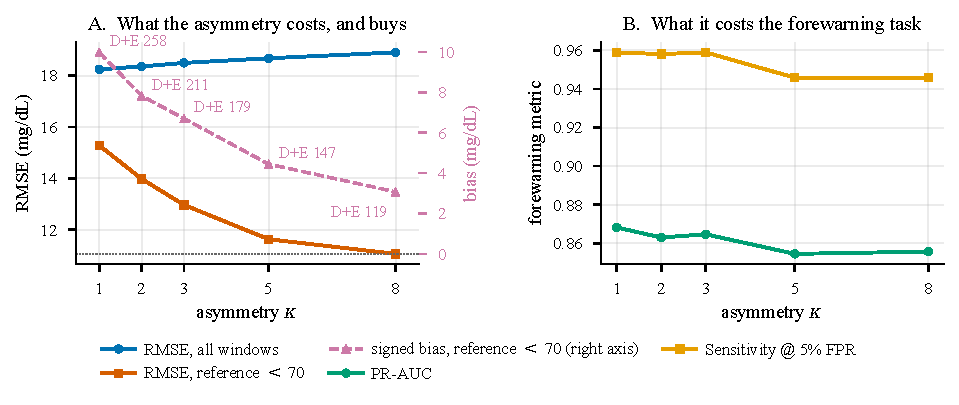
\includegraphics[width=\textwidth]{fig5_ablation_tradeoffs.pdf}
  \caption{The asymmetric hypoglycemia cost, official OhioT1DM test split,
  $\PH = 30$~min. (A)~Raising $\kappa$ trades overall RMSE for accuracy and
  signed bias below 70~mg/dL, with Clarke D+E counts annotated. (B)~It also
  costs forewarning discrimination. There is no free operating point, and $\kappa$ 
  is not tuned to any objective.}
  \label{fig:tradeoff}
\end{figure*}

This result is a trade rather than an improvement: raising $\kappa$ buys accuracy and
signed bias below 70~mg/dL, and Clarke zone D+E errors, and pays for all of it in
overall RMSE and forewarning discrimination
(Appendix~\ref{sec:appendix_ablation_b}, Table~\ref{tab:ablation_b_asymmetry_ph30}; Figure~\ref{fig:tradeoff}). At the
repository default $\kappa = 3$ that costs $\NumKappaThreeRMSECostPct\%$ overall
RMSE and $\NumKappaThreePRAUCDrop$ PR-AUC. We claim the direction, not an
optimum: zone D+E counts, RMSE below 70~mg/dL and hypoglycemic bias fall
monotonically in $\kappa$ while overall RMSE rises; PR-AUC is not monotone, and
its range is comparable to seed-to-seed variation. Which point on the curve is acceptable is a clinical
judgement, and Figure~\ref{fig:tradeoff} rather than any single $\kappa$ is the
result (Appendices~\ref{sec:appendix_clarke},~\ref{sec:appendix_ablation_b}).

\subsection{Ablation D: What Lookahead Bias Buys}

\begin{table*}[t]
\centering
\small
\setlength{\tabcolsep}{4pt}
\caption{Ablation D: what lookahead bias buys (PH = 30 min). Arms are \emph{not} scored on the same test set: changing the split is the flaw being measured.}
\label{tab:ablation_d_leakage_ph30}
\resizebox{\ifdim\width>\linewidth\linewidth\else\width\fi}{!}{%
\begin{tabular}{lrrrrrrr}
\toprule
Arm & RMSE & MAE & PR-AUC & Se@5\% & A+B (\%) & Lag (min) & $n$ test \\
\midrule
Strict causal pipeline (ours) & 18.49 & 12.78 & 0.865 & 0.959 & 99.36 & 20.0 & 28335 \\
+ unembargoed random split & 18.73 & 12.75 & 0.878 & 0.938 & 99.19 & -- & 29932 \\
+ full-series interpolation \& centred features & 14.24 & 9.02 & 0.943 & 0.988 & 99.59 & -- & 37704 \\
\bottomrule
\end{tabular}}
\end{table*}


Only the pipeline varies; architecture, loss, optimiser, seed, horizons and
channel layout are fixed. The arms are not scored on the same test set, because
changing the split is the flaw, so the table answers how much better a reported
number looks. All ablations share one budget, lighter than
Table~\ref{tab:sota_ph30}'s, and compare only to each other.

For this model and budget, an unembargoed random split \emph{on its own}
changes little at $\PH = 30$: measured RMSE goes from $\NumLeakSplitRMSEStrict$
to $\NumLeakSplitRMSELeaky$~mg/dL, $\NumLeakSplitRMSEIncreasePct\%$ higher
than under the strict pipeline, and PR-AUC rises by $\NumLeakSplitPRAUCIncrease$.
At $\PH = 60$ it is not negligible: measured RMSE is
$\NumLeakSplitRMSEReductionPctHSixty\%$ lower than under the strict pipeline.
Adding whole-series interpolation and centred rolling statistics changes the
picture: measured RMSE falls from $\NumLeakNaiveRMSEStrict$ to
$\NumLeakNaiveRMSELeaky$~mg/dL, $\NumLeakNaiveRMSEReductionPct\%$ lower than
under the strict pipeline, and PR-AUC rises from $\NumLeakNaivePRAUCStrict$ to
$\NumLeakNaivePRAUCLeaky$ (by $\NumLeakNaivePRAUCIncrease$); at $\PH = 60$,
measured RMSE is $\NumLeakNaiveRMSEReductionPctHSixty\%$ lower and PR-AUC
$\NumLeakNaivePRAUCIncreaseHSixty$ higher. At both horizons this lowers measured
RMSE and raises PR-AUC by more than the split alone does. It is the same model,
so the gap is optimistic bias in apparent performance, not a better forecaster. The costly flaws here are in feature and label construction, and they
survive a disjointness assertion untouched. The mechanism is generic to windowed
forecasting, but we measured it only on CGM; its size elsewhere is a hypothesis
(Appendix~\ref{sec:appendix_ablation_d}).

\subsection{Few-Shot Personalisation: A Negative Result}

The OhioT1DM protocol is temporal and \emph{within} patient, so per-subject
adaptation is the natural question, and the answer is negative. Adapting the
population model to each of $\NumPersSubjects$ subjects from a
$\NumPersPrefixHours$-hour prefix of its own training file makes the model worse
at the default budget of $\NumPersDefaultSteps$ gradient steps in every mode tested (BatchNorm
recalibration, LoRA at ranks 4 and 8 with an
L2-SP anchor, head-only and full fine-tuning): BatchNorm adaptation alone costs
$\NumPersBNAdaptRMSEDelta$~mg/dL RMSE ($p_{\text{Holm}} = \NumPersBNAdaptRMSEP$),
and for LoRA at rank~4 the damage grows with the number of adaptation steps. Very
short head-only budgets nominally lower RMSE
($\NumPersHeadOnlyStepsTenDelta$~mg/dL after ten steps; unadjusted 95\% CI
$[\NumPersHeadStepsTenCILow, \NumPersHeadStepsTenCIHigh]$, $p = \NumPersHeadStepsTenP$,
no multiplicity correction) without raising mean PR-AUC at any budget tested
(Appendix~\ref{sec:personalisation}). The design limits
what this shows. The prefix lies inside the population model's own training
split, so adaptation adds no new information, and no mode uses held-out early
stopping. The result is that this recipe degrades the model, on OhioT1DM and on
unseen MetaboNet subjects alike; it does not separate scarce data from
over-adaptation as the cause (Appendix~\ref{sec:personalisation}).


\section{Uncertainty via Conformal Prediction}
\label{sec:conformal_results}

Split conformal attains $\NumSplitCov$ marginal coverage at $\alpha = \NumAlpha$,
as the theory requires. Its conditional behaviour runs opposite to the usual
expectation. Hypoglycemic-band coverage is $\NumSplitHypoCov$, so the
constant-width interval \emph{over}-covers there. The reason is the asymmetric
loss: it has already pulled hypoglycemic predictions toward the truth, so their
residuals are smaller than the model's overall.

Mondrian conformal equalises coverage across zones and narrows the
hypoglycemic interval. It undercovers the severe tail, however. Below
54~mg/dL its coverage is $\NumBootMondrianSevereMin$--$\NumBootMondrianSevereMax$
across $\NumBootSeeds$ seeds. On every seed it falls below the nominal 0.90 in
$\NumBootMondrianBelowMinPct$--$\NumBootMondrianBelowMaxPct\%$ of
$\NumBootDraws$ block-bootstrap resamples of the calibration split
(Appendix~\ref{sec:appendix_conformal_results}). The $<54$ cell is a sub-band of
the hypoglycemic stratum, and the narrower stratum quantile undercovers its
extreme tail.

Normalised conformal scales one pooled quantile by $\sigma$, the mean absolute
glucose change over the last 30 minutes of the input window; $\sigma$ is a
fixed proxy, not a fitted model. It does not consistently repair the severe
tail. It exceeds split conformal in the severe cell on
$\NumBootNormBeatsSplitSeeds$ of $\NumBootSeeds$ seeds, and severe-cell coverage
varies more between training seeds (split
$\NumBootSplitSevereMin$--$\NumBootSplitSevereMax$, normalised
$\NumBootNormSevereMin$--$\NumBootNormSevereMax$) than between calibration
draws. We therefore make no recommendation between split and normalised
conformal on this benchmark. The cell holds $\NumBootSevereN$ autocorrelated
test windows, and calibration and test windows are temporally dependent. All
three guarantees therefore hold only approximately. Adaptive conformal
inference~\citep{gibbs2021adaptive} targets that setting and is untested here.

\section{Limitations and Ethical Considerations}

\paragraph{Cohort size and what twelve subjects support.} Twelve subjects is the
standard OhioT1DM benchmark and it is small. We keep the released within-patient
split for comparability and claim no generalisation beyond adults on pump
therapy in the United States. Benchmark arms are reported over
$\NumMSSeeds$ seeds with subject-level bootstrap CIs; the ablations and the
personalisation study remain single-seed and are read as directions. The
MetaboNet replication is single-seed, and $\NumMetaboCLSubjPct\%$ of its
subjects come from studies of automated insulin delivery
(Appendix~\ref{sec:metabonet}).
Our baselines are standard model families; no published CGM forecasting system
is reproduced. The 2018/2020
releases use disjoint sensor sets, leaving some modality arms untrainable
(Appendix~\ref{sec:appendix_aux_validity}).

\paragraph{Real-world logging.} Carbohydrate and bolus logging is often delayed
or omitted in free-living use, and our benchmark uses research-grade logs. The
fusion gain comes from those inputs, so it should shrink when logging degrades;
we have not measured that.

\paragraph{Conditional coverage in the severe tail.} No construction tested here
certifies coverage below 54~mg/dL: Mondrian undercovers it consistently, and
split and normalised coverage there move with the training seed. Device-grade
certification of that tail needs far more data than the $\NumBootSevereN$ test
windows below 54~mg/dL that this benchmark provides.

\paragraph{Regulatory boundary.} Under FDA guidance on clinical decision
support software, software that analyses CGM signals or issues time-critical
alarms is a device function~\citep{fda2026cds}, so a hypoglycemia forewarning
system is likely within device regulation even though it does not dose. This is
a research model, not a validated device. Neither the asymmetric loss nor the
conformal intervals change that, and $\kappa$ encodes a clinical judgement
belonging to clinicians and patients rather than a configuration default.

\paragraph{Alarm burden as an equity issue.} False-alarm burden is uneven: users
with more variable glycemia receive more alerts and, as alarm fatigue suggests,
may come to respond to them less, so we
report FAPD at a fixed operating point rather than an aggregate AUC, making that
burden visible. The personalisation finding is not evidence that
personalisation cannot work: adaptation used at most 48 hours of data, inside
the population model's training split on OhioT1DM, without held-out early
stopping.

\section{Conclusion and Reproducibility}

(1)~\textbf{Data hygiene.} For this model and budget, whole-series
interpolation and centred statistics inflate apparent performance (lower
measured RMSE, higher PR-AUC than a strict pipeline) more than an unembargoed
random split does, at both horizons. (2)~\textbf{Clinical asymmetry.}
$\kappa$ trades accuracy for fewer Clarke zone~D/E errors.
(3)~\textbf{Inputs over architecture.} The fusion gain comes from insulin and
carbohydrate inputs; gradient-boosted trees match the network on RMSE and PR-AUC.
(4)~\textbf{Conformal tails.} Mondrian conformal undercovers $<54$~mg/dL events,
and no alternative tested certifies that tail.

% Back matter, before the bibliography; the appendices follow on a new page.
\acks{I thank my good friend Liam Chandra for his invaluable insights into
common points of failure in machine learning contexts, Andrew Burden for
teaching me how to be a rigorous scientist, and my friends and family for
supporting me in my efforts to learn about the world.}

\section*{LLM Usage Disclosure}
The author of this paper used LLMs as an adversarial auditor. Additionally, the
author used LLMs to make sure that all information in the paper comes from
macros that were built from the results files. The author also used LLMs to
draft and revise code and to revise manuscript wording. Any ideas, results, and
figures, are entirely the author's responsibility.

\section*{Competing Interests}
The author declares no competing financial or non-financial interests.

\section*{Compute Resources}
Every model in this paper is trained and evaluated on CPU; no GPU is used at any
stage, and none is required to reproduce the results. The benchmark, ablation
and personalisation stages, including the $\NumMSSeeds$-seed benchmark sweep,
run from a single driver (\texttt{reproduce\_all\_paper\_results.sh}) in hours on
a workstation CPU; the MetaboNet study, run separately
(\texttt{run\_metabonet\_benchmarks.py}), took $\NumMetaboComputeHours$~hours of
summed arm-fold wall clock. The serving measurements of
Section~\ref{sec:edge} are taken on an \NumEdgeCPU{} ($\NumEdgeCores$ cores).

% \bibliographystyle is set to plainnat by jmlr.cls; re-issuing it here
% makes BibTeX abort with "Illegal, another \bibstyle command".
\bibliography{references}

% Appendices start on a new page after the bibliography.
\clearpage
\appendix

% Appendix A -- methodology and implementation notes lifted out of the 8-page
% body. Every subsection here is pointed at by a \ref from Sections 1-4.
\section{Methodological and Implementation Details}
\label{app:methods}

\begin{figure*}[t]
  \centering
  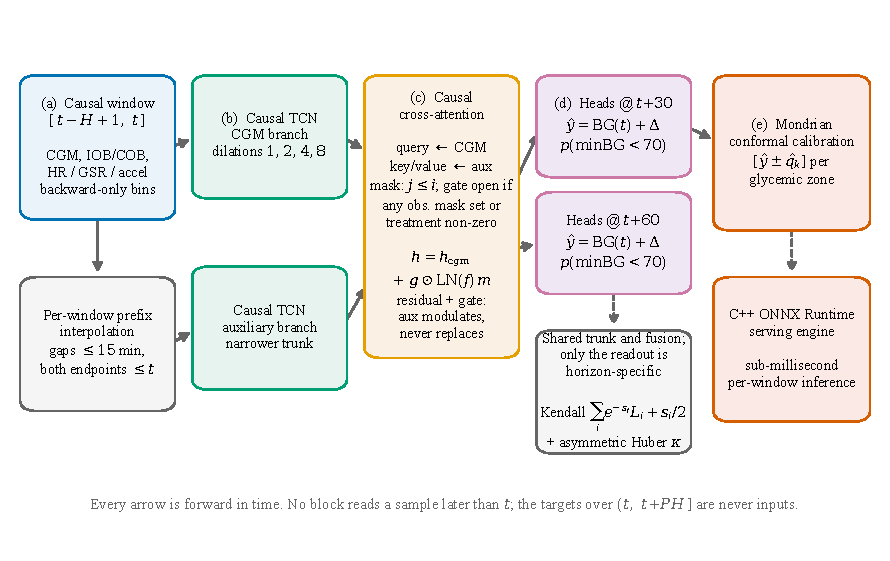
\includegraphics[width=0.9\textwidth]{fig1_architecture.pdf}
  \caption{CausalCGM-MT. (a)~A closed causal window feeds (b)~two causal TCN
  trunks, fused by (c)~cross-attention masked both temporally and by auxiliary
  availability, read out by (d)~per-horizon residual regression and nadir
  classification heads under a Kendall-weighted objective with the asymmetric
  hypoglycemia penalty, and deployed through (e)~Mondrian conformal calibration
  and a C++ ONNX engine. No block reads a sample later than $t$.}
  \label{fig:arch}
\end{figure*}

\subsection{Scope and Relation to Prior Work}
\label{sec:appendix_scope}

A user's tolerance for spurious alerts is finite, and the literature
systematically under-weights it. Alarm fatigue is a documented failure mode of
clinical monitoring in general~\citep{cvach2012monitor} and of diabetes devices
in particular~\citep{shivers2013turn}: users who receive too many spurious alerts
become less likely to respond to them, and an alert that is ignored protects
no one. A forewarning
system therefore has to be evaluated in the unit the patient experiences: false
alarms per day at a usable operating point, and how much warning a true alert
actually provides, not only in the units that are convenient to compute.

The multitask framing this paper builds on is not ours. \citet{fang2026glucose}
introduced MT-HypoNet, which couples continuous glucose forecasting to
hypoglycemia forewarning through a shared representation, and validated it on a
retrospective multicentre cohort of 1{,}662 patients spanning type~1 and type~2
diabetes, together with a prospective perioperative cohort of 36 further
patients, a scale of clinical evidence this work does not
approach. The statistically guided soft-label strategy for the hypoglycemia
boundary is likewise theirs. What we contribute is orthogonal to that evidence
and complementary to it. More specifically, the multitask formulation is adopted,
and the questions we ask are whether it can be trained without lookahead leakage, whether its
forewarning score can be given conditional coverage guarantees, and whether the
resulting artefact can be served with verified train/serve parity. Those are
engineering and evaluation questions, and answering them on a twelve-subject
public benchmark is a different exercise from establishing clinical
generalisation on 1{,}662 patients.

\subsection{The Auxiliary-Validity Defect}
\label{sec:appendix_aux_validity}

A window counts as
auxiliary-valid when, somewhere in its history, \emph{any} observation mask
among the streams in use is set or a mask-free treatment channel in use
(delivered insulin, insulin or carbohydrate on board, logged carbohydrate) is
non-zero. An earlier version read validity from the heart-rate mask alone. The 2020
OhioT1DM subjects wore an Empatica device that reports no heart rate, so that
channel is identically zero across all of their windows, the cross-attention was
fully masked, and the ``multimodal'' model was the CGM-only model for half the
cohort while continuing to report itself as multimodal. The same defect collapsed every modality-ablation arm that excluded
heart rate onto bit-identical numbers. We record the fraction of timesteps at
which the gate is open in every results file, and warn at training time when it
is zero.

\subsection{Note on the Kendall Weighting}
\label{sec:appendix_kendall}

Kendall et al.\ derive Equation~\ref{eq:kendall} as a Gaussian
maximum-likelihood objective in which $e^{-s_i}$ is a reciprocal noise variance
with a defined unit. Two departures are worth stating. The first is
presentational: under $s_i = \log \sigma_i^2$ their objective is
$\tfrac{1}{2}e^{-s_i}\mathcal{L}_i + \tfrac{1}{2}s_i$, and we drop the
$\tfrac{1}{2}$ on the loss term. A uniform factor on every task rescales the
whole objective and is absorbed by the learning rate, leaving the minimiser in
$s_i$ unchanged, so Equation~\ref{eq:kendall} is their objective up to that
constant. The second is substantive: neither of our terms meets the Gaussian
premise. The regression
loss is an asymmetric Huber whose weights depend on the reference value
(Equation~\ref{eq:asym}), so it is not the log-likelihood of any fixed noise
model and its implied density changes with $\kappa$; the classification loss is
a soft-label cross-entropy, whose corresponding derivation gives a different
form again. Treating the $s_i$ as commensurable uncertainties across the two is
therefore an analogy, not a probabilistic identity, and we do not claim the
learned $s_i$ estimate anything physical.

What the form does provide is a stable, scale-free way to combine terms whose
magnitudes differ by orders of magnitude and drift during training, with a
$\tfrac{1}{2} s_i$ penalty that stops the optimiser from driving either weight
to zero. Section~\ref{sec:ablation_a} measures this against a fixed
$\lambda = 1$ and finds the difference small and horizon-dependent. Read
Equation~\ref{eq:kendall}, then, as a well-behaved parameterisation of a
hyperparameter rather than a principled uncertainty model: a reader who prefers
the fixed-$\lambda$ arm loses little, and the value of the learned form is that
it removes a knob that would otherwise need re-tuning per cohort, horizon set
and class prior.

\subsection{Conformal Construction: Proof and Conventions}
\label{sec:appendix_conformal_method}

\paragraph{Zone conventions.} The brackets of
$\zone{1} = [0, 70)$, $\zone{2} = [70, 180]$, $\zone{3} = (180, \infty)$ follow
the clinical convention: both 70 and 180 lie inside the euglycemic band, so
$\zone{1} \cup \zone{2} \cup \zone{3} = [0, \infty)$ with the three pairwise
disjoint. In other words, every glucose value belongs to exactly one zone,
including the boundaries themselves. The same convention is implemented in
\texttt{clinical\_stratum}, where a non-finite value returns no stratum at all
rather than defaulting into $\zone{2}$.

\paragraph{Why the zone cannot be read from $\hat{y}$.} The taxonomy is a
function of the \emph{target}, which is unknown at inference. Mondrian conformal
is exactly valid for an observable taxonomy; assigning the zone from $\hat{y}$
and applying that zone's quantile is a heuristic that fails hardest where it is
needed: a true 60~mg/dL that the model reads as 100 receives the narrow
euglycemic width. Equation~\ref{eq:mondrian} instead emits the convex hull of the
label-conditional region, where zone $k$ contributes iff
$\operatorname{dist}(\hat{y}, \zone{k}) \le \hat{q}_k$.

\paragraph{The oracle-coverage guarantee.} This yields a two-line proof: if the true $y$ lies in $\zone{k}$ with
$|y - \hat{y}| \le \hat{q}_k$, then
$\operatorname{dist}(\hat{y}, \zone{k}) \le |y - \hat{y}| \le \hat{q}_k$, so zone $k$
is reachable and the emitted half-width is at least $\hat{q}_k$; hence $y$ is
covered. \emph{The emitted interval covers $y$ whenever the oracle interval, the
one built from the true and unobservable zone, would have.} A stratum with fewer
than $\lceil (1-\alpha)/\alpha \rceil$ calibration points cannot certify the
level at all and falls back to the pooled quantile with an explicit log record,
carrying the marginal guarantee rather than a conditional one.

\subsection{Deployment Path and Train/Serve Parity}
\label{sec:appendix_deployment}

The trained network is exported to ONNX behind a numerical-parity and causality
gate, and served by a standalone C++ ONNX Runtime~\citep{onnxruntime} binary with
no Python in the loop. Feature construction is reimplemented in C++ and verified
against the Python path element by element, because a graph-level parity check
cannot see it: a divergence in the hand-written feature code is train/serve skew,
in which the deployed model receives different inputs from the ones it was
trained on while every export test still passes.
The C++ path is verified for the CGM channels only: the runner implements no
auxiliary feature path and serves a fusion graph with its auxiliary input zeroed
and the presence gate closed, which is exactly the CGM-only computation, and
the element-wise parity check runs on a CGM-only demonstration graph. Serving
the fusion model with live auxiliary streams is not implemented.
Section~\ref{sec:edge} reports what that stack costs to run. We describe it as a
deployment path rather than as an embedded implementation: the binary targets a
general-purpose CPU, and porting it to constrained silicon is out of scope
here.

\subsection{Runtime Overhead of the Serving Stack}
\label{sec:edge}

\begin{figure*}[t]
  \centering
  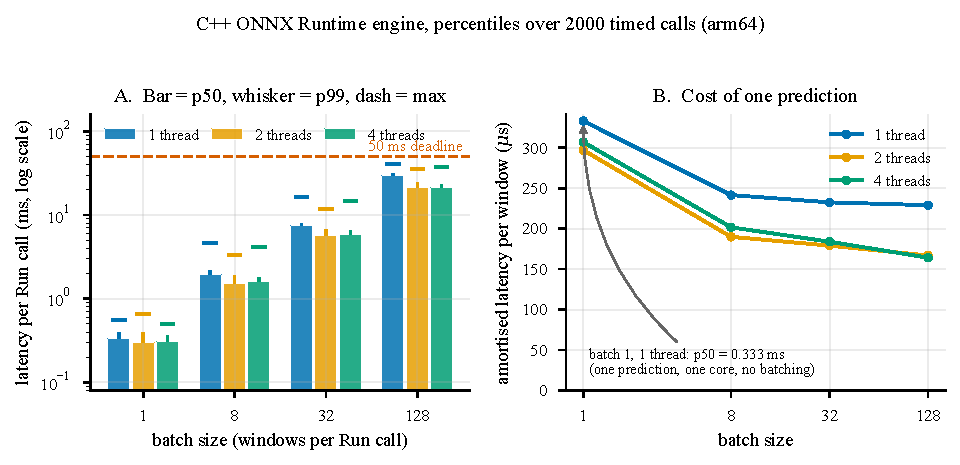
\includegraphics[width=\textwidth]{fig6_edge_latency.pdf}
  \caption{C++ ONNX Runtime engine. (A)~Per-call latency against a
  $\NumEdgeDeadline$~ms deadline; bar is p50, whisker p99, dash the observed
  maximum. (B)~Amortised cost of a single prediction. Percentiles are as
  reported by the runner over its own timed calls.}
  \label{fig:edge}
\end{figure*}

\paragraph{What this section does and does not establish.} We state the scope
first to prevent a likely misreading. These measurements were taken on an \NumEdgeCPU{} ($\NumEdgeCores$ cores), a
desktop-class processor. They are \emph{not} evidence that CausalCGM-MT meets a
real-time budget on an insulin pump, a Cortex-M microcontroller, or a
phone-tethered wearable, and we make no such claim. What they establish is
narrower: the deployment path we ship (ONNX export, a standalone C++ ONNX Runtime
binary, and a C++ reimplementation of the feature construction) adds negligible
overhead of its own. A future port to target silicon is therefore a question
about that silicon rather than about accumulated inefficiency in the serving
stack.

The graph benchmarked has the architecture of the \NumEdgeGraph{} model reported in
Table~\ref{tab:sota_ph30}: the dual-trunk network with cross-attention and both
horizon heads, not a reduced stand-in. The latency artefact records the graph's
file path and parameter count but not its weights, so these timings concern the
architecture and are not shown to belong to the Table~\ref{tab:sota_ph30}
checkpoint. It runs against ONNX Runtime~1.23.2 in
the Release build, timing the \texttt{Run} call alone; the chip is recorded in
the artefact the numbers are read from rather than named here by hand. A single
window costs $\NumEdgePFifty$~ms at the median and $\NumEdgePNinetyNine$~ms at
p99 on one thread, with a worst observed call of $\NumEdgeMax$~ms. Feature
construction adds $\NumEdgeFeatureUs$~$\mu$s per window, roughly three orders of
magnitude below the inference call. This is the specific overhead result the
section reports: the hand-written C++ feature path that must match the training
pipeline bit for bit costs essentially nothing to run. Batching
amortises to $\NumEdgeBestPerWindowUs$~$\mu$s per window at batch
$\NumEdgeBestBatch$ on $\NumEdgeBestThreads$ threads, and single-shot tail
latency is \emph{worse} under batching, so a device serving one window every
five minutes should stay at batch~1.

We report the tail rather than the mean: a p50 of 2~ms with a p99.9 of 80~ms
misses the deadline on one alarm in a thousand, and a mean would not show that. Against the $\NumEdgeDeadline$~ms deadline set for this study (a reading
arrives every five minutes) the measured maximum leaves a factor of $\NumEdgeHeadroomMax$, but that
multiple is a property of this processor and does not transfer. A Cortex-class
core differs from an \NumEdgeCPU{} in vector width, cache hierarchy and memory
bandwidth simultaneously, and quantisation or a CMSIS-NN style kernel rewrite
would change the arithmetic as well. We do not know the target-hardware latency
and this experiment cannot determine it. What the architecture does offer a port
is a static shape (a fixed $H \times C$ input, no recurrence, and no
data-dependent control flow), so the graph is a candidate for ahead-of-time
scheduling and quantisation rather than something that would have to be
redesigned first. Measuring it is future work, and until it is measured the
on-device claim in this paper is about the software stack, not the silicon.

\subsection{Clinical Error Grid Definitions}
\label{sec:appendix_grids}

The Clarke error grid~\citep{clarke1987evaluating} is implemented from the
published rules and validated against canonical points, so the zone boundaries
are ours to audit rather than a library's to assume. The Parkes consensus
grid~\citep{parkes2000new} is delegated to a maintained package and verified
before use. Both partition the reference-against-prediction plane into zones by
the clinical consequence of the error rather than its magnitude, which is why
they are reported alongside RMSE: a 30~mg/dL error at a hypoglycemic reference
and the same error at 250~mg/dL are one number in RMSE and different zones here.
Zone~D is the case a forewarning system exists to avoid, in which the reference
is hypoglycemic, the prediction is normal, and no warning fires.

\subsection{Baseline Configuration Notes}
\label{sec:appendix_baselines}

\paragraph{Why ARIMA's moving-average order is zero.}
\textbf{ARIMA($4,1,0$)}~\citep{box2015time} is fitted per subject by
conditional maximum likelihood on that subject's own training series and applied
causally per window. We fix the moving-average order at zero deliberately: an MA
term is a function of the innovation history, recoverable only by filtering from
the series start, so applying it to a 24-sample window would either require the
full series, which reaches across the official boundary, or start from zero
innovations. With $q = 0$ the $h$-step forecast is a closed-form function of
the window's own lags, which is the only formulation well defined under this
protocol.

% Appendix B -- the 60-minute master benchmark and the controls that say what
% the classical baselines' forewarning columns actually measure.
\section{Extended Benchmark Results (\texorpdfstring{$\PH = 60$}{PH = 60}) and Baseline Controls}
\label{app:benchmarks}

\paragraph*{How to read the classification columns of Tables~\ref{tab:sota_ph30}
and~\ref{tab:sota_ph60}.} Persistence, Ridge-AR and ARIMA have no classification
head. Their PR-AUC, Se@FPR and FAPD entries come from
$\sigma((70 - \hat{y})/\tau)$ applied to a forecast of $g(t{+}\mathrm{PH})$,
while the label is $\min g$ over $(t, t{+}\mathrm{PH}]$. Those three entries are
therefore lower bounds on what the method achieves when fitted to the labelled
quantity, and Table~\ref{tab:ablation_f_nadir_target_ph30} refits Ridge-AR to the
nadir to quantify the gap. LightGBM and both neural arms fit a classifier on the
nadir label directly and are unaffected. This caveat applies to every benchmark
table in the paper; the captions state it in one clause and point here.

\subsection{Sixty-Minute Horizon: Master Benchmark}
\label{sec:appendix_benchmarks}

% These two generated tables have sixteen columns. Set as ordinary table*
% floats they are shrunk to about 5 pt; set landscape (rotating's
% sidewaystable*, inside a group so no other float changes) they print near
% their natural size. The generated files are not edited.
\begingroup
\renewenvironment{table*}[1][]{\begin{sidewaystable*}[p]}{\end{sidewaystable*}}
\begin{table*}[t]
\centering
\small
\setlength{\tabcolsep}{4pt}
\caption{OhioT1DM official test split, PH = 30 min (12 subjects, $n = 28335$ windows). Coverage and width are split-conformal at $\alpha = 0.1$, calibrated on the disjoint calibration split; hypo coverage is the Mondrian $<70$ mg/dL stratum. Persistence, Ridge-AR and ARIMA have no classification head, so their PR-AUC, Se@FPR and FAPD entries are \emph{lower bounds} (Appendix~\ref{app:benchmarks}).}
\label{tab:sota_ph30}
\resizebox{\ifdim\width>\linewidth\linewidth\else\width\fi}{!}{%
\begin{tabular}{lrrrrrrrrrrrrrrr}
\toprule
Model & RMSE & MAE & MARD (\%) & Lag (min) & A+B (\%) & D+E ($n$) & Parkes A+B (\%) & PR-AUC & Se@5\% & Se@10\% & FAPD@5\% & Onset lead (min) & Cov. & Hypo cov. & Width \\
\midrule
Persistence & 23.29 & 16.79 & 11.25 & 30.0 & 99.02 & 272 & 99.66 & 0.832 & 0.933 & 0.970 & 1.16 & 23.7 & 0.913 & \textbf{0.934} & 80.0 \\
Ridge-AR & 20.05 & 14.29 & 9.76 & 25.0 & 98.74 & 351 & 99.76 & 0.829 & 0.964 & 0.990 & 2.99 & 26.4 & 0.916 & 0.933 & 67.7 \\
ARIMA(4,1,0) & 21.09 & 14.89 & 9.94 & 25.0 & 99.31 & 187 & 99.79 & 0.856 & 0.957 & 0.985 & 2.05 & 25.8 & 0.914 & 0.933 & 72.5 \\
LightGBM & \textbf{18.92} & 13.07 & 8.74 & \textbf{20.0} & 99.04 & 270 & 99.81 & 0.841 & \textbf{0.968} & 0.993 & 2.90 & \textbf{27.1} & 0.920 & 0.922 & 66.6 \\
Dilated LSTM (CGM) & 19.52 & 13.39 & 8.80 & 20.0 & \textbf{99.38} & \textbf{175} & \textbf{99.86} & 0.858 & 0.962 & \textbf{0.994} & 2.88 & 26.2 & 0.918 & 0.933 & 68.5 \\
CausalCGM-MT (CGM) & 19.16 & 13.33 & 8.89 & 20.0 & 99.18 & 231 & 99.79 & 0.868 & 0.954 & 0.990 & 2.57 & 25.6 & 0.922 & 0.926 & 68.7 \\
CausalCGM-MT (fusion) & 18.97 & \textbf{13.01} & \textbf{8.52} & 20.0 & 99.34 & 184 & 99.84 & \textbf{0.870} & 0.957 & 0.991 & 2.80 & 26.5 & 0.926 & 0.887 & 68.8 \\
CausalCGM-MT + LoRA ($r = 4$) & 21.81 & 15.82 & 10.52 & 25.0 & 98.86 & 323 & 99.67 & 0.649 & 0.783 & 0.898 & 1.80 & 21.9 & 0.921 & 0.907 & 78.3 \\
\bottomrule
\end{tabular}}
\end{table*}

\begin{table*}[t]
\centering
\small
\setlength{\tabcolsep}{4pt}
\caption{OhioT1DM official test split, PH = 60 min (12 subjects, $n = 28335$ windows). Coverage and width are split-conformal at $\alpha = 0.1$, calibrated on the disjoint calibration split; hypo coverage is the Mondrian $<70$ mg/dL stratum. Persistence, Ridge-AR and ARIMA have no classification head, so their PR-AUC, Se@FPR and FAPD entries are \emph{lower bounds} (Appendix~\ref{app:benchmarks}).}
\label{tab:sota_ph60}
\resizebox{\ifdim\width>\linewidth\linewidth\else\width\fi}{!}{%
\begin{tabular}{lrrrrrrrrrrrrrrr}
\toprule
Model & RMSE & MAE & MARD (\%) & Lag (min) & A+B (\%) & D+E ($n$) & Parkes A+B (\%) & PR-AUC & Se@5\% & Se@10\% & FAPD@5\% & Onset lead (min) & Cov. & Hypo cov. & Width \\
\midrule
Persistence & 38.16 & 28.12 & 19.03 & 60.0 & 96.88 & 700 & 97.84 & 0.724 & 0.789 & 0.866 & 1.25 & 35.8 & 0.909 & 0.928 & 129.9 \\
Ridge-AR & 33.82 & 25.32 & 17.63 & 50.0 & 96.27 & 987 & 98.01 & 0.702 & 0.864 & 0.920 & 3.72 & 45.1 & 0.905 & 0.936 & 112.3 \\
ARIMA(4,1,0) & 36.55 & 26.68 & 17.95 & 55.0 & 97.25 & \textbf{611} & 98.18 & 0.752 & 0.830 & 0.901 & 2.34 & 40.8 & 0.911 & 0.931 & 125.6 \\
LightGBM & 32.12 & 23.13 & 15.53 & 45.0 & 96.93 & 820 & 98.50 & 0.755 & \textbf{0.867} & 0.926 & 3.76 & \textbf{46.0} & 0.910 & 0.939 & 110.5 \\
Dilated LSTM (CGM) & 33.50 & 23.89 & 15.54 & 45.0 & 97.50 & 662 & \textbf{98.81} & 0.766 & 0.858 & 0.920 & 3.28 & 44.5 & 0.911 & \textbf{0.952} & 117.2 \\
CausalCGM-MT (CGM) & 33.07 & 23.70 & 15.80 & 45.0 & 97.21 & 711 & 98.64 & 0.775 & 0.844 & 0.910 & 2.99 & 42.1 & 0.918 & 0.942 & 118.5 \\
CausalCGM-MT (fusion) & \textbf{31.76} & \textbf{22.64} & \textbf{14.83} & \textbf{40.0} & \textbf{97.55} & 676 & 98.78 & \textbf{0.783} & 0.858 & \textbf{0.928} & 3.00 & 44.7 & 0.925 & 0.947 & 117.4 \\
CausalCGM-MT + LoRA ($r = 4$) & 37.59 & 28.01 & 18.72 & 45.0 & 96.96 & 824 & 97.67 & 0.548 & 0.589 & 0.731 & 1.63 & 32.9 & 0.927 & 0.938 & 137.4 \\
\bottomrule
\end{tabular}}
\end{table*}

\endgroup

Tables~\ref{tab:sota_ph30} and~\ref{tab:sota_ph60} give every metric for one
seed ($1337$) at $\PH = 30$ and $60$~min on the official test split. They exist
for completeness: a bold entry marks the best value in that single run and is
not evidence of a difference. Comparisons between arms should be read from the
multi-seed tables below. Persistence, Ridge-AR and ARIMA have no classification
head, so their forewarning columns are lower bounds, which
Appendix~\ref{sec:ablation_f} quantifies.

% A full-page rotated float otherwise waits at the head of the two-column
% float queue and holds every later table back to the end of the paper; flush
% the two landscape tables here, before the next subsection.
\clearpage
\subsection{Multi-Seed Results and Bootstrap Intervals}
\label{sec:appendix_multiseed}

\begin{table*}[t]
\centering
\small
\setlength{\tabcolsep}{4pt}
\caption{Fusion minus each arm at $\PH = 30$~min, seed-mean difference with a 95\% subject-cluster bootstrap CI (12 subjects resampled, 1000 draws). A CI spanning 0 is not a resolved difference.}
\label{tab:multiseed_diffs_ph30}
\resizebox{\ifdim\width>\linewidth\linewidth\else\width\fi}{!}{%
\begin{tabular}{lrrrrr}
\toprule
vs.\ arm & $\Delta$RMSE & $\Delta$PR-AUC & $\Delta$PR-AUC (onset) & $\Delta$FAPD & $\Delta$(D+E) \\
\midrule
Persistence & -4.53 [-5.36, -3.70] & +0.032 [-0.008, +0.069] & +0.104 [-0.006, +0.203] & +1.31 [+0.90, +1.73] & -75 [-123, -28] \\
Ridge-AR & -1.29 [-1.62, -0.88] & +0.034 [+0.014, +0.063] & +0.021 [-0.036, +0.082] & -0.52 [-0.99, -0.08] & -154 [-229, -80] \\
ARIMA(4,1,0) & -2.33 [-2.67, -1.95] & +0.008 [-0.022, +0.041] & +0.032 [-0.062, +0.133] & +0.42 [+0.12, +0.73] & +10 [-27, +47] \\
LightGBM & -0.15 [-0.48, +0.14] & +0.022 [-0.012, +0.053] & -0.023 [-0.098, +0.052] & -0.43 [-0.88, -0.15] & -73 [-125, -24] \\
Dilated LSTM (CGM) & -0.59 [-0.96, -0.24] & +0.000 [-0.019, +0.014] & +0.002 [-0.061, +0.053] & -0.14 [-0.53, +0.11] & +24 [-3, +59] \\
CausalCGM-MT (CGM) & -0.52 [-0.82, -0.23] & +0.001 [-0.013, +0.009] & +0.023 [-0.017, +0.052] & -0.17 [-0.54, +0.14] & +2 [-21, +30] \\
CausalCGM-MT + LoRA (r=4) & -2.85 [-3.51, -2.34] & +0.193 [+0.136, +0.224] & +0.190 [+0.128, +0.235] & +0.69 [-0.11, +1.45] & -145 [-225, -69] \\
\bottomrule
\end{tabular}}
\end{table*}

\begin{table*}[t]
\centering
\small
\setlength{\tabcolsep}{4pt}
\caption{OhioT1DM test split, $\PH = 60$~min: mean $\pm$ sd over 5 training seeds. Alarm thresholds are fitted on the calibration split and applied unchanged to test. PR-AUC (onset) excludes anchors that are below 70~mg/dL now or in the preceding 30~min. Onset lead is minutes from the first valid alert to the first reading below 70. FAPD@5\% counts false alarm episodes under the default alarm policy: an episode lasts while the score stays above threshold, with no merging across gaps and a minimum duration of one reading (5~min); Appendix~\ref{sec:appendix_latching} varies both. Classical arms and LightGBM are deterministic (sd 0).}
\label{tab:sota_multiseed_ph60}
\resizebox{\ifdim\width>\linewidth\linewidth\else\width\fi}{!}{%
\begin{tabular}{lrrrrrrr}
\toprule
Arm & RMSE & PR-AUC & PR-AUC (onset) & Se@5\% (cal.) & FAPD@5\% & Onset lead & D+E \\
\midrule
Persistence & 38.16 $\pm$ 0.00 & 0.724 $\pm$ 0.000 & 0.312 $\pm$ 0.000 & 0.789 $\pm$ 0.000 & 1.25 $\pm$ 0.00 & 35.8 $\pm$ 0.0 & 700 $\pm$ 0 \\
Ridge-AR & 33.82 $\pm$ 0.00 & 0.702 $\pm$ 0.000 & 0.377 $\pm$ 0.000 & 0.864 $\pm$ 0.000 & 3.72 $\pm$ 0.00 & 45.1 $\pm$ 0.0 & 987 $\pm$ 0 \\
ARIMA(4,1,0) & 36.55 $\pm$ 0.00 & 0.752 $\pm$ 0.000 & 0.364 $\pm$ 0.000 & 0.830 $\pm$ 0.000 & 2.34 $\pm$ 0.00 & 40.8 $\pm$ 0.0 & 611 $\pm$ 0 \\
LightGBM & 32.12 $\pm$ 0.00 & 0.755 $\pm$ 0.000 & 0.431 $\pm$ 0.000 & 0.867 $\pm$ 0.000 & 3.76 $\pm$ 0.00 & 46.0 $\pm$ 0.0 & 820 $\pm$ 0 \\
Dilated LSTM (CGM) & 33.30 $\pm$ 0.31 & 0.773 $\pm$ 0.009 & 0.408 $\pm$ 0.022 & 0.859 $\pm$ 0.001 & 3.24 $\pm$ 0.27 & 44.7 $\pm$ 0.7 & 643 $\pm$ 21 \\
CausalCGM-MT (CGM) & 33.32 $\pm$ 0.23 & 0.774 $\pm$ 0.003 & 0.401 $\pm$ 0.016 & 0.846 $\pm$ 0.013 & 3.10 $\pm$ 0.14 & 43.1 $\pm$ 1.3 & 690 $\pm$ 49 \\
CausalCGM-MT (fusion) & 31.85 $\pm$ 0.37 & 0.774 $\pm$ 0.009 & 0.413 $\pm$ 0.022 & 0.847 $\pm$ 0.009 & 2.84 $\pm$ 0.32 & 43.9 $\pm$ 0.7 & 617 $\pm$ 53 \\
CausalCGM-MT + LoRA (r=4) & 37.62 $\pm$ 0.95 & 0.564 $\pm$ 0.065 & 0.237 $\pm$ 0.035 & 0.622 $\pm$ 0.069 & 1.78 $\pm$ 0.21 & 34.1 $\pm$ 1.8 & 859 $\pm$ 31 \\
\bottomrule
\end{tabular}}
\end{table*}

\begin{table*}[t]
\centering
\small
\setlength{\tabcolsep}{4pt}
\caption{Fusion minus each arm at $\PH = 60$~min, seed-mean difference with a 95\% subject-cluster bootstrap CI (12 subjects resampled, 1000 draws). A CI spanning 0 is not a resolved difference.}
\label{tab:multiseed_diffs_ph60}
\resizebox{\ifdim\width>\linewidth\linewidth\else\width\fi}{!}{%
\begin{tabular}{lrrrrr}
\toprule
vs.\ arm & $\Delta$RMSE & $\Delta$PR-AUC & $\Delta$PR-AUC (onset) & $\Delta$FAPD & $\Delta$(D+E) \\
\midrule
Persistence & -6.31 [-7.77, -5.04] & +0.050 [-0.003, +0.095] & +0.101 [-0.014, +0.200] & +1.59 [+1.10, +2.06] & -83 [-171, +11] \\
Ridge-AR & -1.97 [-2.92, -1.01] & +0.071 [+0.036, +0.110] & +0.036 [-0.024, +0.099] & -0.88 [-1.61, -0.33] & -370 [-649, -170] \\
ARIMA(4,1,0) & -4.70 [-5.78, -3.66] & +0.022 [-0.020, +0.063] & +0.049 [-0.041, +0.139] & +0.51 [+0.01, +0.91] & +6 [-66, +98] \\
LightGBM & -0.27 [-1.00, +0.50] & +0.018 [-0.015, +0.047] & -0.019 [-0.080, +0.040] & -0.92 [-1.66, -0.40] & -203 [-315, -106] \\
Dilated LSTM (CGM) & -1.45 [-2.32, -0.59] & +0.000 [-0.022, +0.016] & +0.004 [-0.035, +0.032] & -0.40 [-0.91, -0.01] & -26 [-73, +31] \\
CausalCGM-MT (CGM) & -1.47 [-2.20, -0.77] & +0.000 [-0.023, +0.016] & +0.012 [-0.040, +0.047] & -0.25 [-0.71, +0.15] & -73 [-120, -23] \\
CausalCGM-MT + LoRA (r=4) & -5.77 [-7.14, -4.57] & +0.210 [+0.142, +0.268] & +0.175 [+0.132, +0.220] & +1.06 [+0.18, +2.01] & -242 [-375, -129] \\
\bottomrule
\end{tabular}}
\end{table*}


Table~\ref{tab:sota_multiseed_ph30} (main text) and
Table~\ref{tab:sota_multiseed_ph60} report means over $\NumMSSeeds$ seeds;
classical arms and LightGBM are deterministic. CIs resample the twelve subjects,
so they reflect between-subject variation, and twelve clusters make them
approximate. Three readings follow. Fusion improves RMSE over the CGM-only
network at both horizons, with CIs excluding zero. Fusion and LightGBM are not
separated on RMSE or PR-AUC at either horizon. The three neural arms are not
separated on PR-AUC, so no arm leads on forewarning.

\subsection{Sensitivity of False-Alarm Burden to the Alarm Policy}
\label{sec:appendix_latching}

\begin{table*}[t]
\centering
\small
\setlength{\tabcolsep}{4pt}
\caption{False alarms per day / onset detection rate at $\PH = 30$~min under alternative alarm policies, mean over 5 seeds. G: latching gap (min) within which a new above-threshold run does not sound again; D: minimum duration (min) before an alarm sounds. G=0, D=5 is the policy used elsewhere in the paper. Thresholds are each seed's calibration-split 5\%-FPR thresholds, not refitted per policy.}
\label{tab:fapd_latching}
\resizebox{\ifdim\width>\linewidth\linewidth\else\width\fi}{!}{%
\begin{tabular}{lrrrrrrr}
\toprule
Policy (G, D) & Persist. & Ridge & ARIMA & LGBM & LSTM & TCN-CGM & Fusion \\
\midrule
G=0, D=5 & 1.16 / 95\% & 2.99 / 95\% & 2.05 / 95\% & 2.90 / 95\% & 2.61 / 95\% & 2.64 / 95\% & 2.47 / 94\% \\
G=5, D=5 & 1.06 / 95\% & 2.22 / 95\% & 1.76 / 95\% & 2.44 / 95\% & 2.01 / 95\% & 1.90 / 95\% & 1.85 / 94\% \\
G=15, D=5 & 1.01 / 95\% & 1.69 / 95\% & 1.47 / 95\% & 1.99 / 95\% & 1.63 / 95\% & 1.55 / 95\% & 1.52 / 94\% \\
G=30, D=5 & 0.90 / 95\% & 1.51 / 95\% & 1.29 / 95\% & 1.63 / 95\% & 1.38 / 95\% & 1.27 / 95\% & 1.33 / 94\% \\
G=60, D=5 & 0.80 / 95\% & 1.32 / 95\% & 1.15 / 95\% & 1.38 / 95\% & 1.12 / 95\% & 1.11 / 95\% & 1.10 / 94\% \\
G=0, D=10 & 1.07 / 90\% & 1.73 / 93\% & 1.50 / 94\% & 1.70 / 94\% & 1.60 / 93\% & 1.53 / 93\% & 1.58 / 91\% \\
G=0, D=15 & 0.89 / 84\% & 1.13 / 93\% & 1.07 / 89\% & 1.13 / 90\% & 1.20 / 90\% & 1.09 / 90\% & 1.09 / 87\% \\
\bottomrule
\end{tabular}}
\end{table*}


FAPD counts alarm episodes, so it depends on what ends an episode. The default
policy ends an alarm as soon as the score dips below threshold, so a single
5-minute dip produces a second sounding. Table~\ref{tab:fapd_latching} re-scores
every arm under two alternatives, holding each seed's calibration-fitted
threshold fixed: latching across gaps of up to $G$ minutes, and a minimum
duration of $D$ minutes before an alarm sounds. Absolute FAPD is highly
policy-dependent: fusion falls from $\NumLatchBaseFusionFAPD$ to
$\NumLatchGSixtyFusionFAPD$ false alarms per day under 60-minute latching, so
FAPD values are comparable only within a policy. Persistence has the lowest FAPD
under every policy tested, at the cost of the shortest onset lead. Fusion's lower
FAPD than LightGBM under latching does not come free: under a 15-minute minimum
duration, fusion detects $\NumLatchDFifteenFusionDet\%$ of onsets against
LightGBM's $\NumLatchDFifteenLGBMDet\%$ (difference $\NumLatchDFifteenDetDiffLGBM$
points, 95\% subject-bootstrap CI $[\NumLatchDFifteenDetDiffLGBMLo,
\NumLatchDFifteenDetDiffLGBMHi]$).

\subsection{Ablation F: Is the Endpoint Baseline Handicapped?}
\label{sec:ablation_f}

\begin{table*}[t]
\centering
\small
\setlength{\tabcolsep}{4pt}
\caption{Ablation F: is the endpoint baseline handicapped by its risk mapping? (PH = 30 min). Classification metrics only. Persistence, Ridge-AR and ARIMA have no classification head and score hypoglycemia through $\sigma((70 - \hat{y})/\tau)$, a strictly monotone map of their forecast; the label is the window \emph{minimum}, which an endpoint forecast does not target. The nadir arms are the identical Ridge-AR fitted to $\min g$ over $(t, t+\mathrm{PH}]$ instead of $g(t+\mathrm{PH})$ and mapped the same way, so the difference between the two rows is the target alone. LightGBM and every neural arm fit a classifier on the nadir label directly and are shown for reference, not as part of the contrast. All ablation arms share one budget (20 epochs, fit split subsampled $2\times$), lighter than Table~\ref{tab:sota_ph30}'s (30 epochs, full fit split); rows here compare to each other, not to Table~\ref{tab:sota_ph30}.}
\label{tab:ablation_f_nadir_target_ph30}
\resizebox{\ifdim\width>\linewidth\linewidth\else\width\fi}{!}{%
\begin{tabular}{lrrrrr}
\toprule
Arm & PR-AUC & ROC-AUC & Se@5\% & FAPD@5\% & Onset lead (min) \\
\midrule
Ridge-AR, level target & 0.829 & 0.9900 & 0.964 & 2.99 & 26.4 \\
Ridge-AR, nadir target & 0.861 & 0.9900 & 0.962 & 2.25 & 26.0 \\
LightGBM (native nadir classifier) & 0.841 & \textbf{0.9916} & \textbf{0.968} & 2.90 & \textbf{27.1} \\
CausalCGM-MT (native nadir head) & \textbf{0.865} & 0.9912 & 0.959 & 2.87 & 26.4 \\
\bottomrule
\end{tabular}}
\end{table*}

\begin{table*}[t]
\centering
\small
\setlength{\tabcolsep}{4pt}
\caption{Ablation F: is the endpoint baseline handicapped by its risk mapping? (PH = 60 min). Classification metrics only. Persistence, Ridge-AR and ARIMA have no classification head and score hypoglycemia through $\sigma((70 - \hat{y})/\tau)$, a strictly monotone map of their forecast; the label is the window \emph{minimum}, which an endpoint forecast does not target. The nadir arms are the identical Ridge-AR fitted to $\min g$ over $(t, t+\mathrm{PH}]$ instead of $g(t+\mathrm{PH})$ and mapped the same way, so the difference between the two rows is the target alone. LightGBM and every neural arm fit a classifier on the nadir label directly and are shown for reference, not as part of the contrast. All ablation arms share one budget (20 epochs, fit split subsampled $2\times$), lighter than Table~\ref{tab:sota_ph30}'s (30 epochs, full fit split); rows here compare to each other, not to Table~\ref{tab:sota_ph30}.}
\label{tab:ablation_f_nadir_target_ph60}
\resizebox{\ifdim\width>\linewidth\linewidth\else\width\fi}{!}{%
\begin{tabular}{lrrrrr}
\toprule
Arm & PR-AUC & ROC-AUC & Se@5\% & FAPD@5\% & Onset lead (min) \\
\midrule
Ridge-AR, level target & 0.702 & 0.9650 & 0.864 & 3.72 & 45.1 \\
Ridge-AR, nadir target & 0.757 & 0.9640 & 0.840 & 2.68 & 42.0 \\
LightGBM (native nadir classifier) & 0.755 & \textbf{0.9718} & \textbf{0.867} & 3.76 & \textbf{46.0} \\
CausalCGM-MT (native nadir head) & \textbf{0.772} & 0.9714 & 0.849 & 3.37 & 43.5 \\
\bottomrule
\end{tabular}}
\end{table*}


Section~\ref{sec:baselines} flagged an asymmetry in the benchmark table:
persistence, Ridge-AR and ARIMA are scored on a nadir label through a monotone
map of an endpoint forecast. This study measures what that costs them, by
refitting Ridge-AR to $\min g$ over $(t, t{+}\PH]$ instead of $g(t{+}\PH)$. The
design matrix, the ridge penalty, the residual parameterisation and the risk
mapping are all unchanged; only the regression target moves, so the difference
between the two rows is attributable to the target and nothing else.

\textbf{The handicap is real and we were understating these baselines.}
Targeting the nadir raises Ridge-AR's PR-AUC by $\NumAblFNadirGainHThirty$ at
$\PH = 30$ and $\NumAblFNadirGainHSixty$ at $\PH = 60$, and lowers its
false-alarm rate from $\NumAblFRidgeLevelFAPDHThirty$ to
$\NumAblFRidgeNadirFAPDHThirty$ per day. ROC-AUC barely moves
($\NumAblFRidgeLevelROCAUCHThirty \to \NumAblFRidgeNadirROCAUCHThirty$), which
locates the gain precisely: the endpoint forecast ranks the bulk of the
distribution just as well, and what it was losing was precision on the rare
positive class. More specifically, those are the transient nadirs that recover
before the horizon, which are the events the label is built around and the
endpoint cannot see. At
$\PH = 30$ the nadir-targeted Ridge-AR ($\NumAblFRidgeNadirPRAUCHThirty$) also
overtakes LightGBM's native classifier ($\NumAblFLGBMPRAUCHThirty$), so this is
not a small correction to an also-ran.

\textbf{With the baseline corrected, the network's forewarning advantage is
not established.} Against nadir-targeted Ridge-AR, CausalCGM-MT is ahead by
$\NumAblFMTLeadOverNadirHThirty$ PR-AUC at $\PH = 30$ and
$\NumAblFMTLeadOverNadirHSixty$ at $\PH = 60$ in this single-seed study. Those
gaps are compared here with the seed-to-seed standard deviation of each neural
arm's PR-AUC in the multi-seed tables. At $\PH = 30$ these are
$\NumMSFusionPRAUCHThirtySD$ (fusion), $\NumMSLSTMPRAUCHThirtySD$ (LSTM) and
$\NumMSCGMOnlyPRAUCHThirtySD$ (CGM-only); at $\PH = 60$ they are
$\NumMSFusionPRAUCHSixtySD$, $\NumMSLSTMPRAUCHSixtySD$ and
$\NumMSCGMOnlyPRAUCHSixtySD$. The $\PH = 30$ gap is below all three. The
$\PH = 60$ gap is under two standard deviations of the fusion and LSTM arms
but several times that of the CGM-only arm, and it comes from one seed, so we
do not claim a lead over a well-posed classical baseline. A claim
that rests on a baseline being asked the wrong question is not a claim about the
model.

It follows that the classification columns for persistence, Ridge-AR and ARIMA
in the benchmark tables are lower bounds on what those methods achieve when
targeted at the labelled quantity, and should not be cited as the ceiling for
classical forecasting.

\subsection{What the Sigmoid Mapping Measures}
\label{sec:appendix_sigmoid}

The mapping asks those three arms an uneven question. The label is $\min g$ over
$(t, t{+}\PH]$; a level forecast at $t{+}\PH$ is blind to a nadir at $t{+}20$
that recovers by $t{+}30$, and no monotone map of that forecast can recover what
the forecast did not encode. Their classification columns therefore measure two
things at once: how well the arm forecasts, and how much nadir information a
$t{+}\PH$ endpoint carries. Section~\ref{sec:ablation_f} separates them by
fitting the same arm to the nadir directly.

% Appendix C -- the full ablation suite. Ablations B and D keep their PH = 30
% tables in the body; their 60-minute halves and extended discussion are here.
\section{Comprehensive Ablation Studies}
\label{app:ablations}

\subsection{Ablation A: Does Multi-Task Coupling Help?}
\label{sec:ablation_a}

\begin{table*}[t]
\centering
\small
\setlength{\tabcolsep}{4pt}
\caption{Ablation A: multi-task coupling (PH = 30 min). Single-task arms zero the other task's loss weight, so the trunk is trained by one objective; the untrained head's metrics are reported but not meaningful. All ablation arms share one budget (20 epochs, fit split subsampled $2\times$), lighter than Table~\ref{tab:sota_ph30}'s (30 epochs, full fit split); rows here compare to each other, not to Table~\ref{tab:sota_ph30}.}
\label{tab:ablation_a_multitask_ph30}
\resizebox{\ifdim\width>\linewidth\linewidth\else\width\fi}{!}{%
\begin{tabular}{lrrrrrrrr}
\toprule
Arm & PR-AUC & ROC-AUC & Se@5\% & FAPD@5\% & Onset lead (min) & RMSE & Lag (min) & A+B (\%) \\
\midrule
Regression only & 0.028 & 0.3187 & 0.030 & 5.61 & 26.2 & \textbf{18.19} & \textbf{20.0} & 99.34 \\
Classification only & \textbf{0.868} & \textbf{0.9915} & \textbf{0.963} & 2.06 & \textbf{26.4} & 23.27 & 30.0 & 98.96 \\
Joint, fixed $\lambda=1$ & 0.842 & 0.9890 & 0.952 & 2.72 & 26.0 & 18.37 & 20.0 & \textbf{99.39} \\
Joint, Kendall uncertainty & 0.865 & 0.9912 & 0.959 & 2.87 & 26.4 & 18.49 & 20.0 & 99.36 \\
\bottomrule
\end{tabular}}
\end{table*}

\begin{table*}[t]
\centering
\small
\setlength{\tabcolsep}{4pt}
\caption{Ablation A: multi-task coupling (PH = 60 min). Single-task arms zero the other task's loss weight, so the trunk is trained by one objective; the untrained head's metrics are reported but not meaningful. All ablation arms share one budget (20 epochs, fit split subsampled $2\times$), lighter than Table~\ref{tab:sota_ph30}'s (30 epochs, full fit split); rows here compare to each other, not to Table~\ref{tab:sota_ph30}.}
\label{tab:ablation_a_multitask_ph60}
\resizebox{\ifdim\width>\linewidth\linewidth\else\width\fi}{!}{%
\begin{tabular}{lrrrrrrrr}
\toprule
Arm & PR-AUC & ROC-AUC & Se@5\% & FAPD@5\% & Onset lead (min) & RMSE & Lag (min) & A+B (\%) \\
\midrule
Regression only & 0.109 & 0.6749 & 0.143 & 4.77 & 41.2 & \textbf{30.84} & \textbf{40.0} & 97.73 \\
Classification only & \textbf{0.775} & \textbf{0.9728} & \textbf{0.856} & 2.37 & 42.7 & 38.13 & 60.0 & 96.91 \\
Joint, fixed $\lambda=1$ & 0.761 & 0.9703 & 0.840 & 3.29 & 43.5 & 31.29 & 40.0 & \textbf{97.93} \\
Joint, Kendall uncertainty & 0.772 & 0.9714 & 0.849 & 3.37 & \textbf{43.5} & 31.61 & 40.0 & 97.80 \\
\bottomrule
\end{tabular}}
\end{table*}


Single-task arms are obtained by zeroing the other task's loss weight, so the
four arms differ only in the objective; a gradient test confirms the silenced
head receives none, and its reported metrics are consequently meaningless.

Model selection follows each arm's own objective, and we state the monitors
explicitly because leaving them implicit would invite exactly the suspicion the
choice is meant to avoid. The regression-only arm is early-stopped on
\texttt{val/rmse} (minimised); the classification-only arm and both joint arms
are early-stopped on \texttt{val/pr\_auc} (maximised). Patience, maximum epochs,
optimiser, seed and every other budget parameter are identical across the four.
Using one monitor for all of them was the alternative and it is worse in both
directions: early-stopping the regression-only arm on PR-AUC would select on a
head that received no gradient, i.e.\ on noise, while early-stopping the
classification-only arm on RMSE would do the same in reverse. Each arm is
therefore stopped at its own best, which is the comparison that gives the
single-task specialists their strongest showing, which are the arms this study is
designed to be compared against unfavourably. The monitor is recorded in each arm's serialised
specification in the results JSON, so the choice is auditable rather than
asserted.

Joint training costs a little of each specialist. At $\PH = 30$ the
classification-only arm reaches PR-AUC $\NumAblAClsPRAUCHThirty$ and the joint
Kendall model $\NumAblAKendallPRAUCHThirty$, a cost of
$\NumAblAMultitaskCostHThirty$; the regression-only arm reaches RMSE
$\NumAblARegRMSEHThirty$ against the joint model's
$\NumAblAKendallRMSEHThirty$.

The comparison this study was designed to test, Kendall weighting against a fixed
$\lambda = 1$ (not tuned), does not resolve. Kendall weighting has the higher
PR-AUC, by $\NumAblAKendallEdgeHThirty$ at $\PH = 30$ and
$\NumAblAKendallEdgeHSixty$ at $\PH = 60$, and the fixed weight has the lower
RMSE at both horizons. Each is one run, and the differences are comparable to
the seed-to-seed range of the neural arms in the multi-seed benchmark. We therefore make
no accuracy claim for uncertainty weighting.

\paragraph{The case for the joint head is a deployment constraint, not an
accuracy claim.} We want to be explicit about this, because the ablation invites
the opposite reading: the specialists are not beaten, and a reader is right to
ask why the coupled model is preferred when a classification-only arm reaches
$\NumAblAClsPRAUCHThirty$ PR-AUC. The answer is that the target is an embedded
medical device, and on such a device the relevant comparison is not one joint
model against one specialist but one joint model against \emph{two} specialists
that must both be resident. A system that regresses glucose and forewarns
hypoglycemia needs both outputs at every five-minute tick; separating them means
shipping and maintaining two model binaries, two sets of weights in flash, two
inference sessions in a fixed RAM budget, two export-and-parity gates in the
release pipeline, and two artefacts to re-certify whenever either is retrained.
The trunk is where nearly all the parameters and nearly all the arithmetic live,
and the two tasks read the same physiology at the same lead times, so the
duplicated trunk serves no purpose.

Set against that, the measured price of coupling is
$\NumAblAMultitaskCostHThirty$ PR-AUC at $\PH = 30$ and a comparable margin on
RMSE ($\NumAblARegRMSEHThirty$ specialist against
$\NumAblAKendallRMSEHThirty$ joint). One trunk, four heads, one set of weights,
one conformal calibration and one $\NumEdgePFifty$~ms inference call
(Section~\ref{sec:edge}) deliver both outputs and their intervals for that
margin. Uncertainty weighting earns its place inside that design for a
maintenance reason rather than an accuracy one: the two losses live on
incompatible scales, so a fixed $\lambda$ is a hyperparameter that must be
re-tuned whenever the horizon set, the cohort or the class prior changes, and a
device pipeline is exactly where such a knob is most expensive to get wrong. We
present the multi-task head as Pareto-optimal under the deployment constraint,
not as a win on the accuracy axis the ablation measures. Had the coupling cost
been large rather than a few thousandths of PR-AUC, that argument would not have
been available.

\subsection{Ablation B: The Asymmetry Trade-Off}
\label{sec:appendix_ablation_b}

\begin{table*}[t]
\centering
\small
\setlength{\tabcolsep}{4pt}
\caption{Ablation B: asymmetric hypoglycemia cost (PH = 30 min). $\kappa$ multiplies the regression loss when the reference is hypoglycemic and the prediction sits above it; $\kappa = 1$ is a no-op. All ablation arms share one budget (20 epochs, fit split subsampled $2\times$), lighter than Table~\ref{tab:sota_ph30}'s (30 epochs, full fit split); rows here compare to each other, not to Table~\ref{tab:sota_ph30}.}
\label{tab:ablation_b_asymmetry_ph30}
\resizebox{\ifdim\width>\linewidth\linewidth\else\width\fi}{!}{%
\begin{tabular}{lrrrrrrr}
\toprule
Arm & RMSE & RMSE $<$70 & Bias $<$70 & D+E ($n$) & A+B (\%) & PR-AUC & Se@5\% \\
\midrule
$\kappa$ = 1 & \textbf{18.24} & 15.28 & +9.98 & 258 & 99.08 & \textbf{0.868} & \textbf{0.959} \\
$\kappa$ = 2 & 18.35 & 13.98 & +7.83 & 211 & 99.24 & 0.863 & 0.958 \\
$\kappa$ = 3 & 18.49 & 12.97 & +6.70 & 179 & 99.36 & 0.865 & 0.959 \\
$\kappa$ = 5 & 18.67 & 11.63 & +4.45 & 147 & 99.47 & 0.855 & 0.946 \\
$\kappa$ = 8 & 18.90 & \textbf{11.06} & +3.07 & \textbf{119} & \textbf{99.57} & 0.856 & 0.946 \\
\bottomrule
\end{tabular}}
\end{table*}

\begin{table*}[t]
\centering
\small
\setlength{\tabcolsep}{4pt}
\caption{Ablation B: asymmetric hypoglycemia cost (PH = 60 min). $\kappa$ multiplies the regression loss when the reference is hypoglycemic and the prediction sits above it; $\kappa = 1$ is a no-op. All ablation arms share one budget (20 epochs, fit split subsampled $2\times$), lighter than Table~\ref{tab:sota_ph30}'s (30 epochs, full fit split); rows here compare to each other, not to Table~\ref{tab:sota_ph30}.}
\label{tab:ablation_b_asymmetry_ph60}
\resizebox{\ifdim\width>\linewidth\linewidth\else\width\fi}{!}{%
\begin{tabular}{lrrrrrrr}
\toprule
Arm & RMSE & RMSE $<$70 & Bias $<$70 & D+E ($n$) & A+B (\%) & PR-AUC & Se@5\% \\
\midrule
$\kappa$ = 1 & \textbf{30.92} & 29.72 & +22.78 & 701 & 97.41 & \textbf{0.777} & \textbf{0.862} \\
$\kappa$ = 2 & 31.29 & 30.06 & +21.33 & 630 & 97.65 & 0.772 & 0.854 \\
$\kappa$ = 3 & 31.61 & 27.63 & +18.83 & 583 & 97.80 & 0.772 & 0.849 \\
$\kappa$ = 5 & 32.04 & 24.49 & +14.71 & 496 & 98.15 & 0.757 & 0.826 \\
$\kappa$ = 8 & 32.31 & \textbf{23.88} & +13.23 & \textbf{477} & \textbf{98.20} & 0.760 & 0.839 \\
\bottomrule
\end{tabular}}
\end{table*}


Table~\ref{tab:ablation_b_asymmetry_ph30} shows the $\kappa$ sweep at $\PH = 30$~min, 
and Table~\ref{tab:ablation_b_asymmetry_ph60} repeats it at $\PH = 60$~min. The trade-off has the
same shape at the longer horizon: raising $\kappa$ buys accuracy and signed bias
below 70~mg/dL and pays for it in overall RMSE and forewarning discrimination.
The operating-point argument of Section~\ref{sec:results} is therefore
not specific to the thirty-minute horizon it is made at.

\paragraph{Why the shared trunk makes this one decision.}
The shared trunk is what keeps that judgement a single decision. Because $\kappa$
weights the regression term inside the same objective that trains the forewarning
head, moving along this curve re-tunes both outputs at once and yields one binary
per operating point. Under a two-model deployment the same choice would have to
be made twice, in two loss functions that no longer see each other's
residuals, and the regression model's downward shift below 70~mg/dL would
silently move the input distribution that the separately trained classifier had
been calibrated against. Here it cannot: both heads read the forward pass the
asymmetry shifts, so Figure~\ref{fig:tradeoff} reports the whole exchange rate
rather than one model's half of it.

\paragraph{How finely the $\kappa$ curve should be read.}
At the repository default $\kappa = 3$, bias falls $\NumBiasDropThree\%$ and
zone D+E errors $\NumDEDropThree\%$ for $\NumKappaThreeRMSECostPct\%$ overall
RMSE and $\NumKappaThreePRAUCDrop$ PR-AUC. Two cautions about how finely this
curve should be read. At $\PH = 30$, zone D+E counts, RMSE below 70~mg/dL and
the signed hypoglycemic bias fall monotonically in $\kappa$ while overall RMSE
rises monotonically; these are the reliable part of the trade. PR-AUC is
\emph{not} monotone, and its range across the five arms is comparable to the
seed-to-seed variation of the multi-seed benchmark, so a single run cannot
resolve it. At $\PH = 60$ RMSE below 70~mg/dL is not monotone either. We therefore
claim only the direction (raising $\kappa$ buys dangerous-zone errors and pays in
overall accuracy and discrimination) and not an optimum. A sweep reporting only RMSE and zone
counts would imply a free lunch; one reading a few thousandths of PR-AUC as a
maximum would invent an operating point the data does not support. Which point
on this curve is acceptable is a clinical judgement about the relative cost of a
missed low versus an unnecessary snack, not a modelling one, and the figure is
offered so that judgement can be made with the exchange rate visible (see
Appendix~\ref{sec:appendix_clarke}, Figure~\ref{fig:clarke}, for the
corresponding Clarke grid migrations, and
Appendix~\ref{sec:appendix_ablation_b} for the same sweep at $\PH = 60$~min).

\subsection{Clinical Safety Under the Asymmetry}
\label{sec:appendix_clarke}

\begin{figure*}[t]
  \centering
  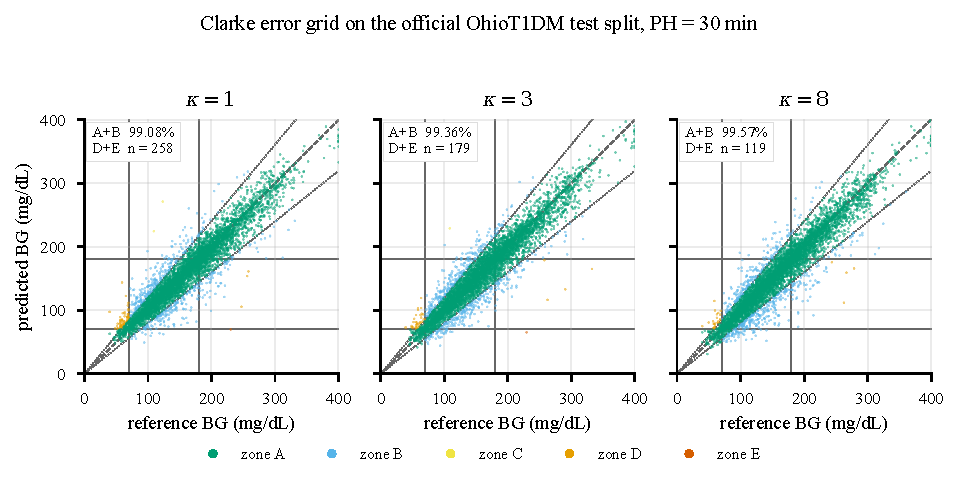
\includegraphics[width=\textwidth]{fig3_clarke_parkes_grids.pdf}
  \caption{Clarke error grid on the official OhioT1DM test split,
  $\PH = 30$~min, at three values of the asymmetry $\kappa$. Points migrate out
  of the dangerous lower-right region as $\kappa$ rises; zone percentages are
  computed on the full test set, not the plotted subsample.}
  \label{fig:clarke}
\end{figure*}

Figure~\ref{fig:clarke} shows the mechanism directly. The dangerous region for a
warning system is the lower-right (reference hypoglycemic, prediction normal),
and raising $\kappa$ empties it at the cost of a slight downward shift
elsewhere.

\subsection{Ablation C: Which Auxiliary Inputs Carry the Fusion Gain?}
\label{sec:ablation_c}

\begin{table*}[t]
\centering
\small
\setlength{\tabcolsep}{4pt}
\caption{Ablation C, condensed: every auxiliary arm as a change from its \emph{own} cohort's CGM-only control, which is the only comparison the design supports -- the 2018 and 2020 releases carry disjoint sensors, so the two blocks are not comparable to each other. Negative $\Delta$RMSE and positive $\Delta$PR-AUC are improvements. Each arm is one seed on six subjects, so the deltas are directions, not resolved effects: treatment inputs lower RMSE in both cohorts and at both horizons, and wearable streams do not do so consistently. Per-cohort tables with every metric are in the artefact directory. All ablation arms share one budget (20 epochs, fit split subsampled $2\times$), lighter than Table~\ref{tab:sota_ph30}'s (30 epochs, full fit split); rows here compare to each other, not to Table~\ref{tab:sota_ph30}.}
\label{tab:ablation_c_modality_summary}
\resizebox{\ifdim\width>\linewidth\linewidth\else\width\fi}{!}{%
\begin{tabular}{lrrrrr}
\toprule
Arm & $\Delta$RMSE 30 & $\Delta$PR-AUC 30 & $\Delta$RMSE 60 & $\Delta$PR-AUC 60 & $n$ subj \\
\midrule
2018: CGM + HR & +0.25 & -0.009 & +0.52 & -0.011 & 6 \\
2018: CGM + GSR & +0.19 & -0.022 & +0.61 & -0.023 & 6 \\
2018: CGM + steps & -0.06 & +0.008 & -0.44 & +0.008 & 6 \\
2018: CGM + treatment & -0.35 & -0.007 & -0.71 & +0.003 & 6 \\
2018: CGM + all auxiliary (incl. treatment) & -0.28 & +0.022 & -0.43 & +0.017 & 6 \\
2020: CGM + accel & -0.02 & -0.012 & +0.10 & +0.000 & 6 \\
2020: CGM + GSR & -0.09 & -0.014 & +0.05 & -0.003 & 6 \\
2020: CGM + treatment & -1.02 & +0.004 & -2.24 & -0.002 & 6 \\
2020: CGM + all auxiliary (incl. treatment) & -0.94 & -0.001 & -2.11 & +0.001 & 6 \\
\bottomrule
\end{tabular}}
\end{table*}


This study asks which auxiliary inputs carry the fusion gain. The two cohorts
wore devices with disjoint sensor sets, so an arm requiring heart rate is
measurable only on the 2018 subjects and one requiring acceleration only on
2020. Each cohort therefore gets its own CGM-only control drawn from the same six
subjects, and we do not rank across cohorts. Every arm is one seed on six
subjects, so individual deltas are directions, not resolved effects.

Wearable streams alone show no consistent benefit. At $\PH = 30$ their effects
are small, are not consistent in sign across cohorts, and
several are unfavourable: heart rate and GSR are worse than the CGM-only control
on 2018 at both horizons. The exception is steps on 2018 at $\PH = 60$, which
lowers RMSE; with one seed on six subjects we read it as a direction to re-test,
not as an effect. Treatment inputs are different. Adding insulin and carbohydrate
channels alone lowers RMSE in both cohorts and at both horizons
($\NumAblCTreatTwentyRMSEHThirty$ and $\NumAblCTreatEighteenRMSEHThirty$~mg/dL at
30~min; $\NumAblCTreatTwentyRMSEHSixty$ and $\NumAblCTreatEighteenRMSEHSixty$ at
60~min), and on RMSE the arm with every auxiliary channel, which includes them, does no
better than treatment alone. The multi-seed fusion gain of
Section~\ref{sec:results} is therefore attributable to treatment inputs. The
per-cohort tables carrying every metric are released with the artefacts.

The fusion trunk adds a \emph{gated residual} to the CGM path
(Equation~\ref{eq:fusion}), so with no auxiliary data the fusion term is exactly
zero. A unit test asserts that the multimodal forward pass reproduces the
CGM-only pass \emph{exactly} when the auxiliary channels are masked. That test is
what caught two defects that left every accuracy metric plausible: a
normalisation placed on the summed representation, and auxiliary validity read
from a single sensor's mask. A third defect of the same kind survived it and was
found only after submission: the per-window presence flag ignored treatment
channels, which have no observation mask, so insulin and carbohydrate inputs
could not enable the fusion branch (Appendix~\ref{sec:metabonet}). The results
here are from the corrected code.

The identity above is architectural, not a performance bound: the CGM path is
trained jointly with the fusion path, and several wearable arms land below their
control at the point estimate.

\subsection{Leakage Ladder at Sixty Minutes}
\label{sec:appendix_ablation_d}

\begin{table*}[t]
\centering
\small
\setlength{\tabcolsep}{4pt}
\caption{Ablation D: what lookahead bias buys (PH = 60 min). Arms are \emph{not} scored on the same test set: changing the split is the flaw being measured. All ablation arms share one budget (20 epochs, fit split subsampled $2\times$), lighter than Table~\ref{tab:sota_ph30}'s (30 epochs, full fit split); rows here compare to each other, not to Table~\ref{tab:sota_ph30}.}
\label{tab:ablation_d_leakage_ph60}
\resizebox{\ifdim\width>\linewidth\linewidth\else\width\fi}{!}{%
\begin{tabular}{lrrrrrrr}
\toprule
Arm & RMSE & MAE & PR-AUC & Se@5\% & A+B (\%) & Lag (min) & $n$ test \\
\midrule
Strict causal pipeline (ours) & 31.61 & 22.63 & 0.772 & 0.849 & 97.80 & 40.0 & 28335 \\
+ unembargoed random split & 30.07 & 21.34 & 0.811 & 0.846 & 98.01 & -- & 29932 \\
+ full-series interpolation \& centred features & 27.11 & 18.30 & 0.867 & 0.895 & 98.35 & -- & 37704 \\
\bottomrule
\end{tabular}}
\end{table*}


Table~\ref{tab:ablation_d_leakage_ph60} repeats the ladder of
Table~\ref{tab:ablation_d_leakage_ph30} at $\PH = 60$~min. The feature and label
flaws inflate apparent performance at both horizons (measured RMSE lower and
PR-AUC higher than under the strict pipeline), so that inflation is not an
artefact of the thirty-minute horizon. The split behaves differently: on its own
it leaves measured RMSE $\NumLeakSplitRMSEIncreasePct\%$ higher than under the
strict pipeline at $\PH = 30$ but $\NumLeakSplitRMSEReductionPctHSixty\%$
lower at $\PH = 60$ (PR-AUC higher by $\NumLeakSplitPRAUCIncreaseHSixty$),
so its cost is horizon-dependent and is not negligible at the longer horizon.
The arms are scored on different test sets, which limits how finely these
differences can be read.

\paragraph{A methodological caution.}
We made this mistake ourselves. Our first control computed centred statistics
\emph{per window}, on a slice that ends at the anchor. In other words, the
centring had no future to reach into, the ``leaky'' arm leaked nothing, and the
study reported an inflation near zero. We caught it only because that null result
was implausible. The realistic mistake is to compute
features on the whole frame and slice afterwards; the order of operations
\emph{is} the flaw, and a leakage study that gets it wrong reports a reassuring
zero. A mutation test that corrupts the future and requires the control arm's
inputs to \emph{move} is what makes the measurement trustworthy, and it is the
first thing we would ask of any such study.

\subsection{Ablation E: Does the Soft-Label Boundary Band Matter?}
\label{sec:ablation-e}

\begin{table*}[t]
\centering
\small
\setlength{\tabcolsep}{4pt}
\caption{Ablation E: the soft-label boundary band (PH = 30 min). The band column is each arm's \emph{realised} band. The estimated arm derives it from the fold's MARD against paired capillary reference BG; a band below the device specification falls back to the specification, and \texttt{soft\_label.band\_source} in the JSON records which happened. All ablation arms share one budget (20 epochs, fit split subsampled $2\times$), lighter than Table~\ref{tab:sota_ph30}'s (30 epochs, full fit split); rows here compare to each other, not to Table~\ref{tab:sota_ph30}.}
\label{tab:ablation_e_soft_label_ph30}
\resizebox{\ifdim\width>\linewidth\linewidth\else\width\fi}{!}{%
\begin{tabular}{lrrrrrrrr}
\toprule
Arm & Band (mg/dL) & PR-AUC & ROC-AUC & Se@5\% & FAPD@5\% & Onset lead (min) & RMSE & A+B (\%) \\
\midrule
Hard labels & -- & 0.850 & 0.9899 & \textbf{0.962} & 3.05 & \textbf{26.9} & 18.50 & 99.34 \\
Fixed $\pm$5 mg/dL & 5.00 & \textbf{0.865} & 0.9911 & 0.960 & 2.98 & 26.9 & 18.54 & 99.39 \\
Fixed $\pm$10 mg/dL & 10.00 & 0.865 & \textbf{0.9912} & 0.959 & 2.87 & 26.4 & 18.49 & 99.36 \\
Fixed $\pm$20 mg/dL & 20.00 & 0.854 & 0.9899 & 0.955 & 2.50 & 26.2 & \textbf{18.42} & 99.38 \\
Estimated (MARD) & 7.24 & 0.864 & 0.9909 & 0.957 & 2.84 & 26.7 & 18.49 & \textbf{99.40} \\
\bottomrule
\end{tabular}}
\end{table*}

\begin{table*}[t]
\centering
\small
\setlength{\tabcolsep}{4pt}
\caption{Ablation E: the soft-label boundary band (PH = 60 min). The band column is each arm's \emph{realised} band. The estimated arm derives it from the fold's MARD against paired capillary reference BG; a band below the device specification falls back to the specification, and \texttt{soft\_label.band\_source} in the JSON records which happened. All ablation arms share one budget (20 epochs, fit split subsampled $2\times$), lighter than Table~\ref{tab:sota_ph30}'s (30 epochs, full fit split); rows here compare to each other, not to Table~\ref{tab:sota_ph30}.}
\label{tab:ablation_e_soft_label_ph60}
\resizebox{\ifdim\width>\linewidth\linewidth\else\width\fi}{!}{%
\begin{tabular}{lrrrrrrrr}
\toprule
Arm & Band (mg/dL) & PR-AUC & ROC-AUC & Se@5\% & FAPD@5\% & Onset lead (min) & RMSE & A+B (\%) \\
\midrule
Hard labels & -- & 0.761 & 0.9687 & 0.835 & 3.69 & 43.7 & 31.61 & 97.78 \\
Fixed $\pm$5 mg/dL & 5.00 & 0.777 & 0.9713 & \textbf{0.856} & 3.59 & \textbf{44.4} & 31.64 & 97.87 \\
Fixed $\pm$10 mg/dL & 10.00 & 0.772 & 0.9714 & 0.849 & 3.37 & 43.5 & 31.61 & 97.80 \\
Fixed $\pm$20 mg/dL & 20.00 & 0.762 & 0.9697 & 0.838 & 2.87 & 42.5 & \textbf{31.48} & 97.84 \\
Estimated (MARD) & 7.24 & \textbf{0.782} & \textbf{0.9716} & 0.847 & 3.26 & 43.7 & 31.55 & \textbf{97.89} \\
\bottomrule
\end{tabular}}
\end{table*}


Soft labels at the hypoglycemia boundary are due to \citet{fang2026glucose}; what
follows sweeps our own formulation of the band, not a reproduction of theirs.
Their soft label is a risk-probability mapping rather than a band, so these
results neither confirm nor contradict theirs; their own ablation reports soft
labels improving sensitivity and AUC over hard thresholds. We
sweep it from a hard indicator through three pinned widths to a band derived from
the fold's estimated measurement error. The estimate is a
MARD against the paired capillary reference readings released alongside the CGM
stream ($\NumAblEMardPairs$ pairs over the twelve subjects, $\NumAblEMardPct\%$,
giving a $\pm\NumAblEMardBand$~mg/dL band); a noise estimate taken from the CGM
signal itself recovers an order of magnitude less, because the released stream
has already been smoothed, and is not usable for this purpose.

No configuration dominates. PR-AUC spans $\NumAblEPRAUCSpreadHThirty$ across all
five arms at $\PH = 30$ and $\NumAblEPRAUCSpreadHSixty$ at $\PH = 60$, and the
band width does not order the results: the estimated $\pm\NumAblEMardBand$~mg/dL
band performs like the pinned widths on either side of it. With one seed per arm
we do not read differences of this size as separating the arms, and we do not
nominate a winner. The one direction that is consistent across both horizons is
the alarm rate: hard labels give the highest false-alarm rate per day at
$\PH = 30$ ($\NumAblEHardFAPDHThirty$ against $\NumAblEFAPDMinHThirty$) and at
$\PH = 60$ ($\NumAblEHardFAPDHSixty$ against $\NumAblEFAPDMinHSixty$), and every
soft band lowers it. This is the direction the mechanism predicts, since a
network not required to fit device noise within a reading of the threshold
should raise fewer boundary-crossing alarms.

The practical reading is that the band is a low-sensitivity knob, and that is
what justifies the configuration we ship: a pinned $\pm 10$~mg/dL band rather
than an estimated one, because the estimate buys nothing measurable here and a
pinned width is reproducible on cohorts that release no paired reference
readings, which is most of them. The estimator earns its place by making the
mode ablatable at all rather than by winning: derived from the CGM signal alone
the band collapses below the display resolution of the device, and this table's
treatment arm would have been an unintended copy of its control.

Every ablation in this appendix shares one budget ($\NumAblADEpochs$ epochs, fit
split subsampled $2\times$), so the tables are comparable to one another; none is
comparable to the benchmark of Table~\ref{tab:sota_ph30}, which is trained at 30
epochs on the full fit split.

% Appendix D -- Figure 4 and the tail-variance argument behind Section 6's
% recommendation of the normalised construction over the group-conditional one.
% One subsection would be redundant with the section itself, so both labels sit
% on the section: `sec:appendix_conformal_results` is what Section 6 \refs.
\section{Conformal Coverage Diagnostics and Severe-Tail Analysis}
\label{app:conformal}
\label{sec:appendix_conformal_results}

\begin{figure*}[tb]
  \centering
  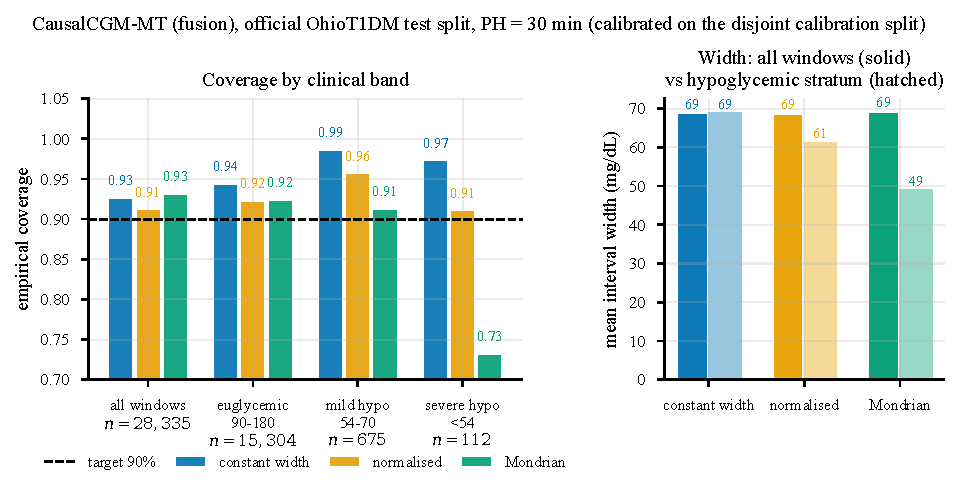
\includegraphics[width=\textwidth]{fig4_conformal_coverage.pdf}
  \caption{Empirical coverage by clinical band and mean interval width for three
  conformal constructions on identical predictions and rows, $\PH = 30$~min,
  $\alpha = \NumAlpha$ (calibrated on the disjoint calibration split, never on
  the validation rows that selected the checkpoint). Mondrian equalises coverage across zones; on this model
  that means \emph{narrowing} the hypoglycemic interval rather than widening it.}
  \label{fig:coverage}
\end{figure*}

A four-zone taxonomy splitting $<54$ out is the obvious response, and at this
sample size it is statistically unavailable rather than merely inconvenient. Two
conditions bind. The first is feasibility: a stratum can certify level $\alpha$
only once it holds $\lceil (1-\alpha)/\alpha \rceil$ calibration points, below
which the required order statistic does not exist and our
\texttt{conformal\_quantile} returns $+\infty$ by construction rather than
falling back to the sample maximum. The second, and the binding one here, is
variance. Conditional on the calibration draw, split-conformal coverage is
$\mathrm{Beta}(n + 1 - \ell,\, \ell)$ with $\ell = \lfloor (n+1)\alpha \rfloor$,
so its standard deviation is of order $\sqrt{\alpha(1-\alpha)/n}$. The $<54$ test cell
holds $\NumSevereN$ windows, so coverage measured in it has a sampling standard
deviation of the same order, near $\NumSevereCovSDPts$ percentage points, before the interval half-width (itself an extreme order
statistic of a small sample) contributes its own dispersion. A dedicated
stratum would therefore certify a conditional guarantee whose realised coverage
moves, from calibration draw to calibration draw, by an amount comparable to the
miscoverage it was introduced to repair. The estimator's variance would dominate
the effect it estimates, which is a worse instrument than the pooled quantile it
replaced, not a better one.

The alternative is to leave the quantile pooled and make the \emph{width}
locally adaptive, which is what the normalised construction does: it scales one
calibration quantile by $\sigma$, the mean absolute glucose change over the last
30 minutes of the input window (\texttt{rate\_of\_change\_difficulty}). Nothing
in $\sigma$ is fitted; it is a fixed function of the history, so it adds no
estimation variance of its own, but it also carries no guarantee that it tracks
difficulty in the severe tail.

The measurements do not separate split and normalised conformal in that cell. Normalised
conformal reaches $\NumNormSevereCov$ coverage below 54~mg/dL, against
$\NumSplitSevereCov$ for split conformal and $\NumMondrianSevereCov$ for
Mondrian, at a mean width of $\NumNormWidth$~mg/dL against $\NumSplitWidth$, and
holds the hypoglycemic band at $\NumNormHypoCov$ against split conformal's
$\NumSplitHypoCov$. Mondrian's narrower hypoglycemic width
($\NumMondrianHypoWidth$~mg/dL, against $\NumNormHypoWidth$ for normalised and
$\NumSplitHypoWidth$ for split conformal) is bought with the
severe-tail undercoverage above. Because the severe cell is small and
autocorrelated, we report the spread of each construction's coverage there
across block-bootstrap resamples of the calibration split (resampling
subject-days, recalibrating, and rescoring the fixed test windows) rather than a
single realisation, and make no recommendation that this spread does not
support.

\paragraph{Which regime one is in.}
We stress that these are properties of \emph{this} model on \emph{this} split.
On a patient-disjoint arm with a weaker model we observe the more commonly
reported pattern instead: severe undercoverage below 70 that stratification
substantially repairs. Which regime one is in should be measured, and we ship
\texttt{scripts/verify\_mondrian\_coverage.py} for that purpose rather than
asserting a figure in prose.

% Appendix E -- the two studies that do not fit the twelve-subject benchmark:
% corpus-scale external validation, and the full personalisation sweep.
\section{Large-Scale Studies: Corpus Validation and Personalisation}
\label{app:largescale}

\subsection{External Validation at Corpus Scale}
\label{sec:metabonet}

% causalcgm-mt-provenance: fingerprint=bc8b1ec3d72b4329 smoke=false generated=2026-10-06T21:08:00
\begin{table*}[t]
\centering
\small
\setlength{\tabcolsep}{4pt}
\caption{MetaboNet benchmark at PH~=~30~min, 5-fold patient-wise cross validation over 1838 subjects from 11 source studies (AZT1D, BrisT1D, CTR3, DCLP3, DCLP5, Flair, IOBP2, Loop, PEDAP, ReplaceBG, T1D-UOM). Whole subjects are held out, so the protocol measures generalisation to an unseen individual; MetaboNet's own \texttt{is\_test} column is a within-subject temporal split and is not used here. OhioT1DM and HUPA-UCM are excluded from the corpus, since both are benchmarks reported elsewhere in this work. Values are means over folds.}
\label{tab:metabonet_comparison}
\resizebox{\ifdim\width>\linewidth\linewidth\else\width\fi}{!}{%
\begin{tabular}{lrrrrrrrrrrrr}
\toprule
Model & RMSE & MAE & MARD (\%) & Lag (min) & A+B (\%) & D+E ($n$) & Parkes A+B (\%) & PR-AUC & Se@5\% & Se@10\% & FAPD@5\% & Onset lead (min) \\
\midrule
cgm\_only & 23.38 & 16.08 & 11.37 & \textbf{22.0} & 98.55 & 2016 & 99.38 & 0.820 & 0.875 & 0.941 & 3.87 & \textbf{22.3} \\
fusion & \textbf{23.08} & \textbf{15.87} & \textbf{11.22} & 22.5 & \textbf{98.58} & \textbf{1970} & \textbf{99.40} & \textbf{0.822} & \textbf{0.875} & \textbf{0.942} & 3.58 & 22.3 \\
\bottomrule
\end{tabular}}
\end{table*}


\begin{figure*}[t]
  \centering
  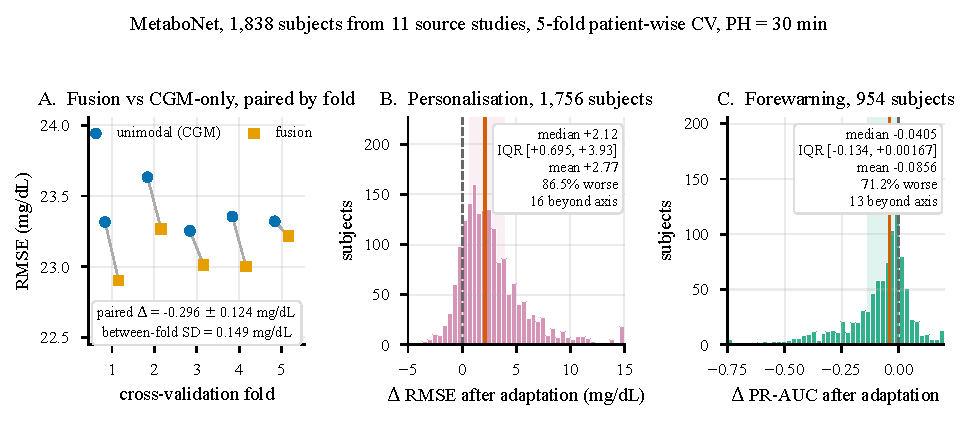
\includegraphics[width=\textwidth]{fig7_metabonet_corpus_scale.pdf}
  \caption{Corpus-scale external validation on MetaboNet,
  $\PH = \NumMetaboHorizon$~min. (A)~Fusion against the CGM-only model, paired
  by fold: both arms are trained on identical splits. (B)~Few-shot LoRA
  adaptation from a $\NumMetaboPersPrefixHours$-hour prefix, per held-out
  subject; positive is worse, the dashed line is no change, the shaded band the
  interquartile range. (C)~The same subjects' forewarning PR-AUC, over the
  $\NumMetaboPersPRAUCSubjects$ whose evaluation region contains hypoglycemia at
  all; negative is worse. Long tails are clipped to the axis with the clipped
  count stated, not dropped.}
  \label{fig:metabonet}
\end{figure*}

This appendix re-measures two OhioT1DM findings on MetaboNet~\citep{wolff2026metabonet},
a consolidated corpus of CGM studies stacked into one table: whether auxiliary fusion improves
on the CGM-only model, and whether few-shot personalisation from a one-day
prefix degrades the population model. $\NumMetaboSources$ source studies
contribute $\NumMetaboSubjects$ subjects. OhioT1DM and HUPA-UCM are excluded as
this paper's own benchmarks; ShanghaiT1DM contributes no window that clears the
gap and observability filters of invariants~I1--I2; and the SIESTA study, added
to the public release after our original analysis, is excluded so that the
corpus matches the one first analysed.

Most of these data were recorded under automated insulin delivery. In
$\NumMetaboCLStudies$ of the $\NumMetaboSources$ contributing studies the
released records come from automated insulin delivery systems, and these studies
supply $\NumMetaboCLSubjPct\%$ of the subjects; $\NumMetaboCLMixedStudies$
more mix automated and non-automated periods or participants, and
$\NumMetaboCLNoStudies$ used none (per-study classes and sources:
\texttt{manuscript/metabonet\_study\_design.json}). Not all of these studies
are trials: the largest source is an observational study of a community-built
system. In such data part of the insulin signal may reflect a controller
responding to glucose rather than an independent input.

\paragraph{The corpus contains this paper's benchmarks, and that is disqualifying.}
The release we analysed includes two of this paper's benchmarks, OhioT1DM and
HUPA-UCM:
all twelve Ohio subjects, including the CGM samples that fall inside the official
\emph{test} spans, every row labelled as training data. Fitting on the
consolidated corpus and reporting on either benchmark is training on the test
set, and the resulting metrics would improve rather than fail visibly.
OhioT1DM and HUPA-UCM are therefore dropped from the corpus by default and the
loader refuses them explicitly. A second hazard is quieter: subject
identifiers collide across source studies, so a bare identifier is not a subject
key and a patient-wise split built on one leaks a person across the fold
boundary. Keys are composite throughout.

\paragraph{Protocol.} Whole subjects are held out under
$\NumMetaboFolds$-fold patient-wise cross validation, so the question asked is
generalisation to an unseen individual. MetaboNet ships an \texttt{is\_test}
column, but it marks a \emph{within}-subject temporal split and answers the
other question; mixing rows from both into one table is the confusion
Section~\ref{sec:setup} refuses for OhioT1DM, and the same rule applies here.
Windowing the whole corpus at stride~1 would produce two orders of magnitude
more tensor data than the machine has memory for, so each subject contributes
at most $\NumMetaboCap$ windows, drawn as
contiguous blocks spread across the record rather than every $k$-th anchor.
Thinning by stride would sever every alarm episode at a sampling gap and empty
the lead-time and false-alarm metrics without emptying the table. That leaves
$\NumMetaboWindows$ windows at a hypoglycemia prevalence of
$\NumMetaboHypoPrev\%$, which is the floor the unimodal arm's
$\NumMetaboCGMPRAUC$ PR-AUC should be read against.

\paragraph{Fusion versus CGM-only.} The submitted version of this analysis
reported that the fusion arm landed on the unimodal baseline. That result was an
artefact: a defect in the per-window presence gate kept insulin and
carbohydrate channels, which carry no observation mask, from ever enabling the
fusion branch, so it opened only on windows carrying a masked wearable stream. With the gate corrected the
branch is active on $\NumMetaboFusionActiveMinPct$--$\NumMetaboFusionActiveMaxPct\%$
of test windows per fold. Fusion then lowers RMSE in all
$\NumMetaboFusionRMSEBetterFolds$ folds: the fold-paired difference is
$\NumMetaboFusionDeltaRMSE \pm \NumMetaboFusionDeltaRMSESD$~mg/dL, about
$\NumMetaboFusionEffectToSpread\times$ the between-fold spread of the CGM-only
arm ($\NumMetaboFoldSDRMSE$~mg/dL). It lowers false alarms per day (fold-paired
difference $\NumMetaboFusionDeltaFAPD \pm \NumMetaboFusionDeltaFAPDSD$; lower in
$\NumMetaboFusionFAPDBetterFolds$ of $\NumMetaboFolds$ folds). Its PR-AUC gain,
$\NumMetaboFusionDeltaPRAUC \pm \NumMetaboFusionDeltaPRAUCSD$, is negligible, and
its effect on Clarke zone D/E counts is not resolved
($\NumMetaboFusionDeltaDE \pm \NumMetaboFusionDeltaDESD$; fewer in
$\NumMetaboFusionDEBetterFolds$ of $\NumMetaboFolds$ folds). This replicates the
direction of the OhioT1DM point-accuracy gain at a smaller magnitude. Because
cross-validation folds share training subjects, the per-fold differences are not
independent replicates, and we report their spread and sign counts rather than a
significance test. In the automated-insulin-delivery studies, part of what the
insulin channels carry may be the controller's own response to falling glucose,
so this gain should be read as what the recorded treatment channels add to CGM,
not as evidence about insulin as an independent physiological input. Lead
time in Table~\ref{tab:metabonet_comparison} is measured to onset, as in
Section~\ref{sec:results}.

\paragraph{The personalisation failure replicates, in the regime we said was
open.} Section~\ref{sec:personalisation} cannot test adaptation to a subject the
population model has never seen, which is the regime few-shot personalisation is
usually claimed for. Patient-wise cross validation is that protocol. It scores
$\NumMetaboPersSubjects$ of the $\NumMetaboSubjects$ corpus subjects: the paired
design needs a full adaptation prefix, one embargo, and at least 50 evaluation
windows after it, all from one subject's kept windows, and $\NumMetaboPersSkipped$ records are too
short to supply all three. They are skipped rather than scored on a truncated
prefix, an exclusion that turns on record length rather than on the subject's
glycemia and is applied before any adaptation runs. Each of the
$\NumMetaboPersSubjects$ is adapted from a
$\NumMetaboPersPrefixHours$-hour prefix of its own record (a median of
$\NumMetaboPersAdaptWindows$ windows) with LoRA at rank~$\NumMetaboPersRank$,
$\NumMetaboPersTrainable$ trainable parameters, and scored on its own
post-embargo region. The held-out test rows themselves cannot be used, because
under this protocol they contain the prefix the adaptation was fitted on. Adaptation costs $\NumMetaboPersDeltaRMSE$~mg/dL of RMSE on average; the
median subject loses $\NumMetaboPersMedianDeltaRMSE$~mg/dL, the interquartile
range $[\NumMetaboPersDeltaRMSEQOne, \NumMetaboPersDeltaRMSEQThree]$ lies
entirely above zero, and $\NumMetaboPersWorsePct\%$ of subjects are worse after
adapting than before. Only $\NumMetaboPersImproved$ of
$\NumMetaboPersSubjects$ improve (Figure~\ref{fig:metabonet}B). The forewarning
task degrades too, on a smaller base: PR-AUC is undefined for a subject
whose evaluation region contains no hypoglycemia at all, so the mean change of
$\NumMetaboPersDeltaPRAUC$ is over the $\NumMetaboPersPRAUCSubjects$ subjects
where both sides are defined, $\NumMetaboPersPRAUCWorsePct\%$ of whom are worse
(Figure~\ref{fig:metabonet}C).
The sign matches OhioT1DM's $\NumPersLoRAFourRMSEDelta$~mg/dL, at
$\NumMetaboPersOhioPct\%$ of its magnitude. Here the adaptation data are
genuinely new to the population model, which the OhioT1DM design could not
ensure. The adaptation recipe is unchanged, however: a fixed step budget with no
held-out early stopping. This result therefore shows that this recipe degrades
unseen subjects too; it does not separate scarce data from over-adaptation as
the cause.

\paragraph{What this appendix does not establish.} One seed, one horizon
($\PH = \NumMetaboHorizon$~min), one adapter, one prefix length. The per-subject
window cap makes a long record contribute no more than a short one. The tabular
and classical baselines of Section~\ref{sec:baselines} were not re-fitted at this
scale; the only external reference is persistence at
$\NumMetaboPersistRMSE$~mg/dL.

\subsection{Few-Shot Personalisation: A Negative Result}
\label{sec:personalisation}

The OhioT1DM protocol is temporal and \emph{within} patient, which makes
per-subject adaptation the natural question to ask of it. We adapt the
population model to each of $\NumPersSubjects$ subjects from a
$\NumPersPrefixHours$-hour prefix of that subject's own training file, separated
from every evaluation window by the embargo of invariant~I5, and compare before
and after on \emph{identical} windows. Those windows are the official test file
alone. The prefix--embargo geometry separates the \emph{adaptation} data from the
evaluation data, but it says nothing about the \emph{population} model, which was
fitted on the training file the prefix is drawn from; scoring on the remainder of
that file as well would leave most of the evaluation region in-sample for the
zero-shot arm the deltas are measured against. Restricting to the released
testing windows costs roughly half the hypoglycemic events and is the only set
disjoint from both the fit and the model-selection split. Six arms are tested: no adaptation and five adapted modes,
BatchNorm statistic recalibration~\citep{schneider2020improving}, LoRA~\citep{hu2022lora} at ranks 4 and 8 with
an L2-SP anchor~\citep{xuhong2018explicit}, head-only fine-tuning, and full
fine-tuning. Because five adapted modes are tested at each prefix length, $p$-values are
Holm--Bonferroni adjusted~\citep{holm1979simple} within that family.

At the default budget of $\NumPersDefaultSteps$ gradient steps and the
$\NumPersPrefixHours$-hour prefix (Table~\ref{tab:personalization}), every
adapted mode makes the model worse on RMSE and PR-AUC, and the effects are not
marginal. At $\PH = 30$~min, BatchNorm adaptation costs $\NumPersBNAdaptRMSEDelta$~mg/dL RMSE
($p_{\text{Holm}} = \NumPersBNAdaptRMSEP$) and
$\NumPersBNAdaptPRAUCDelta$ PR-AUC; LoRA at rank~4 costs
$\NumPersLoRAFourRMSEDelta$~mg/dL and $\NumPersLoRAFourPRAUCDelta$ PR-AUC; full
fine-tuning costs $\NumPersFullRMSEDelta$~mg/dL and
$\NumPersFullPRAUCDelta$ PR-AUC. RMSE improved for
$\NumPersLoRAFourRMSEImproved$ of $\NumPersSubjects$ subjects under LoRA.
False-alarm rates are not reported for the adapted models: alarm thresholds are
fitted on calibration data, and this protocol has none for a per-subject model.

Two diagnostics describe the damage. First, it grows with the adaptation
budget: LoRA at rank~4 changes RMSE by $\NumPersLoRAStepsTenDelta$~mg/dL after
ten gradient steps and $\NumPersLoRAStepsTwoHundredDelta$ after two hundred.
That is the signature of over-adaptation to the prefix, and no mode here uses
held-out early stopping to prevent it. Second, BatchNorm adaptation, which
recomputes running statistics on the prefix and updates no weights, also
degrades the model: by $\NumPersBNPrefixSixDelta$~mg/dL from a six-hour prefix
(over $\NumPersPrefixSixN$ subjects; the other prefix lengths use all
$\NumPersPrefixTwentyFourN$),
$\NumPersBNPrefixTwentyFourDelta$ from twenty-four hours and
$\NumPersBNPrefixFortyEightDelta$ from forty-eight. Replacing population
activation statistics with one subject's is therefore harmful in itself, and the
cost stops shrinking after a day of data, which a pure estimation-noise account
would not predict. Head-only fine-tuning, by contrast, keeps improving with
prefix length ($\NumPersHeadPrefixSixDelta \to
\NumPersHeadPrefixFortyEightDelta$~mg/dL from six to forty-eight hours, the
six-hour value over $\NumPersPrefixSixN$ subjects and the rest over
$\NumPersPrefixTwentyFourN$) without reaching zero.

These diagnostics do not isolate a single cause. Scarce adaptation data,
over-adaptation under a fixed step budget, and the loss of population
statistics are all consistent with them, and the design cannot separate them:
on OhioT1DM the prefix lies inside the population model's own training split, so
adaptation adds no new information.

\begin{table*}[t]
\centering
\small
\setlength{\tabcolsep}{4pt}
\caption{Few-shot personalisation on OhioT1DM, PH = 30 min, 24 h adaptation prefix, 12 subjects. $\Delta$ is the paired per-subject change from the zero-shot population model on identical evaluation windows; $p$ is a paired $t$-test with Holm--Bonferroni adjustment across modes. The zero-shot baseline reads 18.84~mg/dL here against 18.97~mg/dL in Table~\ref{tab:sota_ph30}: the same checkpoint on the same 28,335 windows, aggregated differently. This table averages the 12 per-subject RMSEs, which is the quantity the paired tests are computed on; Table~\ref{tab:sota_ph30} pools the residuals across all windows. Weighting these rows by their window counts recovers the pooled RMSE exactly (18.968 against 18.97). PR-AUC does not decompose this way: it is a rank statistic over the pooled residuals, so the per-subject mean (0.790, sd 0.145, range 0.566--0.954 across the 12 subjects) is a different quantity from the pooled 0.870 and is not recoverable from it by reweighting. The paired tests are computed on the per-subject values reported here.}
\label{tab:personalization}
\resizebox{\ifdim\width>\linewidth\linewidth\else\width\fi}{!}{%
\begin{tabular}{lrrrrrrrrr}
\toprule
Adaptation & RMSE & $\Delta$ RMSE & $p_{\mathrm{Holm}}$ & PR-AUC & $\Delta$ PR-AUC & $p_{\mathrm{Holm}}$ & FAPD@5\% & $\Delta$ FAPD@5\% & $p_{\mathrm{Holm}}$ \\
\midrule
none & \textbf{18.844} & \textbf{+0.000} & -- & \textbf{0.790} & \textbf{+0.000} & -- & -- & -- & -- \\
bn\_adapt & 19.887 & +1.043 & 0.008 & 0.733 & -0.057 & 0.063 & -- & -- & -- \\
lora (r=4) & 21.678 & +2.834 & 0.000 & 0.686 & -0.105 & 0.063 & -- & -- & -- \\
lora (r=8) & 21.366 & +2.522 & 0.000 & 0.678 & -0.112 & 0.036 & -- & -- & -- \\
head\_only & 19.545 & +0.701 & 0.022 & 0.734 & -0.056 & 0.033 & -- & -- & -- \\
full & 22.826 & +3.982 & 0.000 & 0.697 & -0.094 & 0.006 & -- & -- & -- \\
\bottomrule
\end{tabular}}
\end{table*}

\begin{table*}[t]
\centering
\small
\setlength{\tabcolsep}{4pt}
\caption{Adaptation budget: mean paired $\Delta$RMSE (mg/dL) as a function of the number of gradient steps, at a 24 h prefix and PH = 30 min. For LoRA at both ranks the damage grows with every increase in the budget; head-only fine-tuning is not monotone.}
\label{tab:step_budget}
\resizebox{\ifdim\width>\linewidth\linewidth\else\width\fi}{!}{%
\begin{tabular}{lrrrrr}
\toprule
Adaptation & 10 steps & 25 steps & 50 steps & 100 steps & 200 steps \\
\midrule
lora (r=4) & -0.018 & +0.378 & +1.078 & +1.873 & +2.834 \\
lora (r=8) & -0.055 & +0.240 & +0.886 & +1.726 & +2.522 \\
head\_only & \textbf{-0.221} & \textbf{-0.287} & \textbf{-0.111} & \textbf{+0.225} & \textbf{+0.701} \\
\bottomrule
\end{tabular}}
\end{table*}


The natural explanation is within-subject drift. A short prefix would then be an
unrepresentative sample of the subject's \emph{own} later distribution: glucose
dynamics move within a person across weeks, so the opening day of a record is a
biased estimate of the month that follows, and adapting to it pulls the model
away from the evaluation period rather than toward it. On this cohort the
opening prefix ends a median of $\NumPosOpeningGapDays$~days before the first
scored window, which is ample room for such a decoupling.

\paragraph{The drift explanation is testable, and it fails.} If staleness were
the mechanism, a prefix drawn from the evaluation window's own temporal
neighbourhood should not fail the same way. We therefore add a
\emph{prefix-position} control: the same $\NumPersPrefixHours$ hours, the same
subjects, the same evaluation windows, the same adapter and the same step
budget, but taken from the \emph{end} of the training file so that the prefix
closes exactly one embargo ($\NumPosRecentGapMin$~minutes) before the first
scored window. Only the distance between the adaptation data and the scored data
changes. The sweep records where each prefix lies relative to the population
model's fit and model-selection rows. All $\NumPosOpeningAdaptWindowsTotal$ adaptation
windows of the opening prefix, summed over subjects, lie in the fit rows. None of
the $\NumPosRecentAdaptWindowsTotal$ recent-prefix windows lies in the fit rows
($\NumPosRecentAdaptInFit$) or in the model-selection rows
($\NumPosRecentAdaptInVal$). The contrast therefore changes recency and also
whether the adaptation windows were seen in training; it does not separate the two.

\begin{table*}[t]
\centering
\small
\setlength{\tabcolsep}{4pt}
\caption{Adaptation prefix position at a 24 h prefix, PH = 30 min. Both arms use the same subjects, evaluation windows, adapter, step budget and prefix length; they differ only in how far the prefix sits from the windows being scored. The opening prefix ends a median of 44~days before the first scored window; the recent prefix ends 185~min before it, which is the embargo itself. No column of paired differences is significant, and no arm becomes an improvement over zero-shot under either position. Negative $\Delta$RMSE and positive $\Delta$PR-AUC are better.}
\label{tab:prefix_position}
\resizebox{\ifdim\width>\linewidth\linewidth\else\width\fi}{!}{%
\begin{tabular}{lrrrrrrrr}
\toprule
Adaptation & $\Delta$RMSE open & $\Delta$RMSE recent & rec$-$open & $p_{\mathrm{Holm}}$ & $\Delta$PR-AUC open & $\Delta$PR-AUC recent & rec$-$open & $p_{\mathrm{Holm}}$ \\
\midrule
none & +0.000 & +0.000 & +0.000 & -- & +0.000 & +0.000 & +0.000 & -- \\
bn\_adapt & +1.043 & +1.521 & +0.478 & 0.977 & -0.057 & -0.046 & +0.011 & 1.000 \\
lora (r=4) & +2.834 & +3.754 & +0.920 & 0.888 & -0.105 & -0.154 & -0.049 & 1.000 \\
lora (r=8) & +2.522 & +3.313 & +0.791 & 0.699 & -0.112 & -0.154 & -0.042 & 1.000 \\
head\_only & +0.701 & +1.566 & +0.865 & 0.888 & -0.056 & -0.041 & +0.015 & 1.000 \\
full & +3.982 & +4.209 & +0.227 & 0.977 & -0.094 & -0.196 & -0.102 & 0.412 \\
\bottomrule
\end{tabular}}
\end{table*}


Recency does not rescue adaptation. At the default step budget, every adapted
mode still raises RMSE from a recent prefix, and significantly so: BatchNorm adaptation costs
$\NumPosRecentBNAdaptRMSEDelta$~mg/dL ($p_{\text{Holm}} =
\NumPosRecentBNAdaptRMSEP$), LoRA at rank~4 $\NumPosRecentLoRAFourRMSEDelta$
($p_{\text{Holm}} = \NumPosRecentLoRAFourRMSEP$) and full fine-tuning
$\NumPosRecentFullRMSEDelta$ ($p_{\text{Holm}} = \NumPosRecentFullRMSEP$). The
paired recent-minus-opening differences are null throughout, and no mode does
better from the recent prefix: every difference is positive, the smallest being
$\NumPosBestDiffRMSE$~mg/dL (raw $p = \NumPosBestDiffP$). For LoRA at rank~4 the
95\% confidence interval of the difference,
$[\NumPosDiffLoRAFourRMSECILow, \NumPosDiffLoRAFourRMSECIHigh]$, straddles zero;
the smallest Holm-adjusted $p$ across all modes is $\NumPosMinDiffPHolm$. Head-only
fine-tuning is nominally \emph{worse} from the recent prefix
($\NumPosDiffHeadOnlyRMSE$~mg/dL), and full fine-tuning is worse on forewarning
($\NumPosDiffFullPRAUC$ PR-AUC). Moving the adaptation data
$\NumPosOpeningGapDays$~days closer to the windows being scored changes
essentially nothing.

The prefix-position control therefore gives no support to drift as the
explanation: a recent prefix degrades the model as much as an opening one, within
the precision twelve subjects allow.

The reading we can support is narrow. With this recipe (a prefix of at most 48
hours, no held-out early stopping), at the default step budget and the
$\NumPersPrefixHours$-hour prefix every adapted mode degrades the population
model on OhioT1DM, and shipping the population model unchanged is the better of
those configurations. Very short head-only budgets are the exception on RMSE
(Table~\ref{tab:step_budget}): $\NumPersHeadOnlyStepsTenDelta$~mg/dL after ten steps,
$\NumPersHeadOnlyStepsTwentyFiveDelta$ after twenty-five and
$\NumPersHeadOnlyStepsFiftyDelta$ after fifty, with $\NumPersHeadStepsTenImproved$ of
$\NumPersSubjects$ subjects improving at ten steps. The ten-step interval,
$[\NumPersHeadStepsTenCILow, \NumPersHeadStepsTenCIHigh]$ with $p =
\NumPersHeadStepsTenP$, is unadjusted: the step-budget cells carry no multiplicity
correction, so we do not call it significant. Mean PR-AUC does not improve at any
budget for any adapter in that table. Whether longer prefixes, genuinely new adaptation
data or held-out early stopping change that remains open. A held-out-subject
protocol, the regime few-shot personalisation is usually claimed for, is tested
in Appendix~\ref{sec:metabonet}: on $\NumMetaboPersSubjects$ unseen subjects the
same adapter and prefix length cost $\NumMetaboPersDeltaRMSE$~mg/dL.


\end{document}
